% Options for packages loaded elsewhere
\PassOptionsToPackage{unicode}{hyperref}
\PassOptionsToPackage{hyphens}{url}
%
\documentclass[
]{krantz}
\usepackage{lmodern}
\usepackage{amssymb,amsmath}
\usepackage{ifxetex,ifluatex}
\ifnum 0\ifxetex 1\fi\ifluatex 1\fi=0 % if pdftex
  \usepackage[T1]{fontenc}
  \usepackage[utf8]{inputenc}
  \usepackage{textcomp} % provide euro and other symbols
\else % if luatex or xetex
  \usepackage{unicode-math}
  \defaultfontfeatures{Scale=MatchLowercase}
  \defaultfontfeatures[\rmfamily]{Ligatures=TeX,Scale=1}
\fi
% Use upquote if available, for straight quotes in verbatim environments
\IfFileExists{upquote.sty}{\usepackage{upquote}}{}
\IfFileExists{microtype.sty}{% use microtype if available
  \usepackage[]{microtype}
  \UseMicrotypeSet[protrusion]{basicmath} % disable protrusion for tt fonts
}{}
\makeatletter
\@ifundefined{KOMAClassName}{% if non-KOMA class
  \IfFileExists{parskip.sty}{%
    \usepackage{parskip}
  }{% else
    \setlength{\parindent}{0pt}
    \setlength{\parskip}{6pt plus 2pt minus 1pt}}
}{% if KOMA class
  \KOMAoptions{parskip=half}}
\makeatother
\usepackage{xcolor}
\IfFileExists{xurl.sty}{\usepackage{xurl}}{} % add URL line breaks if available
\IfFileExists{bookmark.sty}{\usepackage{bookmark}}{\usepackage{hyperref}}
\hypersetup{
  pdftitle={Apuntes de Economía y Administración de Empresas},
  pdfauthor={Saúl Torres-Ortega},
  hidelinks,
  pdfcreator={LaTeX via pandoc}}
\urlstyle{same} % disable monospaced font for URLs
\usepackage{longtable,booktabs}
% Correct order of tables after \paragraph or \subparagraph
\usepackage{etoolbox}
\makeatletter
\patchcmd\longtable{\par}{\if@noskipsec\mbox{}\fi\par}{}{}
\makeatother
% Allow footnotes in longtable head/foot
\IfFileExists{footnotehyper.sty}{\usepackage{footnotehyper}}{\usepackage{footnote}}
\makesavenoteenv{longtable}
\usepackage{graphicx,grffile}
\makeatletter
\def\maxwidth{\ifdim\Gin@nat@width>\linewidth\linewidth\else\Gin@nat@width\fi}
\def\maxheight{\ifdim\Gin@nat@height>\textheight\textheight\else\Gin@nat@height\fi}
\makeatother
% Scale images if necessary, so that they will not overflow the page
% margins by default, and it is still possible to overwrite the defaults
% using explicit options in \includegraphics[width, height, ...]{}
\setkeys{Gin}{width=\maxwidth,height=\maxheight,keepaspectratio}
% Set default figure placement to htbp
\makeatletter
\def\fps@figure{htbp}
\makeatother
\setlength{\emergencystretch}{3em} % prevent overfull lines
\providecommand{\tightlist}{%
  \setlength{\itemsep}{0pt}\setlength{\parskip}{0pt}}
\setcounter{secnumdepth}{5}
\usepackage{booktabs}

\ifxetex
  \usepackage{polyglossia}
  \setmainlanguage{spanish}
  % Tabla en lugar de cuadro
  \gappto\captionsspanish{\renewcommand{\tablename}{Tabla}  
          \renewcommand{\listtablename}{Índice de tablas}}
\else
  \usepackage[spanish,es-tabla]{babel}
\fi
\usepackage[]{natbib}
\bibliographystyle{apalike}

\title{Apuntes de Economía y Administración de Empresas}
\author{Saúl Torres-Ortega}
\date{2020-08-20}

\begin{document}
\maketitle

{
\setcounter{tocdepth}{2}
\tableofcontents
}
\hypertarget{portada}{%
\chapter*{Portada}\label{portada}}


Bienvenida/os.

\hypertarget{introducciuxf3n}{%
\chapter*{Introducción}\label{introducciuxf3n}}


Son ya unos cuantos años los que llevo impartiendo docencia de economía y administración de empresas. Desde mis primeras clases, allá por el año 2010, he ido creando y mejorando los distintos materiales que he ido utilizando.

Sin embargo, con el paso del tiempo, he ido notando que más allá de unas buenas transparencias y una buena colección de ejercicios, problemas y prácticas, lo que sin duda puede ser una diferencia es tener unos buenos apuntes que vayan más allá de las meras enumeraciones y definiciones en las que se suelen convertir las transparencias docentes, y marquen un determinado discurso y permitan profundizar un poco en los conceptos explicados.

Lo ideal sin duda alguna era poder recomendar a mis alumnos un libro de referencia con el que poder seguir la asignatura. Afortunadamente manuales de introducción a la economía y a la administración de empresas hay muchos. Sin embargo, recomendar un libro de 400-500 páginas para un curso introductorio en el que ese contenido se puede ver en 5-8 semanas de clase es, desde mi punto de vista, un pequeño despropósito.

Con estos todos pensamientos en mi cabeza, y toda vez que parecía tener clara la necesidad de tener que fabricarme algo a mi gusto y totalmente adaptado, me faltaba la forma de articularlo. Después de unos años trasteando con \texttt{R}, lenguaje de programación que poco a poco he ido aprendiendo y con el que he ido descubriendo como hacer cada día más cosas, llegué hasta el paquete \href{https://bookdown.org/}{Bookdown}. Más o menos, y de una forma muy breve, es un paquete que permite crear una estructura de libro utilizando el lenguaje \emph{Markdown}. ¿Ventajas que le veo? Tener actualizado y online (y por tanto disponible para mis alumnos) este compendio de apuntes sin tener que preocuparme demasiado de formatos ni estructuras.

Espero poder decir dentro de un par de años que este experimento ha fraguado correctamente, y que quienes lo estáis leyendo, podéis tener aquí algo así como un que os sirva para el estudio y nos permita dedicar el tiempo de clase a interiorizar los conceptos más que a aprender sobre ellos.

Sea como fuera, aquí está este documento.

\hypertarget{por-quuxe9-leer-este-libro}{%
\section*{¿Por qué leer este libro?}\label{por-quuxe9-leer-este-libro}}


Se me ocurre una razón fundamental: soy tu profesor y te lo he recomendado. Si es así, bueno, supongo que lo mejor que puedes hacer es hacerme caso y usar este documento como base para tu estudio y seguir la asignatura.

Puede sin embargo que por otra razón del destino hayas acabado aquí. En ese caso, supongo que habrá algún aspecto del libro que pueda serte de ayuda. Sinceramente, espero que así sea.

\hypertarget{estructura-del-libro}{%
\section*{Estructura del libro}\label{estructura-del-libro}}


El documento está dividido en tres grandes bloques, los mismos en los que suele estar dividida la asignatura. Un primer bloque que aborda el entorno económico de la empresa, donde se verá el funcionamiento básico de la economía, tanto desde la vertiente de la microeconomía (oferta, demanda, mercados), como de la macroeconomía (mercados agregados y políticas), y los entornos genérico y específico. El segundo bloque se introduce en la administración de la empresa: planificación, organización y gestión de los recursos humanos. Además, se dedicará atención a la contabilidad, financiación e inversión en la empresa. Por último, el tercer y último bloque se centra en toda la dirección de la producción y operaciones de la empresa.

Casi todos los contenidos tienen un carácter básico e introductorio, con una visión bastante aplicada a la ingeniería, y están enfocados principalmente a una asignatura general de economía y administración de empresas de nivel de grado. Sin embargo, en algunas secciones aparecerán contenidos con un mayor nivel de detalle, más avanzados y con un mayor grado de aplicación, que están pensados para una asignatura de nivel de máster.

\hypertarget{lecturas-recomendadas}{%
\section*{Lecturas recomendadas}\label{lecturas-recomendadas}}


Lo que tienes entre manos (o en la pantalla de tu ordenador, en todo caso delante de los ojos) es una versión muy previa de lo que algún día serán unos buenos apuntes. De momento es un compendio de las secciones más relevantes que he encontrado en alguno de los manuales de economía y empresa que han pasado por mis manos y más me han gustado y que paso a enumerar. Para ampliar cualquiera de los contenidos, no tienes más que recurrir a ellos, pues cualquiera de estos libros contiene mucho mayor detalle en los distintos temas abordados, y que de nuevo al estar estos apuntes enfocados a una asignatura de carácter introductorio, son vistos sin profundidad aquí.

\begin{itemize}
\tightlist
\item
  Juan Manuel Blanco. ``Economía: teoría y práctica''. McGraw Hill España. 5ª edición.
\item
  Gregor N. Mankiw. ``Principios de economía''. Cengage Learning España. 7ª edición.
\item
  Michael Parkin. ``Economía''. Pearson Education. 12ª edición.
\item
  Bueno Campos. ``Principios de administración de empresas''.
\end{itemize}

\hypertarget{agradecimientos}{%
\section*{Agradecimientos}\label{agradecimientos}}


Es de rigor aquí también agradecer a los alumnos que han formado parte de este proceso, porque gracias a los comentarios e interés de algunos de ellos, algunos apartados han ganado en contenidos, calidad y ejemplos.

Voy a permitir el destacar algunos de ellos, que sin duda han colaborado y ayudado más a la elaboración del documento:

\begin{itemize}
\tightlist
\item
  David Fernández Díaz (Curso 2018/2019, Grado en Ingeniería de los Recursos Energéticos)
\end{itemize}

Si has llegado leyendo hasta aquí y detectas en el documento algún error, así como tienes cualquier sugerencia o cambio que crees puede mejorar estos apuntes, no dudes en ponerte en contacto conmigo porque sin duda agradeceré tu interés.

\mainmatter

\hypertarget{part-el-entorno-econuxf3mico-de-la-empresa}{%
\part{El Entorno Económico de la Empresa}\label{part-el-entorno-econuxf3mico-de-la-empresa}}

\hypertarget{quuxe9-es-la-economuxeda}{%
\chapter{¿Qué es la economía?}\label{quuxe9-es-la-economuxeda}}

Según Mick Jagger (el que por cierto posee un título en economía de la London School of Economics) y los Rolling Stones, \href{https://www.youtube.com/watch?v=oqMl5CRoFdk}{``You Can't Always Get What You Want''}, o lo que es lo mismo, ``no puedes siempre conseguir lo que quieres''.

¿Por qué no podemos conseguirlo? Porque todos nosotros (los que a partir de ahora nos llamaremos sujetos económicos y que posteriormente definiremos en profundidad) tenemos por lo general necesidades ilimitadas. Si queremos satisfacer estas necesidades, requeriremos de recursos, que al contrario de lo que sucede con nuestras necesidades, no son ilimitados sino generalmente escasos.

La economía se puede definir como la ciencia que dedica sus esfuerzos al estudio de la forma en que los individuos eligen en condiciones de escasez y de las consecuencias de esas elecciones para la sociedad. En la antigua Grecia, economía hacía referencia a ``administrar el patrimonio'', por eso se define como ``la ciencia de la elección'': administrar es elegir entre distintas opciones \citep{sande2015}.

La economía es la ciencia que estudia el modo en el que una sociedad gestiona sus recursos {[}\citet{mankiw2017}. Uno de los objetivos de la economía es buscar cómo deben asignarse los recursos disponibles para obtener la máxima utilidad de los mismos (o dicho de otra manera, el máximo beneficio). Para ello, a veces la economía recurre a modelos que ayudan a comprender y predecir la realidad. Algunos de ellos son el flujo circular de la renta o la curva frontera de posibilidades de producción.

La \textbf{microeconomia} es una rama de la economía la cual estudia el comportamiento de los agentes individuales (hogares, empresas, sector público) y el funcionamiento de los mercados para asignar los recursos escasos a los distintos usos alternativos.
También estudia como se forman los precios mediante la interacción de los hogares y de las empresas en los distintos mercados.

La \textbf{macroeconomia} es otra rama de la economía que se encarga del estudio de los fenómenos que afectan al conjunto de los grandes agregados económicos (Renta Nacional, PIB\ldots), que nos permiten obtener una visión global de la economía de un país.
Su objetivo principal es comprender y mejorar los resultados de la economía en su entorno mas global.

\hypertarget{los-agentes-econuxf3micos}{%
\section{Los agentes económicos}\label{los-agentes-econuxf3micos}}

Los protagonistas de las actividades económicas somos todos los ciudadanos, también llamados agentes económicos en el entorno de la vida económica. Dependiendo del papel que se juega en la actividad dentro de nuestro sistema, se agrupa en una de estas tres categorías:

\begin{itemize}
\tightlist
\item
  Economía doméstica: Su función es el consumo y el objetivo la máxima satisfacción con unas limitaciones de renta y preferencias.
\item
  Empresas: Se basan en la producción y en el máximo beneficio con limitaciones de presupuesto financiero y tecnología.
\item
  Sector público: Su función es la regulación suministro de bienes públicos y el objetivo es el máximo bienestar económico y colectivo con las limitaciones de los ingresos públicos.
\end{itemize}

\hypertarget{la-escasez-y-el-problema-de-tener-que-decidir}{%
\section{La escasez y el problema de tener que decidir}\label{la-escasez-y-el-problema-de-tener-que-decidir}}

Como hemos dicho anteriormente, los sujetos económicos nos enfrentamos en nuestro día a día a la escasez. La escasez no entendida como un problema tecnológico, sino de disparidad
entre nuestros deseos y los medios de los que disponemos para satisfacerlos.
Por lo tanto, igualmente nos encontramos día a día frente a decisiones que se nos plantean para decidir qué necesidades satisfacemos primero y a cuales debemos renunciar. A la hora de tomar estas decisiones, los sujetos económicos nos basamos en varios principios básicos, presentes en todas y cada una de nuestras decisiones.

\begin{itemize}
\tightlist
\item
  Principio de escasez
\item
  Principio Coste-Beneficio
\item
  Principio de los incentivos
\item
  Principio de eficiencia y equidad
\end{itemize}

\hypertarget{los-costes-econuxf3micos-en-la-toma-de-decisiones}{%
\section{Los costes económicos en la toma de decisiones}\label{los-costes-econuxf3micos-en-la-toma-de-decisiones}}

La economía nos enseña que ``no hay nada gratis''. Dicho de otra forma, todas nuestras decisiones tienen un coste asociado, que es lo que denominamos coste de oportunidad.

\begin{quote}
\textbf{Coste de oportunidad}: es el coste asociado a aquello a lo que se renuncia cuando se toma una decisión. Más concretamente, el coste de oportunidad de un bien o servicio es la cantidad de otros bienes o servicios a la que se debe renunciar para obtenerlo.
\end{quote}

Pongamos un ejemplo. Supongamos que es media mañana y es la hora de nuestra pausa para el almuerzo. Después de haber desayunado a primera hora del día, a esa hora puede ser bastante normal que tengamos tanto hambre como algo de sed. Sin embargo, hemos salido apresurados de casa por la mañana y hemos dejado olvidado nuestro monedero. Tan sólo tenemos 1 euro.
En el bar nos ofrecen bebida y comida, pero el refresco que deseamos cuesta 1 euro y el pincho de tortilla que nos gusta tiene un precio de 1 euro también. Debemos elegir, y debemos renunciar. Si elegimos saciar nuestra sed, y pedimos el refresco, estamos sacrificando el pincho de tortilla. Mantenernos con hambre es por tanto nuestro coste de oportunidad de elegir el refresco. El coste de oportunidad de elegir comer un pincho de tortilla es mantenernos con sed.

Además de este concepto de coste de oportunidad, en nuestras tomas de decisiones aparecen otros costes que también nos influyen desde el punto de vista económico.

\begin{quote}
\textbf{Coste irrecuperable}: es un coste que en cualquiera de las opciones de decisión que nos planteemos, está presente. Al ser un coste que vamos a tener que asumir siempre, independientemente de nuestra decisión, no debería influir en la toma de decisión.
\end{quote}

Sigamos con nuestro ejemplo y supongamos ahora que además de lo anterior, para llegar al bar debemos cruzar una gran avenida, y tenemos la mala suerte de que en este momento está lloviendo a mares. Volviendo a la situación anterior, tanto si elegimos comernos el pincho de tortilla como bebernos el refresco, tendremos un coste adicional, que es estar mojados por la lluvia. Este es un coste irrecuperable.

\begin{quote}
\textbf{Coste de transacción}: es un coste en el que necesariamente incurrimos al realizar un intercambio económico, o más precisamente, una transacción en un mercado.
\end{quote}

La existencia de estos costes de transacción fue desarrollada por primera vez por el economista Ronald Coase en su artículo ``The Nature of the Firm'' \citep{coase1937}. Coase explica que ``cuando se desea operar una transacción en un mercado, es necesario investigar a los contratistas, proporcionarles ciertas informaciones necesarias y establecer las condiciones del contrato, llevar a cabo las negociaciones que instauren un verdadero mercado, establecer una estructura de control de las respectivas prestaciones de obligaciones de las partes, etc.''. Sin embargo, es a John Kenneth Arrow a quien se debe el uso del término ``coste de transacción'' \citep{arrow1969}.

Los costes de transacción los podemos agrupar en tres grandes categorías:

\begin{itemize}
\tightlist
\item
  Costes de investigación e información, que son los costes en los que incurrimos cuando queremos saber si el producto que queremos intercambiar está disponible en el mercado, quién tiene el menor precio, etc. Incluyen la recopilación de la información, la comparación de las alternativas, el análisis de su relación calidad/precio, etc.
\item
  Costes de negociación y de decisión, que son los costes necesarios para llegar a un acuerdo con la otra parte de la negociación (tiempo, redacción de documentos).
\item
  Costes de vigilancia y de ejecución, que son los costes necesarios para asegurar que ambas parten cumplen con lo pactado según los términos acordados, así como los costes de tomar acciones si no se cumple con lo previsto.
\end{itemize}

Imagina que has ido de viaje a la vecina Portugal (Oporto por poner un lugar algo más concreto) por vacaciones y deseas traer un buen regalo a la familia: un juego de toallas. Recorrerte durante toda una tarde la zona más turística de Oporto buscando las mejores ofertas, así como los diseños más adecuados y las toallas de mejor calidad supone un coste de investigación e información. Una vez que has decidido el local con el mejor género y mejores precios, llegar a un acuerdo con el propietario por el juego de 6 toallas que quieres adquirir, supone un coste de negociación. El arte del regateo. Por último, comprobar que el género adquirido es de algodón puro y de buena calidad (con envío de muestra a un laboratorio independiente para su análisis si nos ponemos exquisitos) sería un coste de vigilancia y ejecución. Todos ellos, serían ejemplos de costes de transacción.

\hypertarget{oferta-y-demanda}{%
\chapter{Oferta y demanda}\label{oferta-y-demanda}}

La oferta y la demanda son dos conceptos recurrentes que aparecen cuando hablamos de economía. Son las dos fuerzas o palancas que hacen que las economías de mercado funcionen. La oferta y la demanda determinan la cantidad que se produce de cada bien y el precio al que debe venderse. Y esto lo hacen al interactuar en los mercados. El mercado de un producto está formado por todos los vendedores y compradores de un producto, y por lo tanto, por su oferta y su demanda.

\hypertarget{la-demanda}{%
\section{La demanda}\label{la-demanda}}

La demanda es la cantidad que los consumidores (compradores) desean y pueden comprar en funcion del precio.

\begin{quote}
\textbf{LEY DE LA DEMANDA}:
Manteniéndose todo lo demas constante (\emph{ceteris paribus}), cuando aumenta el precio de un bien, la demanda baja.
\end{quote}

La demanda de mercado de un determinado bien es la suma de todas las demandas individuales que lo integran.

La razón por la que cuando el precio del bien aumenta la cantidad demandada por todos los consumidores disminuye es doble. Por un lado, cuando aumenta el precio de un bien algunos consumidores que previamente lo adquirían dejarán de hacerlo o lo comprarán en menor cuantía y buscarán otros bienes que lo sustituirán. Esto se conoce como efecto sustitución, en el sentido de que el bien o servicio que se encarece relativamente tiende a ser sustituido por otros que ahora resultan más baratos.

Por otro lado, los consumidores cuando un bien se encarece demandarán menos unidades del mismo porque la elevación del precio ha reducido la capacidad adquisitiva de la renta, y esto hará que se pueda comprar menos de todos los bienes y, en particular, del que estamos considerando. Este hecho se conoce como el efecto renta, e indica que un incremento en los precios de un bien, disminuye la capacidad adquisitiva de los consumidores para un nivel de renta dado. Ante esta circunstancia los consumidores se verán motivados a reducir la compra de todos los bienes o servicios.

\hypertarget{la-curva-de-demanda}{%
\subsection{La curva de demanda}\label{la-curva-de-demanda}}

La curva de demanda (Figura \ref{fig:12a-01}) es la representación gráfica de la relación entre el precio de un bien y la cantidad demandada. Al trazar la curva de demanda suponemos que se mantienen constantes los demás factores, excepto el precio, que puedan afectar a la cantidad demandada.

\begin{figure}

{\centering 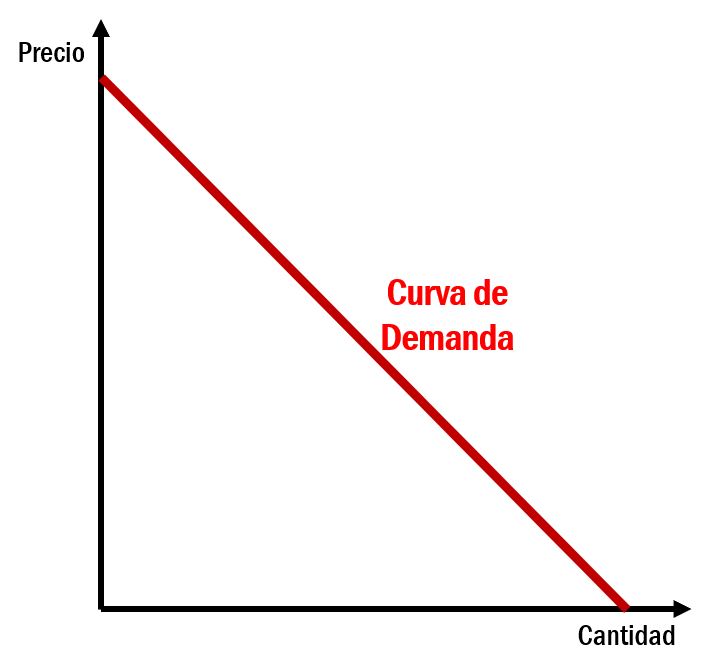
\includegraphics[width=0.5\linewidth]{images/12a-01} 

}

\caption{Curva de demanda}\label{fig:12a-01}
\end{figure}

La función de demanda es una relación matemática que recoge la relación entre la cantidad demandada de un bien, su precio y otras variables.

\hypertarget{movimientos-de-la-curva-de-demanda}{%
\subsection{Movimientos de la curva de demanda}\label{movimientos-de-la-curva-de-demanda}}

Cuando varía el precio de un bien, el desplazamiento se produce a lo largo de la curva de demanda Sin embargo, la curva de oferta se desplaza cuando se altera cualquiera de los factores que inciden en la demanda distinto del precio (Figura \ref{fig:12a-02}):

\begin{itemize}
\tightlist
\item
  La renta o ingreso de los consumidores (léase \emph{bienes normales} o \emph{bienes inferiores}).
\item
  Los precios de los bienes relacionados (léase \emph{bienes complementarios}, \emph{bienes sustitutivos} o \emph{bienes independientes}).
\item
  Los gustos o preferencias de los consumidores.
\item
  El tamaño del mercado o el número de consumidores.
\end{itemize}

\begin{figure}
\centering
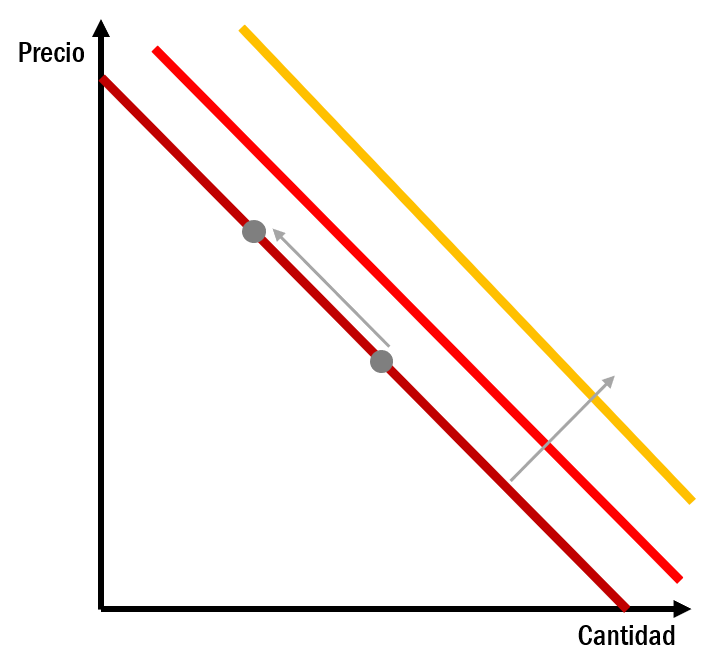
\includegraphics{images/12a-02.png}
\caption{\label{fig:12a-02}Movimientos a lo largo de la curva y de la curva de demanda}
\end{figure}

\hypertarget{la-oferta}{%
\section{La oferta}\label{la-oferta}}

La oferta es la cantidad que los productores (vendedores) quieren y pueden vender a los distintos precios.

\begin{quote}
\textbf{LEY DE LA OFERTA}:
Manteniéndose todo lo demas constante (\emph{ceteris paribus}), cuando aumenta el precio de un bien, la oferta aumenta.
\end{quote}

La oferta de mercado de un determinado bien es la suma de todas las oferta individuales que lo integran.

\hypertarget{la-curva-de-oferta}{%
\subsection{La curva de oferta}\label{la-curva-de-oferta}}

La curva de oferta (Figura \ref{fig:12a-03}) es la representación gráfica de la relación entre el precio de un bien y la cantidad ofrecida. Al trazar la curva de oferta suponemos que se mantienen constantes las demás variables, excepto el precio, que puedan afectar a la cantidad ofertada.

\begin{figure}
\centering
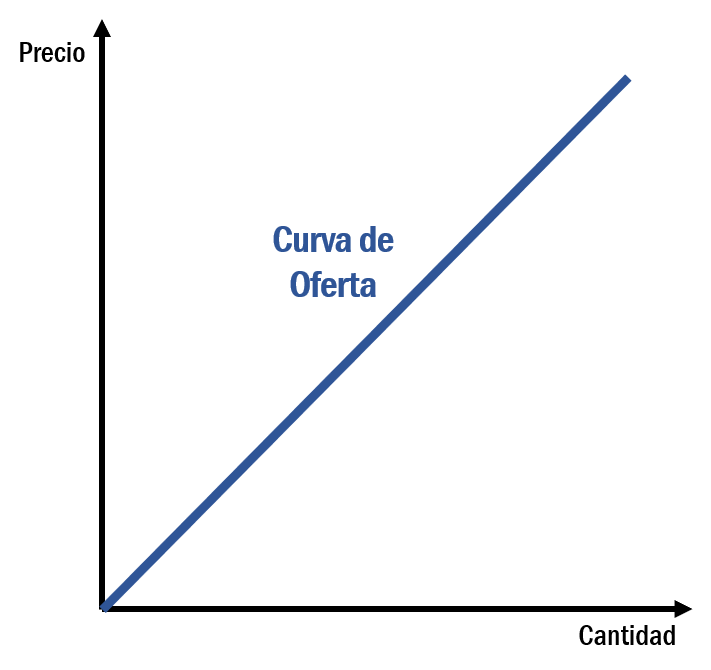
\includegraphics{images/12a-03.png}
\caption{\label{fig:12a-03}Curva de oferta}
\end{figure}

La función de oferta es una relación matemática que recoge la relación entre la cantidad demandada de un bien, su precio y las demás variables que influyen en las decisiones de producción.

\hypertarget{movimientos-de-la-curva-de-oferta}{%
\subsection{Movimientos de la curva de oferta}\label{movimientos-de-la-curva-de-oferta}}

Cuando varía el precio de un bien, el desplazamiento se produce a lo largo de la curva de oferta. Sin embargo, la curva de oferta se desplaza cuando se altera cualquiera de los factores que inciden en la oferta distinto del precio (Figura \ref{fig:12a-04}):

\begin{itemize}
\tightlist
\item
  El precio de los factores productivos.
\item
  La tecnología existente.
\item
  El número de empresas existentes en el mercado.
\end{itemize}

\begin{figure}
\centering
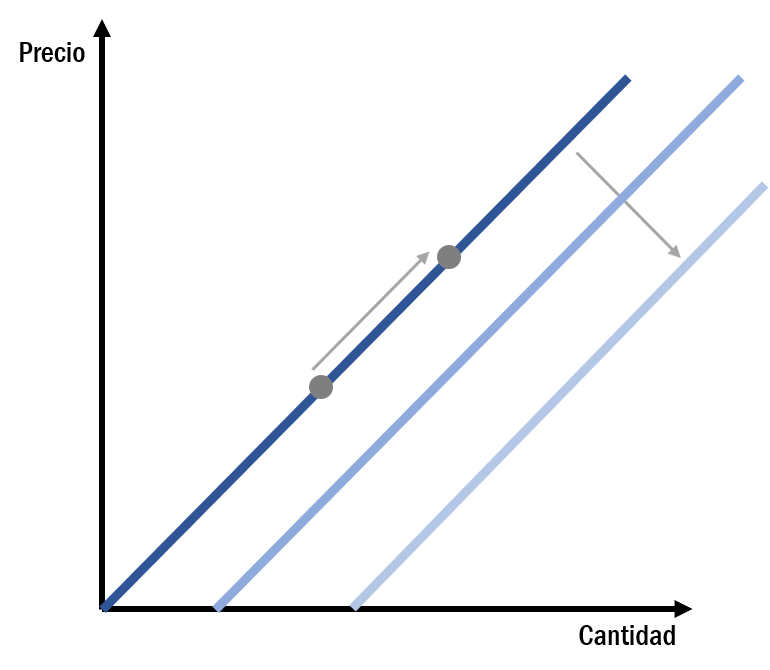
\includegraphics{images/12a-04.png}
\caption{\label{fig:12a-04}Movimientos a lo largo de la curva y de la curva de oferta}
\end{figure}

\hypertarget{el-punto-de-equilibrio}{%
\section{El punto de equilibrio}\label{el-punto-de-equilibrio}}

Cuando consumidores y productores se ponen en contacto para intercambiar un bien, cada uno de ellos con sus respectivas curvas de demanda y oferta, existe un punto en el que ambos agentes se ponen de acuerdo. Existen multitud de precios en los que los planes de cada uno de ellos no coinciden, pero existe un único punto en el que se da la coincidencia. Este es el punto de equilibrio del mercado y nos proporciona información sobre la cantidad (demandada y ofertada) y el precio de equilibrio.

\begin{quote}
\textbf{Punto de equilibrio}:
Es el punto en el que coinciden oferta y demanda. El precio de equilibrio es aquel en el cual la cantidad demandada es igual a la cantidad ofertada, siendo ésta la cantidad de equilibrio.
\end{quote}

\begin{figure}
\centering
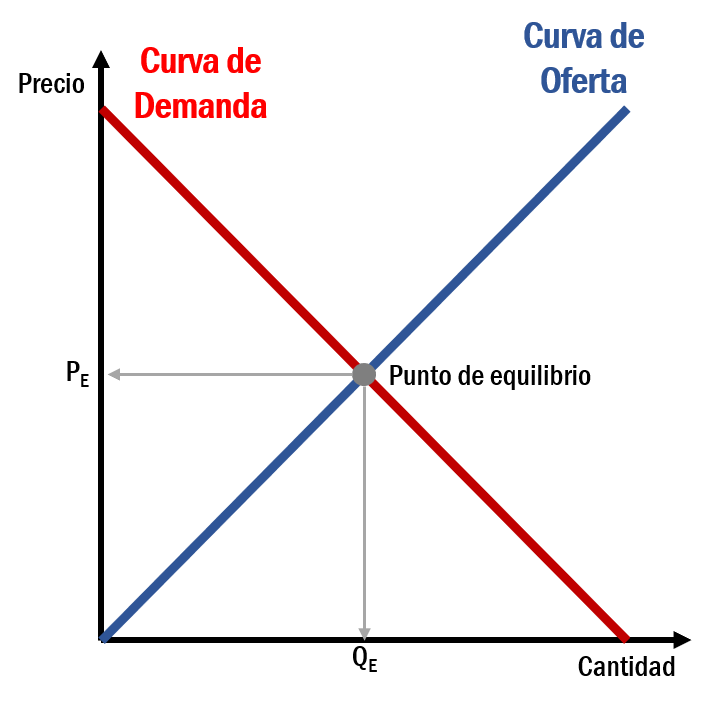
\includegraphics{images/12a-05.png}
\caption{\label{fig:12a-05}Punto de equilibrio entre la curva de oferta y la curva de demanda}
\end{figure}

En el punto de equilibrio, dado que los deseos de los consumidores y de los productores coinciden, no hay escasez ni excedente del bien.
Un exceso de oferta o excedente, es la situación en la que la cantidad ofrecida es mayor que la demandada.
Un exceso de demanda o escasez, es la situación en la que la cantidad demandada es mayor que la ofrecida.

Si a partir de una posición de equilibrio tienen lugar desplazamientos simultáneos de las curvas de demanda y de oferta, el impacto sobre el precio y la cantidad de equilibrio será ambiguo pues dependerá de la magnitud del cambio experimentado por cada una de las curvas.

\hypertarget{la-elasticidad}{%
\chapter{La elasticidad}\label{la-elasticidad}}

Para explicar el comportamiento de los consumidores podemos aceptar como punto de partida que los individuos tienden a elegir aquellos bienes y servicios que valoran más, es decir, aquellos que les reportan una mayor utilidad o satisfacción. En otras palabras, vamos a suponer que los individuos maximizan su utilidad, lo que implica que eligen el conjunto de bienes de consumo que más prefieren.

La utilidad es el sentimiento subjetivo de placer o satisfacción que una persona experimenta como consecuencia de consumir un bien o un servicio.

El principio equimarginal o de la igualdad de las utilidades marginales por euro gastado establece que cada bien se demanda hasta el punto en que la utilidad marginal del último euro gastado en él es exactamente igual a la utilidad marginal del último euro gastado en cualquier otro bien.

El excedente del consumidor de un bien es la diferencia entre la cantidad máxima que éste estaría dispuesto a pagar por el número de unidades del bien que demanda y la cantidad que realmente paga en el mercado. El excedente del consumidor es la diferencia entre la utilidad total de un bien y su valor total de mercado.

\hypertarget{elasticidad}{%
\section{Elasticidad}\label{elasticidad}}

La elasticidad es un concepto económico introducido por el economista inglés Alfred Marshall, para cuantificar la variación experimentada por una variable al cambiar otra. El concepto económico de la elasticidad parte de la existencia de dos variables, entre las que existe una cierta dependencia, por ejemplo el número de automóviles vendidos y el precio de los automóviles. La elasticidad mide la sensibilidad de la cantidad de automóviles vendidos ante la variación del precio de los mismos.

\hypertarget{elasticidad-de-la-demanda}{%
\section{Elasticidad de la demanda}\label{elasticidad-de-la-demanda}}

La elasticidad es una medida de la sensibilidad de la cantidad demandada o de la cantidad ofrecida ante el cambio en alguno de sus factores determinantes.

La demanda es elástica si la elasticidad precio de la demanda es mayor que 1; es inelástica si es menor que 1, y es de elasticidad unitaria si es igual a 1.

\hypertarget{elasticidad-de-la-oferta}{%
\section{Elasticidad de la oferta}\label{elasticidad-de-la-oferta}}

El concepto de elasticidad que se ha aplicado a la curva de demanda también puede referirse a la curva de la oferta.

La elasticidad es un indicador que nos sirve para medir los cambios de una variable cuando cambia otra. Hay dos tipos de elasticidad, segun: A)Precio de la demanda: Mide que es lo que sucede a la demanda cuando cambia el precio. B) Precio de la oferta: Mide los cambios en la oferta cuando varia el precio. Ambas varioaciones cuando son mayores que el 1\% se llaman elasticas, y cuando estan entre el 0 y 1\%, inelasticas.

\hypertarget{mercados}{%
\chapter{Mercados}\label{mercados}}

Un mercado es toda institución social en la que los bienes y servicios, así como los factores productivos, se intercambian. Permite una definición dual: desde un punto de vista puramente físico haciéndose referencia al lugar donde se producen los intercambios; desde un punto de vista más formal o institucional, hace referencia a la conjunción de compradores y vendedores.

Un mercado está compuesto por dos elementos fundamentales: por un lado la oferta, definida por la actitud de los productores; y por otro lado la demanda, determinada por el comportamiento de los consumidores.

Las principales caracteristicas que definen la estructura de un mercado son las siguientes:

\begin{enumerate}
\def\labelenumi{\arabic{enumi}.}
\tightlist
\item
  Numero de agentes.
\item
  Grado de competencia entre los vendedores.
\item
  Tipo de producto. Homogeneo o heterogeneo.
\item
  La existencia o no de barreras de entrada. Las cuales son el impedimento que hace que alguien no pueda entrar en un mercado. Dentro de estas distinguimos ciertos tipos:

  \begin{itemize}
  \tightlist
  \item
    Proceso productivo.
  \item
    Recursos monopolisticos.
  \item
    Patentes legales.
  \end{itemize}
\item
  Control sobre el precio.
\item
  La transparencia. Control sobre la información.
\end{enumerate}

En función de qué situaciones se den para cada una de las características anteriores, se distinguirá una tipología u otra de mercado. En general, se distinguen las siguientes tipologías básicas de mercados: competencia perfecta, monopolio, oligopolio y competencia monopolística.

\hypertarget{competencia-perfecta}{%
\section{Competencia perfecta}\label{competencia-perfecta}}

Los mercados de competencia perfecta se caracterizan porque presentan las siguientes características:

\begin{enumerate}
\def\labelenumi{\arabic{enumi}.}
\tightlist
\item
  Existencia de un número elevado de compradores y vendedores.
\item
  Existe una alta competencia entre los vendedores.
\item
  Los bienes ofrecidos por los distintos vendedores son prácticamente idénticos.
\item
  Las empresas pueden entrar o salir libremente del mercado.
\item
  Las empresas individualmente no tienen capacidad para fijar el precio del producto.
\item
  Existe información perfecta.
\end{enumerate}

\hypertarget{monopolio}{%
\section{Monopolio}\label{monopolio}}

Del griego antiguo mόνος (\emph{mono}, ``uno''), y de πόλλειν, (\emph{polein}, ``vender'').
El caso extremo de un mercado imperfectamente competitivo es el monopolio, ya que sólo hay un único ofertante en la industria. Una empresa es un monopolio si es la única que oferta un producto y si éste no tiene sustitutivos cercanos.

\begin{enumerate}
\def\labelenumi{\arabic{enumi}.}
\tightlist
\item
  Sólo existe un único vendedor.
\item
  No existe compentencia alguna al existir un único vendedor.
\item
  Se comercializa un único producto sin sustitutivos cercanos.
\item
  Generalmente aparecen importantes barreras de entrada al mercado.
\item
  El único vendedor tiene un gran poder a la hora de fijar el precio.
\item
  No existe una gran información sobre los costes del vendedor.
\end{enumerate}

Su objetivo principal es maximizar el beneficio. Encontramos que el precio del producto es mayor que el ingreso marginal
Ejemplos de monopolio son: el agua y las empresas de ferrocaril y autobuses.
Para este tipo de mercados hay diferentes soluciones como: aumentar la competencia y prohibir los monopolios.

\hypertarget{barreras-de-entrada}{%
\subsection{Barreras de entrada}\label{barreras-de-entrada}}

Las barreras a la entrada son factores que limitan la entrada de nuevas empresas en una industria, de forma que, cuando son altas, la industria tendrá pocas empresas y escasas presiones para competir.

\begin{enumerate}
\def\labelenumi{\arabic{enumi}.}
\tightlist
\item
  Las restricciones legales (patentes, las restricciones o concesiones administrativas, existencia de tarifas y cuotas al comercio internacional).
\item
  La publicidad y la diferenciación del producto.
\item
  Costes de entrada elevados.
\end{enumerate}

\hypertarget{oligopolio}{%
\section{Oligopolio}\label{oligopolio}}

Del griego antiguo ὀλίγος (\emph{oligos}, ``poco'', ``pocos''), y de πόλλειν, (\emph{polein}, ``vender'').

Este tipo de mercados esta caracterizado por tener pocos vendedores y muchos compradores, en el cual encontramos una gran competencia entre los vendedores e incluso encontramos pactos. Aqui las decisiones de un sujeto afectan a los demas, lo cual se llama: Interdependencia estrategica.
En estos mercados los vendedores deben elegir entre conseguir el maximo beneficio o cooperar con los demas vendedores. Al coopear encontramos dos tipos de pacto, el cartel, que es un grupo de empresas que trabajan como una sola, y la colusion, en la cual las empresas se reparten el mercado.
Un ejemplo de este mercado son los medicamentos.

\hypertarget{competencia-monopoluxedstica}{%
\section{Competencia monopolística}\label{competencia-monopoluxedstica}}

Las principales caracteristicas de este mercado es que la competencia entre los vendedores es alta dado que hay muchos, al igual que compradores que tambien hay muchos y las empresas tienen que competir por ellos. Podemos encontrar productos diferenciados y algun tipo de barrera al entrar a este mercado, como por ejemplo de tipo legal. Los vendedores tienen algo de control sobre el precio de sus productos y la transparencia es imperfecta.
Observamos algún ejemplo claro como los teléfonos móvil y los pañuelos de papel.

\hypertarget{otras-tipologuxedas}{%
\section{Otras tipologías}\label{otras-tipologuxedas}}

Así como en los monopolios y oligopolios hablábamos de la raíz griega πόλλειν, (\emph{polein}, ``vender''), podemos igualmente encontrarnos con monopsonios y oligopsonios. En este caso, aparece la raíz ψωνιος (\emph{psonios}, ``compra''), por lo que nos van a aparecer mercados en los que el poder lo tienen los compradores, bien porque sólamente hay uno (monopsonios) o porque hay muy pocos (oligopsonios).

Ejemplo de este tipo de mercados suele ser el sistema nacional de salud y su compra centralizada de medicamentos: un único comprador que engloba la compra de todos los medicamentos para el país, otorgando por tanto un poder importante a la hora de negociar el precio de compra. Cuando este sistema se transfiere a las comunidades autónomas, surgen distintos sistemas de salud encargados de realizar esta compra, por lo que se transforma el mercado en un oligopsonio. Los sistemas pierden algo de poder, pero al seguir siendo un número reducido, pueden seguir influyendo sobre el precio, y por supuesto, pueden agruparse para aumentar su poder al igual que sucedía en los oligopolios.

\hypertarget{los-fallos-de-mercado}{%
\chapter{Los fallos de mercado}\label{los-fallos-de-mercado}}

el funcionamiento de los mercados en ocasiones falla. Estos fallos de mercado se pueden sintetizar en la siguiente tipología:
A) Competencia imperfecta.
B) Externalidades.
C) Información imperfecta.

\begin{quote}
Un fallo del mercado tiene lugar cuando un mercado no asigna eficientemente los recursos por sí solo.
\end{quote}

\hypertarget{las-externalidades}{%
\section{Las externalidades}\label{las-externalidades}}

Aparecen externalidades, como la contaminación, que el mercado no aborda. Así, una industria que produce papel puede contaminar las aguas de un río al que vierte sus residuos. La actividad de la industria perjudica a los agricultores que utilizan el agua del río y los precios de producir papel no reflejan el perjuicio que se está ocasionando a los agricultores (véase Capítulo 8).

\hypertarget{competencia-imperfecta}{%
\section{Competencia imperfecta}\label{competencia-imperfecta}}

Existen mercados en los que la competencia es imperfecta. Como veremos en el Capítulo 6, en muchos mercados uno o más participantes pueden influir sobre los precios, fijando el nivel que les resulte más conveniente.

\hypertarget{informaciuxf3n-imperfecta}{%
\section{Información imperfecta}\label{informaciuxf3n-imperfecta}}

La información en muchos casos es imperfecta. En algunos mercados el supuesto de información plena está lejos de la realidad, lo que supone un fallo del mercado (véase Capítulo 8).

Este tipo de problemas sugiere la conveniencia de que en determinadas circunstancias el Estado pueda intervenir en la economía para tratar de mejorar su funcionamiento tanto a nivel de mercados concretos (esto es, vía políticas microeconómicas) como desde una perspectiva global, esto es, mediante el recurso a las políticas macroeconómicas. Por ello, en los países occidentales es frecuente hablar de economías mixtas.

\hypertarget{variables-macroeconuxf3micas}{%
\chapter{Variables macroeconómicas}\label{variables-macroeconuxf3micas}}

Hemos visto al inicio de estos apuntes que la microeconomía se ocupa del comportamiento de los agentes individuales (empresa, consumidor) y del funcionamiento de cada mercado. Por ejemplo, la determinación del precio y la cantidad producida de un bien y el estudio de los precios relativos son cometidos típicos de la microeconomía.

La macroeconomía, por el contrario, estudia el comportamiento del sistema económico en su conjunto (las magnitudes agregadas): la determinación de la producción total de un país, de los precios globales, del empleo, etc. Por ejemplo, la evolución general de todos los precios de la economía, una caída del empleo total en un país, o el efecto que un impuesto general sobre la renta de las personas pueda tener sobre la producción total de un país, serán problemas tratados por la macroeconomía. Mientras que la microeconomía analiza partes individuales de una economía, la macroeconomía se preocupa del conjunto.

Las principales variables de las que se ocupa la macroeconomía son aquéllas relativas a la producción agregada de un país (que correspondería a la agregación de todos los productos que se generan), el nivel general de precios (índice que representa los precios de todos los bienes) y el empleo total, entre otras magnitudes. La macroeconomía se fijará en la evolución de estas variables, de las posibles relaciones entre ellas y también de las fluctuaciones que puedan experimentar a lo largo del tiempo. Pero, antes de analizar su evolución es necesario conocer algo más sobre las magnitudes macroeconómicas. En primer lugar, estudiaremos cómo se agregan y se miden estas magnitudes y analizaremos su significado.

\hypertarget{renta-y-riqueza}{%
\section{Renta y riqueza}\label{renta-y-riqueza}}

El diagrama del Flujo Circular de la Renta nos enseña cómo se relacionan las empresas y los consumidores, y cómo a cambio de factores, los consumidores reciben lo que se denomina una renta. Estos factores pueden ser fuerza laboral (la capacidad de trabajar) pero también locales, medios de producción, activos financieros, etc, por lo que obtienen unas retribuciones adicionales. Así, definimos renta como la cantidad de dinero que recibe una persona por su contribución al mercado de factores.

La renta de una persona va a depender por tanto de los factores productivos que posea y ponga a disposición en el mercado, así como del precio que obtenga por ellos en el mercado. Las personas pueden decidir entre gastar esta renta en consumo (o inversión), o ahorrarla. En este segundo caso estarán generando riqueza.

La riqueza es el valor monetario de todos los bienes y derechos que posee una persona. Riqueza y renta están relacionadas. La riqueza la podríamos ver como el volumen de agua de una piscina, y la renta el agua del grifo que la llena. En función de la cantidad de renta que ingresemos podremos alcanzar un mayor o menor nivel de riqueza (siempre y cuando no tengamos el desagüe abierto).

\hypertarget{la-demanda-agregada-el-producto-interior-bruto}{%
\section{La demanda agregada: el Producto Interior Bruto}\label{la-demanda-agregada-el-producto-interior-bruto}}

El problema de la agregación para obtener las variables macroeconómicas se manifiesta con especial intensidad en el caso de la producción. Si se trata de medir la producción de un país durante un año determinado es necesario, en primer lugar, buscar una unidad de medida común para todos los bienes y servicios producidos. Es fácil observar que los distintos productos se miden en unidades diferentes: el arroz en toneladas, los automóviles en unidades, el vino en litros y los servicios en horas o en clientes atendidos. No se pueden sumar bienes heterogéneos que, además, se miden en unidades distintas.

La solución que se ha encontrado es agregar todos los bienes y servicios producidos a través de su valor de mercado. El valor de mercado de un producto se calcula multiplicando la cantidad producida de este bien por su precio de mercado. Una vez calculados los valores de mercado de todos los bienes y servicios de un país, que se expresarán en euros (u otra moneda), es posible agregar (sumar) todos ellos. La suma, que denominaremos producción agregada, se expresará también en unidades monetarias.

Este método de agregación concede un mayor peso en la suma total (decimos que pondera más) a aquellos bienes que tienen un precio superior. La justificación que se suele dar es que, en un sistema de mercados competitivos, los precios reflejan las preferencias de los consumidores. Por tanto, este método concede más importancia a aquellos bienes más valorados por los consumidores.

La medida más común de la producción agregada de un país es el Producto Interior Bruto (PIB), que se define como el valor de mercado de todos los bienes y servicios finales producidos durante un año en territorio nacional. Es importante analizar algunos elementos de esta definición con cierto detalle.

\begin{enumerate}
\def\labelenumi{\alph{enumi})}
\tightlist
\item
  El PIB se valora a precios de mercado, esto es, a través del precio que pagan los consumidores. Veremos más adelante que hay alguna otra forma de valorar los productos.
\item
  El PIB incluye tan sólo el valor de los bienes y servicios finales pero no el de los bienes y servicios intermedios que sirvieron para la fabricación de aquéllos. ¿Por qué no se incluyen los bienes intermedios? Porque el valor de estos bienes está ya incluido en el producto final. Si se sumase el valor de los bienes intermedios, se contaría dos veces su valor. Es el problema conocido como la doble contabilización.
\item
  El PIB se computa a lo largo de un año. La producción se va generando constantemente y debe ser medida a lo largo de un período de tiempo. Dicho de otro modo, el PIB es una variable flujo.
\item
  El PIB incluye sólo el valor de lo producido durante ese año. Si se vende ese año algo producido en otro año anterior, por ejemplo, un automóvil de segunda mano, el valor de esa venta no se incluirá en el PIB del año corriente. El motivo es que el valor de ese bien ya fue incluido en el PIB del año en que se produjo.
\item
  Se incluye en el PIB lo producido en el interior de un país, con independencia de que los factores que lo producen sean propiedad de nacionales o de extranjeros. Existen otras formas de medir la producción agregada (por ejemplo, el Producto Nacional Bruto), que utilizan otros criterios distintos.
\end{enumerate}

\hypertarget{la-comparaciuxf3n-entre-periodos.-pib-nominal-y-pib-real}{%
\subsection{La comparación entre periodos. PIB nominal y PIB real}\label{la-comparaciuxf3n-entre-periodos.-pib-nominal-y-pib-real}}

El PIB es un indicador de la actividad económica en un país que sirve, entre otras cosas, para conocer si la producción agregada del país en cuestión aumenta y, también, para medir a qué ritmo lo hace. Sin embargo, el hecho de que el PIB se agregue a través de los precios genera algunos inconvenientes cuando se utiliza para comparar entre dos períodos del tiempo distintos. Si se observa que de un año a otro el PIB ha crecido, este crecimiento puede deberse a dos causas:
a) Han aumentado las cantidades producidas de los bienes y servicios, o
b) Los productos se venden a precios superiores y, por ello, su valor ha aumentado.
Lo más común es que, de un año a otro cambien tanto las cantidades producidas como los precios. Para separar estos dos efectos, los economistas distinguen entre el PIB nominal y el PIB real.

Cuando tenemos una serie de valores del PIB para años diferentes, definimos el Producto Interior Bruto nominal como aquél en el que se ha agregado la producción total del país utilizando los precios del año en el que se produjo cada bien o servicio. Por ello, esta magnitud se conoce también como PIB a precios corrientes. Las variaciones del PIB nominal pueden deberse tanto a cambios de las cantidades producidas como de los precios.

Por su parte, se define el Producto Interior Bruto real como aquél que se agrega utilizado los mismos precios para todos los períodos. Estos precios son los de un año cualquiera que se toma como base para el cálculo. Por ello, esta magnitud se conoce también como PIB a precios constantes, ya que está expresada en unidades monetarias constantes de un año base. Como el PIB real se calcula utilizando siempre los mismos precios, sus variaciones se deben sólo a cambios en las cantidades producidas de los bienes.

Uno de los indicadores más utilizados de la evolución de la actividad económica de un país es la tasa de crecimiento del PIB, que se define como el incremento porcentual del PIB real durante un año.

Las tasas de crecimiento se pueden calcular también para el PIB nomina, pero entonces el significado es distinto, ya que estas tasas recogerían la variación de los precios. No obstante, cuando se habla de crecimiento de la economía o crecimiento de la producción en general se está haciendo referencia a la tasa de crecimiento del PIB real.

Muchas veces resulta interesante conocer en cada país la cantidad que se produce por persona. Para ello se utiliza el PIB per capita, que se calcula como el cociente entre el PIB de un país y su número de habitantes. El PIB per capita representaría el valor del producto que correspondería a cada habitante si la producción se repartiera equitativamente.

\hypertarget{enfoques-para-obtener-el-pib}{%
\subsection{Enfoques para obtener el PIB}\label{enfoques-para-obtener-el-pib}}

Hasta este momento hemos medido el Producto Interior Bruto de un país a partir del valor de la producción de todos los bienes y servicios generados. Es lo que vamos a denominar el enfoque del valor de la producción. Sin embargo, el PIB refleja otros dos aspectos macroeconómicos que son el gasto total y las rentas o ingresos totales. Dicho de otro modo, el PIB puede medirse también como el gasto total que se realiza en un país o como la suma de todas las rentas o ingresos en el país. Vamos a analizar estos dos últimos enfoques haciendo especial insistencia en que todos los criterios llegan al mismo resultado.

Los bienes y servicios que se producen en un país salen al mercado y son comprados por los agentes económicos. Por tanto, podemos medir también el valor de la producción a través del gasto agregado efectuado por los compradores de estos bienes o servicios. Parece evidente que, en todo intercambio, el valor de lo que se vende debe coincidir con el desembolso del comprador. Por ello, el PIB también mide el gasto agregado de un país. Este segundo método para medir el PIB se conoce como el enfoque del gasto.

Sin embargo, todavía hay otra forma de medir la el PIB que se denomina enfoque de las rentas o de los ingresos. En el intercambio de mercado, lo que es un gasto para una persona supone un ingreso para otra. Por tanto, el gasto total en la economía debe coincidir con la suma total de rentas o ingresos de todos los participantes. También podemos verlo de otro modo. El valor de un producto, una vez vendido, se reparte entre las personas que aportaron los factores productivos utilizados (salarios a los trabajadores, alquileres a los que aportaron el local, beneficio para el empresario, etc.). Por tanto, si sumamos todas las empresas, concluimos que el valor de la producción total de un país se reparte, en forma de rentas o ingresos, entre los que han participado en esta producción. Por tanto, el PIB también puede medirse como la suma total de rentas o ingresos que se generan en los procesos productivos de un país (salarios, alquileres, intereses, beneficios, etc.).

\hypertarget{el-nivel-de-precios}{%
\section{El nivel de precios}\label{el-nivel-de-precios}}

Una de las informaciones que más interesa a los ciudadanos, ya sean amas de casa, trabajadores, pensionistas e incluso estudiantes de economía, es la relativa al crecimiento de los precios. No resulta tarea sencilla medir lo que aumentan los precios durante un determinado período de tiempo, ya que no basta con observar su evolución. Los bienes y servicios que compran los consumidores son muchos y muy variados; si alguien preguntase al economista ¿cuánto han subido «los precios» durante este año?, el primer impulso podría consistir en responder con otra u otras preguntas: ¿qué precios?, ¿el de la carne?, ¿el del pescado?, ¿el del pan?, ¿el de la gasolina? Sin embargo, es evidente que el interlocutor no está interesado en la variación del precio de ningún artículo concreto sino en la evolución de los precios «en general». Es necesario, por ello, obtener una magnitud que represente a todos los precios. El problema estriba en la manera de hacerlo.

\hypertarget{el-uxedndice-de-precios-de-consumo}{%
\subsection{El Índice de Precios de Consumo}\label{el-uxedndice-de-precios-de-consumo}}

El Índice de Precios de Consumo (IPC) es la medida del nivel de precios más utilizada. Como su propio nombre indica, engloba, tan sólo, los precios de los bienes y servicios de consumo final, que compran las familias en un país, pero no los precios de los bienes de capital ni de los bienes intermedios. Por su carácter de índice, tiene la propiedad de tomar el valor 100 en un período del tiempo arbitrario, que se toma como base y que sirve como punto de referencia para los demás períodos. El IPC se ha calculado tradicionalmente a través de una fórmula conocida como Índice de Laspeyres convencional con los siguientes pasos:

\begin{enumerate}
\def\labelenumi{\arabic{enumi}.}
\tightlist
\item
  Se toma un año como base y, en ese año, se mide el porcentaje del gasto de la familia media en cada uno de los bienes. Estos porcentajes se utilizarán como ponderaciones para calcular el IPC en el resto de los períodos.
\item
  Se mide el precio de cada producto en todos los años en los que se desea calcular el IPC, incluyendo el año base.
\item
  Se calcula el IPC como una media ponderada de los cocientes, para cada producto, entre el precio en el año en cuestión y el precio de ese producto en el año base.
\end{enumerate}

\hypertarget{el-deflactor-del-pib}{%
\subsection{El deflactor del PIB}\label{el-deflactor-del-pib}}

El IPC no es la única manera de medir el nivel general de precios. Se estudió anteriormente la diferencia entre el Producto Interior Bruto (PIB) nominal y el PIB real. Mientras que el primero se calculaba agregando los valores de los bienes medidos según los precios de cada año, el segundo se obtenía valorando los bienes según los precios de un año que se tomaba como base. Por tanto, las diferencias que se pueden observar entre el PIB nominal y el PIB real se deben a las variaciones de los precios entre el año base y el año corriente. Es posible utilizar el cociente entre estas dos magnitudes como una medida del nivel general de precios que se conoce como deflactor del PIB.
\[\mathrm {\text{Deflactor del PIB} = \frac{\text{PIB nominal (año t)}}{\text{PIB real (año t)}}·100}\]
El deflactor del PIB es un índice de precios que toma el valor 100 en el año base y será tanto más elevado en el año «t» cuanto mayor haya sido el incremento de los precios entre el año 0 (año base) y el año t.

Aunque los dos son índices que miden los precios agregados de un país, existen algunas diferencias entre el IPC y el deflactor del PIB.

La primera diferencia es que el IPC tan sólo incluye los precios de los bienes que se consumen mientras que el deflactor del PIB incluye los precios de todos los bienes y servicios que se producen en el país. Por tanto, los precios de los bienes de capital (maquinaria, etc.) producidos en un país forman parte del deflactor del PIB, pero no se incluyen en el IPC.

La segunda diferencia consiste en que los precios de los bienes de consumo importados se incluyen en el IPC, dado que los consumidores de un país los compran, pero no se computan en el deflactor del PIB al no ser producidos en el país.

La tercera diferencia consiste en que el IPC, medido como un índice de Laspeyres convencional, pondera los precios según el consumo de un año base mientras que el deflactor del PIB pondera los precios según la producción de cada año. Obviamente esta diferencia es mucho menor si se utiliza el Índice de Laspeyres encadenado para calcular el IPC.

¿Cuál de los dos índices de precios es más conveniente? Depende de lo que se desee medir. El IPC es más adecuado para determinar cuánto suben los precios para los individuos o las familias, dado que estos compran básicamente bienes de consumo. Para estudiar si los productos de un país se están encareciendo o no con respecto a los del extranjero puede ser más adecuado el deflactor del PIB.

\hypertarget{el-mercado-de-trabajo}{%
\section{El mercado de trabajo}\label{el-mercado-de-trabajo}}

La macroeconomía se ocupa también de estudiar las magnitudes agregadas relativas al nivel de empleo del factor trabajo. Estas variables guardan relación con aquéllas que se refieren a la producción, ya que a mayor nivel de empleo del factor trabajo mayor nivel de producción.

Para analizar las variables relativas al empleo se clasifica la población de un país tal como lo hace la Figura 10.3.

\begin{itemize}
\tightlist
\item
  La población en edad de trabajar está formada por todas las personas que han alcanzado la edad legal para poder trabajar (en España, por ejemplo, la edad está fijada en 16 años).
\item
  La población en edad de no trabajar está formada por aquéllos que no han alcanzado la edad legal para poder trabajar.
\item
  La población activa está formada por aquellas personas en edad de trabajar que han decidido dedicarse a una actividad remunerada en el mercado.
\item
  La población inactiva está formada por las personas en edad de trabajar que han decidido, en ese momento, no dedicarse a una actividad remunerada sino a otras actividades. Ejemplos de
  población inactiva son los estudiantes o las amas de casa o los jubilados. Es importante observar que formar parte de la población activa o inactiva constituye, en muchas ocasiones, una decisión voluntaria por parte de los individuos.
\item
  Los ocupados o empleados son aquellas personas que forman parte de la población activa y que logran encontrar un empleo.
\item
  Dentro de la población activa, hay otros que no encuentran empleo, aunque lo buscan, y se denominan desempleados.
\item
  De los ocupados, unos trabajan para otras personas (asalariados o trabajadores por cuenta ajena) y otros para sí mismos (trabajadores por cuenta propia o autónomos).
\end{itemize}

Es importante señalar, atendiendo a la clasificación de variables flujo y fondo que se desarrolló al principio del capítulo, que tanto el número de desempleados como el de activos o de ocupados son variables fondo.

Por otro lado, existen dos indicadores muy importantes del nivel de empleo, que son la tasa de actividad y la tasa de desempleo.

\begin{enumerate}
\def\labelenumi{\alph{enumi})}
\tightlist
\item
  La tasa de actividad es el porcentaje que representa la población activa dentro de la población en edad de trabajar.
\end{enumerate}

\[\mathrm {\text{Tasa de actividad} = \frac{\text{Población activa}}{\text{Población en edad de trabajar}}·100}\]

\begin{enumerate}
\def\labelenumi{\alph{enumi})}
\setcounter{enumi}{1}
\tightlist
\item
  La tasa de desempleo mide el porcentaje que representan los desempleados dentro de la población activa.
\end{enumerate}

\[\mathrm {\text{Tasa de desempleo} = \frac{\text{Desempleados}}{\text{Población activa}}·100}\]

\hypertarget{el-dinero}{%
\chapter{El dinero}\label{el-dinero}}

\hypertarget{quuxe9-es-el-dinero}{%
\section{¿Qué es el dinero?}\label{quuxe9-es-el-dinero}}

Definimos dinero como todo activo o bien que es generalmente aceptado como medio de pago por los agentes económicos para sus intercambios.

Es posible admitir una segunda definición: ``conjunto de activos que se encuentras dentro de una economía y que las personas usan regularmente para intercambiar bienes y servicios''.

Para comprender mejor estas definiciones, puede ser una buena idea ver cómo surge el dinero y cuáles son sus principales funciones y características.

\hypertarget{historia-del-dinero}{%
\section{Historia del dinero}\label{historia-del-dinero}}

Retrocedamos en el tiempo, hasta el neolítico (1900 años a.C.). En aquella época aparecen la agricultura y la ganadería, y con su desarrollo apareció la primera economía de producción y se produjeron los excedentes, es decir, bienes que no necesitan ser consumidos. Esto dio lugar a la posibilidad de alimentar a personas que no necesitaban trabajar la agricultura o la ganadería y podían dedicarse a producir otros productos, como la cerámica o la caza. Con esos excedentes se producía un intercambio de productos. Este intercambio supuso la aparición de la primera forma de comerciar, el trueque, intercambiando directamente bienes y servicios por otros.

El dinero aparece más tarde en la antigüedad remota como una forma de superar los problemas que acarreaba el trueque o intercambio directo de unas mercancías por otras. A medida que las economías se vuelven más complejas y el número de bienes se multiplica, es cada vez más difícil que se verifique la coincidencia de deseos de las dos partes que intervienen en el intercambio si éste se realiza en forma de trueque. Si sólo existen dos bienes, resulta relativamente fácil que una persona que desea intercambiar el bien 1 (comida) por el bien 2 (vestido) encuentre a otra que desee intercambiar el bien 2 (vestido) por el bien 1 (comida). Pero si hay 100 bienes, resulta difícil que una persona que desea intercambiar el bien 71 (arroz) por el bien 29 (una oveja) encuentre a una persona que desee lo contrario.

Además, existe la dificultad de valorar los bienes que se van a intercambiar. ¿Cuántas ovejas cambio por un kilo de arroz? ¿Y qué sucede si los bienes no son divisibles? ¿Cómo consigo un vestido si yo me dedico a construir casas? Tendría que recibir 500 vestidos cuando yo en realidad sólo necesito uno. ¿Qué hago con los 499 restantes? No sólo es necesaria la coincidencia de necesidades, sino que en el trueque es muy complicado medir exactamente cuánto vale cada bien comparado con el otro.

Solución: todos aceptan cambiar cualquier bien por uno que previamente se ha fijado, por ejemplo, la sal. A este último bien se le denomina dinero mercancía. Ahora se puede cambiar el arroz por sal a una persona para posteriormen- te intercambiar esa cantidad de sal por una oveja a otra persona distinta. La sal se ha convertido, en este ejemplo, en el dinero (de hecho se utilizó en la antigüedad como dinero), ya que es el medio de cambio generalmente aceptado. También es muy probable que todos los precios comiencen a expresarse en unidades de sal (unidad de cuenta). Por otro lado, este método permite que el vendedor del arroz guarde la sal durante ese año y compre la oveja el año siguiente aplazando así la transacción (sirve como depósito de valor). Como curiosidad, se dice que la palabra «salario» proviene de «sal» dado que en la antigua Roma se realizaban algunos pagos en esta mercancía por la prestación de ciertos servicios. En definitiva, el dinero mercancía se caracteriza por tener un valor intrínseco o material que coincide con el valor que representa. Además de la sal, otros bienes como el tabaco, la plata y, sobre todo, el oro fueron utilizados como dinero mercancía. Se trataba de bienes que resultasen relativamente escasos (para mantener su valor), no perecederos, de alguna manera divisibles (para facilitar el cambio) y no muy voluminosos. En el caso del oro, y con el fin de garantizar la pureza del material (evitando así a los vendedores tener que comprobar la calidad) las autoridades comenzaron a acuñarlo (distribuirlo en porciones con el sello del monarca o la autoridad feudal) en forma de monedas que expresaban un determinado valor. Como la característica fundamental del dinero mercancía era que su valor material coincidía con el valor que representaba, era posible comprar la misma cantidad de bienes con la moneda de oro que fundiendo la moneda e intercambiando el metal resultante.

A pesar de todo, el oro resultaba un dinero incómodo por el elevado peso del metal. La gente comenzó a percatarse de que podía mantener el oro depositado en alguna institución o persona que garantizase su seguridad y pagar con un papel canjeable por una determinada cantidad de oro. Estos depositarios de oro se convertirían con el tiempo en bancos. El receptor del papel podía pagar también con él en lugar de hacerlo efectivo: había nacido el dinero fiduciario que se caracteriza porque su valor material (papel) es muy inferior a lo que puede comprar. Pronto las autoridades emiten ese papel (billetes) como una promesa de pago en oro (dinero legal). Todas las personas aceptaban este dinero legal porque sabían que en cualquier momento podían ir al depositario y canjearlo por oro (el oro era el activo que, en aquellos tiempos, respaldaba al dinero legal). Además, las autoridades comenzaron a promulgar leyes y disposiciones que establecían la obligatoriedad de aceptar este dinero como cobro de deudas. Naturalmente que la cantidad de papel moneda que se podía emitir estaba limitada por las disponibilidades de oro.

Tiempo después las autoridades anulan la convertibilidad deldinero legal en oro y comienzan a respaldar el dinero con otros activos distintos (por ejemplo, créditos a entidades, títulos financieros, moneda extranjera, etc.), como se verá más adelante. Si los billetes ya no son canjeables por oro, ¿por qué se siguen aceptando en el intercambio? Por dos motivos. El primero de ellos es que existe una obligación por ley de aceptarlos. El segundo, y más importante, por una cuestión de confianza, ya que aceptamos que nos paguen con billetes porque confiamos en que nos aceptarán estos mismos billetes en una compra posterior. Así, la palabra fiduciario significaría «basado en la confianza». Cuando, en deter- minadas situaciones históricas, los ciudadanos pierden confianza en su moneda, ésta deja de tener alguna de las propiedades que se atribuyen al dinero.

Hoy día las cosas son todavía más complicadas. La mayor parte de las transacciones de cierta entidad no implican intercambio alguno de monedas y billetes (se paga con tarjetas, transferencias bancarias, cheques, etc.) sino meros apuntes en unas cuentas abiertas en entidades de crédito (bancos, cajas de ahorros, etc.). Se llevan a cabo a través del dinero bancario, que está formado por las cuentas o depósitos que los particulares abren en los bancos. Estas cuentas tienen, desde el punto de económico, unas características parecidas a las de las monedas y billetes y pueden servir para realizar pagos. Por ello se consideran también dinero. Hoy día la cantidad total de dinero está formada por dinero legal y dinero bancario.

\begin{quote}
TIPOS DE DINERO

\begin{itemize}
\tightlist
\item
  \textbf{Dinero mercancía}: su valor intrínseco coincide con su valor
  representativo.\\
\item
  \textbf{Dinero fiduciario}: su valor intrínseco es inferior a su valor representativo.

  \begin{itemize}
  \tightlist
  \item
    Dinero legal: monedas y billetes.\\
  \item
    Dinero bancario: cuentas o depósitos en bancos, que
    sirven para realizar pagos.
  \end{itemize}
\end{itemize}
\end{quote}

\begin{center}\rule{0.5\linewidth}{0.5pt}\end{center}

\hypertarget{funciones-y-caracteruxedsticas}{%
\section{Funciones y características}\label{funciones-y-caracteruxedsticas}}

El dinero cumple tres funciones básicas:

\begin{itemize}
\tightlist
\item
  Medio de cambio, porque es intercambiable por otros bienes y servicios. Esta función es la principal y anula el trueque. Permite comprar bienes y servicios porque todo el mundo lo acepta como forma de pago. Éste es uno de los motivos por el que las personas mantienen una parte de su riqueza en forma de dinero aunque con ello no obtengan rentabilidad alguna.
\item
  Unidad de cuenta, porque determina el precio de cualquier bien en función de una cantidad de dinero.
\item
  Depósito de valor, debido a que podemos ahorrar dinero para conservar riqueza. Si no se desea consumir hoy lo ganado, es posible mantener el ahorro en forma de dinero aplazando la compra al futuro.
\end{itemize}

Para poder denominar a un activo dinero, debemos asegurarnos que cumpla sus principales características:

\begin{itemize}
\tightlist
\item
  Aceptabilidad. Una de las razones por las que el dinero funciona en el desempeño de sus funciona es porque es universalmente aceptado por la sociedad y los agentes económicos. Si un bien no es aceptado como dinero, no permite el intercambio de bienes y servicios y por tanto, el funcionamiento del comercio.
\item
  Durabilidad. Si el dinero no fuera duradero y resistente al paso del tiempo, no serviría como depósito de valor y podría además dañarse en los intercambios, perdiendo valor.
\item
  Transferibilidad. El dinero debe facilitar el intercambio y el comercio. Si no es fácil de usar y transportar, pierde gran utilidad.
\item
  Divisibilidad. Una de las razones por las que surge el dinero es por la necesidad de fraccionar los bienes que intervienen en las transacciones. El dinero debe ser fraccionable para facilitar el intercambio.
\item
  Homogeneidad. Cualquier unidad del dinero debe tener un valor exactamente igual al de las demás.
\item
  Dificultad de producción. Debe de ser difícil de producir y de falsificar.
\item
  Estabilidad. Su valor no debe de estar sujeto a fluctuaciones violentas.
\end{itemize}

\hypertarget{el-dinero-como-activo}{%
\section{El dinero como activo}\label{el-dinero-como-activo}}

Un activo es cualquier forma de mantener la riqueza. El dinero es, naturalmente, un activo (se puede mantener la riqueza en forma de dinero) pero no es el único. Los activos se dividen en reales y financieros. Los activos reales son aquellos materiales y tangibles: edificios, tierras, maquinaria, medios de transporte, viviendas, etc. Los activos financieros no son tangibles. Son documentos en los que personas o instituciones reconocen una deuda con el poseedor.

Estos documentos constituyen un pasivo para el que lo emitió (debe esa cantidad), pero un activo para el que lo posee (le deben esa cantidad). Ejemplos de activos financieros son: las letras de cambio, las acciones, las obligaciones, los títulos de la deuda pública, las cuentas bancarias o las monedas y billetes. Especial atención merecen estos dos últimos activos.

Los billetes de curso legal constituyen un activo financiero distinto de las cuentas bancarias o depósitos si bien resulta muy sencillo convertir uno en el otro: ingresando en efectivo los billetes en un banco, el individuo está cambiando sus activos de billetes a depósitos. Por el contrario, cuando el individuo se persona en la ventanilla del banco o en el cajero automático para solicitar billetes, está cambiando depósito por billetes. En el lenguaje cotidiano ambos activos se denominan dinero; más adelante se verá que ambos activos son distintos tipos de dinero. Por tanto, el dinero es un activo financiero, se trate éste de billetes o de depósitos. Los billetes representan una deuda de quien los emitió (ya veremos que el Banco Central) con las personas que los poseen. Una cuenta bancaria es un depósito que un particular realiza en un banco. Mediante este instrumento, el banco reconoce la deuda con el particular y le ofrece una serie de servicios relacionados como puede ser la realización de pagos y cobros. El resto de los activos que poseen los individuos pueden convertirse en dinero: por ejemplo, pueden venderse en la bolsa las acciones que se poseen. ¿En qué se diferencian unos activos de otros? Los activos se diferencian entre sí y se clasifican según su liquidez, su riesgo y su rentabilidad.

La liquidez mide la facilidad con la que un activo puede convertirse en dinero sin incurrir en costes o pérdidas. Un inmueble es un activo poco líquido, mientras que los billetes son pura liquidez. La rentabilidad es el interés que ofrece el activo, es decir, lo que se puede ganar por cada euro asignado a ese activo. Existen activos que pueden ser muy rentables (por ejemplo, las acciones), otros muy poco rentables (las cuentas bancarias), mientras que de las monedas y billetes no puede obtenerse rentabilidad.

El riesgo mide la inseguridad de un activo para recuperar lo asignado a él y su rendimiento. Las monedas y billetes tienen bajo riesgo, aunque no nulo. Si se mantiene una buena parte de la riqueza en forma de billetes, se corre el riesgo de sufrir un robo o, tal como vimos en su momento, una pérdida de poder adquisitivo debido a la inflación. Por el contrario, las acciones son activos bastante arriesgados, ya que su valor está sujeto a grandes oscilaciones.

Haciendo una clasificación de los activos, los más líquidos también suelen ser los menos arriesgados y los menos rentables. Por el contrario, los menos líquidos son también los más arriesgados y más rentables. Esta relación directa que existe en los activos financieros entre riesgo y rentabilidad (a mayor riesgo, mayor rentabilidad media) se explica como una consecuencia de la aversión al riesgo de los agentes económicos, que consiste en que a las personas no les gusta el riesgo. Si la rentabilidad de los activos más seguros fuese la misma que la de los activos más arriesgados, nadie mantendría estos últimos. Por tanto, los activos más arriesgados deben ofrecer una rentabilidad media superior (una prima de riesgo) para que las personas los adquieran.

\hypertarget{la-creaciuxf3n-de-dinero}{%
\section{La creación de dinero}\label{la-creaciuxf3n-de-dinero}}

Si todo el dinero utilizado se limitase a monedas y billetes de curso legal, la cantidad de dinero en circulación estaría constituida por lo que se denomina base monetaria. La base monetaria es el conjunto de los pasivos monetarios de un Banco Central (básicamente billetes que han sido emitidos). En el pasado era el oro el activo que respaldaba esta base monetaria. Hoy en día, los billetes están respaldados por otros activos distintos aunque los bancos centrales continúen manteniendo una cierta cantidad de oro.

Sin embargo, hoy en día, el grueso del volumen de transacciones se realiza a través de métodos que no requieren el intercambio de monedas y billetes: se paga con tarjetas, cheques, transferencias bancarias, etc. ¿En qué consisten estas nuevas formas de pago? Se trata, sencillamente, de apuntes contables que realizan unos agentes económicos denominados bancos comerciales privados. Los bancos son empresas que intermedian en los mercados financieros
canalizando fondos de los ahorradores a los particulares y empresas que utilizan dicho ahorro. Las personas realizan depósitos en los bancos (también conocidos como cuentas) y éstos utilizan esos recursos para conceder créditos o préstamos a quien lo solicita.

Un depósito es una anotación (en euros o en otra moneda) que refleja la deuda que el banco contrae con el titular. Se trata, por tanto, de un pasivo para el banco y un activo para el individuo. Los depósitos son activos muy líquidos, ya que resulta sencillo y rápido convertirlos en monedas y billetes: basta con acercarse a la ventanilla del banco o al cajero automático. Una de las características importantes de estos depósitos es que, además de servir para mantener la riqueza, se pueden utilizar para realizar pagos. Las tarjetas, cheques o transferencias no son más que ordenes para modificar el estado de las cuentas o depósitos. Si dos personas tienen la cuenta en el mismo banco, la primera puede pagar a la segunda ordenando una transferencia. El banco realiza la transferencia anotando apuntes que consisten en una reducción (cargo) de la cuantía de la cuenta de la primera persona y un aumento (abono) de la cuantía de la cuenta de la segunda persona. Si cada persona tiene cuenta en un banco distinto el procedimiento es el mismo, la única diferencia es que los bancos compensarán entre sí esta transferencia mediante apuntes en las cuentas que los bancos tienen abiertas, a su vez, en el Banco Central.

Dado que estos depósitos o cuentas sirven para realizar transacciones sin que medie intercambio de monedas y billetes, cumpliendo así una función similar a la de éstos últimos, los depósitos de los particulares en los bancos se consideran dinero. En realidad se trata de otra forma de dinero que, al ser creada por los bancos, se denomina dinero bancario. Los depósitos o dinero bancario son creados por los bancos comerciales en un proceso en el que, a partir del dinero legal (monedas y billetes), se crea una cantidad de dinero que supera, con creces los billetes existentes.

¿Cómo se crea esta nueva cantidad de dinero? Cuando depositamos dinero en nuestra cuenta bancaria, el banco, buscando obtener un beneficio, puede prestar todo ese dinero o parte de él. Imaginemos que tenemos 1.000 euros, y que depositamos en nuestra cuenta del banco 850 euros (el resto nos lo quedamos en el bolsillo para poder gastarlo). De los 850 euros que depositamos, el banco guarda un porcentaje en su caja (para mantener una cierta liquidez por si fuera necesaria, por ejemplo, si vamos a sacar dinero al cajero) y el resto lo presta a otro cliente. Supongamos que presta 800 euros de los 850. Ese nuevo cliente tiene ahora en su poder 800 euros, que sumados a nuestros 1.000 euros implica que la cantidad total de dinero circulando en la economía es de 1.800 euros. Esto no quiere decir que los sujetos seamos más ricos: nosotros seguimos teniendo 1.000 euros, y el otro cliente tiene que satisfacer una deuda. Sin embargo sí que ha aumentado la cantidad de dinero circulando y el banco ha creado una mayor liquidez.

En teoría este proceso se puede repetir infinitamente. El cliente puede volver a depositar el dinero prestado en otro banco, que a su vez podría volver a prestarlo, etc. En la zona euro, el Banco Central Europeo (BCE) determina como medida de prudencia económica que las entidades depositen un porcentaje de los depósitos de sus clientes en el banco central de cada país en concepto de reservas. Este porcentaje es lo que se denomina coeficiente de caja o coeficiente de reservas. Su finalidad es garantizar la solvencia a corto plazo de los bancos, impidiendo la multiplicación de fondos de un modo descontrolado que pudieran provocar quiebras en el sistema.

\hypertarget{el-crecimiento-y-los-ciclos-econuxf3micos}{%
\chapter{El crecimiento y los ciclos económicos}\label{el-crecimiento-y-los-ciclos-econuxf3micos}}

La expansión de las posibilidades de producción es el crecimiento económico. Un rápido ritmo de crecimiento económico sostenido a lo largo de cierto número de años puede transformar a una nación pobre en rica. Ésa ha sido la experiencia de Hong Kong, Corea del Sur y otras economías asiáticas. Un crecimiento económico lento o nulo pueden llevar a un país a una pobreza devastadora. Tal ha sido la suerte de Sierra Leona, Somalia, Zambia y buena parte del resto de África.

El objetivo de este capítulo es ayudarle a entender por qué algunas economías se expanden rápidamente mientras que otras se estancan. Comenzaremos por aprender cómo calcular una tasa de crecimiento; además, distinguiremos entre crecimiento económico y expansión del ciclo económico, y descubriremos los beneficios del crecimiento sostenido.

\hypertarget{cuxe1lculo-de-tasas-de-crecimiento}{%
\section{Cálculo de tasas de crecimiento}\label{cuxe1lculo-de-tasas-de-crecimiento}}

Expresamos la tasa de crecimiento como el cambio porcentual anual de una variable; esto es, el cambio en el nivel de ésta, expresado como porcentaje de su nivel original. La tasa de crecimiento del PIB real, por ejemplo, se calcula como:
\[\mathrm {\text{Tasa de crecimiento del PIB real} = \frac{\text{PIB real (año t) PIB real (año t-1)}}{\text{PIB real (año t)}}·100}\]
Empleando algunos números, si el PIB real en el año en curso es de 11 billones de dólares, y si el PIB real en el año anterior fue de 10 billones, entonces la tasa de crecimiento económico es del 10 por ciento.

La tasa de crecimiento del PIB real nos indica cuán rápidamente se está expandiendo la economía total. Esta medida es útil para conocer los cambios que podrían darse en cuanto al equilibrio del poder económico entre las naciones. Sin embargo, no nos dice nada respecto de los cambios ocurridos en el estándar de vida.

El estándar de vida depende del PIB real per cápita, que es el PIB real dividido entre la población. Por consiguiente, la contribución del incremento del PIB real al cambio en el estándar de vida depende de la tasa de crecimiento del PIB real per cápita. Utilizamos la fórmula anterior para calcular esa tasa de crecimiento, reemplazando el PIB real por el PIB real per cápita.

Suponga, por ejemplo, que en el presente año, cuando el PIB real es de 11 billones de dólares, la población es de 202 millones de personas. Entonces, el PIB real per cápita se calcula dividiendo 11 billones entre 202 millones de personas, lo cual es igual a 54,455 dólares. De igual forma, suponga que en el año anterior, cuando el PIB real era de 10 billones de dólares, la población ascendía a 200 millones de personas. Entonces, el PIB real per cápita en ese año se obtiene dividiendo 10 billones entre 200 millones de personas, que es igual a 50,000 dólares.

Emplearemos esos dos valores del PIB real per cápita con la fórmula anterior, para calcular la tasa de crecimiento del PIB real per cápita. Es decir,
\[\mathrm {\text{Tasa de crecimiento del PIB real per cápita} = \frac{54.455 50.000}{50.000}·100}\]

También se puede calcular la tasa de crecimiento del PIB real per cápita (aproximadamente) restando la tasa de crecimiento poblacional de la tasa de crecimiento del PIB real. En el ejemplo que acabamos de plantear, la tasa de crecimiento del PIB real es del 10 por ciento. La población cambia de 200 a 202 millones de personas, así que la tasa de crecimiento poblacional es del 1 por ciento. La tasa de crecimiento del PIB real per cápita es aproximadamente igual al 10 por ciento menos 1 por ciento, es decir, 9 por ciento.

El PIB real per cápita se incrementa sólo si el PIB real crece más rápido que la población. Si la tasa de crecimiento de la población supera la tasa de crecimiento del PIB real, disminuye el PIB real per cápita.

\hypertarget{los-ciclos-econuxf3micos}{%
\section{Los ciclos económicos}\label{los-ciclos-econuxf3micos}}

La producción agregada de un país no evoluciona de forma lineal sino que suele describir una trayectoria temporal similar a la que se representa en la Figura \ref{fig:16a-01}. El movimiento podría definirse como una oscilación alrededor de una tendencia creciente. La producción se aparta de la tendencia por encima o por debajo pero tiende a volver a ésta. Así, pueden observarse períodos de expansión, en los que la producción agregada acelera su crecimiento (y se reduce el desempleo) y períodos de crisis en los que el crecimiento desciende e incluso se hace negativo (y aumenta el desempleo).

\begin{figure}
\centering
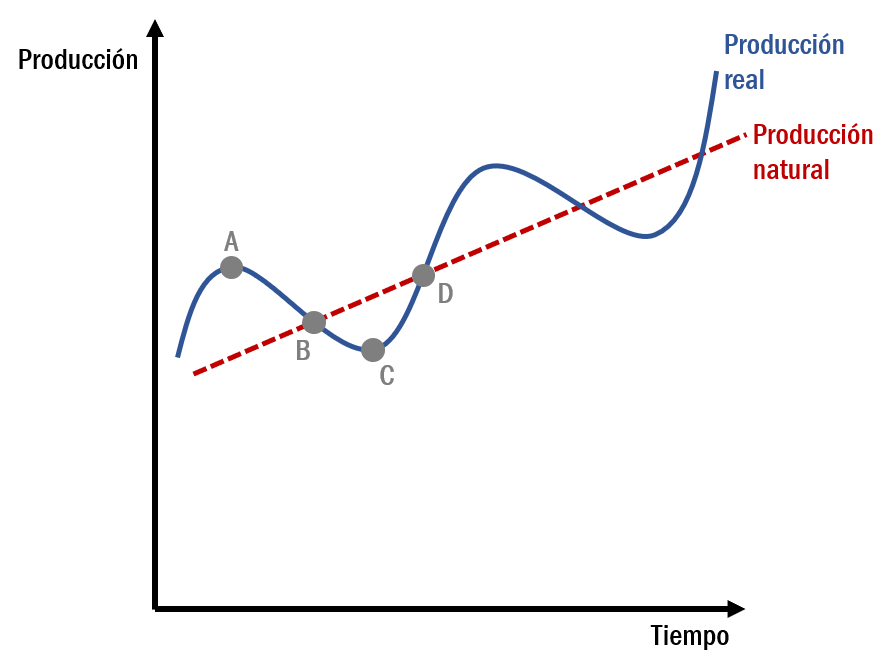
\includegraphics{images/16a-01.png}
\caption{\label{fig:16a-01}Crecimiento a lo largo del tiempo. Oscilaciones y tendencia}
\end{figure}

La tendencia creciente, alrededor de la que fluctúa la produción, se denomina la producción natural o de equilibrio a largo plazo. ¿Cómo se determina la producción natural? En primer lugar, está determinada por la cantidad de recursos productivos y por la tecnología de la que dispone la sociedad. Sin embargo, no puede definirse como el máximo que puede producirse con estos recursos ya que, en este nivel de producción natural existe un cierto porcentaje de recursos que están desempleados. En este aspecto, el concepto de producción natural es diferente del concepto de frontera de posibilidades de producción que estudiamos anteriormente.

Este porcentaje de recursos desempleados que se verifica en la producción natural se denomina la tasa natural de desempleo o tasa de desempleo de equilibrio. Esta tasa natural sería aquella alrededor de la cual oscila la tasa de desempleo. ¿Por qué en la producción natural existe desempleo? Porque los mercados de factores productivos, y en especial el mercado de trabajo, se caracterizan por la existencia de rigideces y comportamientos no competitivos que tienden a convertir el desempleo en algo permanente. ¿Por qué la producción agregada tiende a volver a la producción natural aunque muchas veces se aparte de ésta? Porque el mercado de a esta tasa natural de desempleo.

La evolución sugerida por la Figura \ref{fig:16a-01} sugiere dos preguntas a las que la macroeconomía debe responder: a) ¿por qué la producción natural es creciente?, b) ¿por qué la producción agregada real oscila alrededor de la producción natural y tiende a volver a ella? Las dos preguntas se responden por separado, dando lugar a dos teorías distintas, ya que estudian dos aspectos diferentes de la macroeconomía.

\begin{enumerate}
\def\labelenumi{\alph{enumi})}
\item
  ¿Por qué la tendencia o producción natural es creciente? Si tomamos un período bastante largo de tiempo en que nos permita obviar las oscilaciones (ya que las desviaciones por encima se pueden compensar con las oscilaciones por debajo), observamos que la producción agregada tiene una tendencia creciente. La producción crece con el tiempo porque aumentan las disponibilidades de recursos productivos y mejora la tecnología. El estudio del aumento de la producción natural de un país se lleva a cabo a través de ecimiento económico, que constituye un enfoque a muy largo plazo.
\item
  ¿Por qué la producción oscila alrededor de la tendencia y tiende a volver a ella? La producción oscila, ya que la utilización de factores productivos no siempre se mantiene estable y, por tanto, la tasa de desempleo de estos recursos irá cambiando con el tiempo. La tasa de desempleo oscila alrededor de la tasa natural de desempleo. La producción agregada va oscilando describiendo períodos de crisis y períodos de expansión. En la fase de crisis, la producción cae por debajo de la producción natural, la utilización de recursos es baja y la tasa de desempleo es superior a la natural (punto C de la Figura \ref{fig:16a-01}. Por el contrario, en la fase de expansión la producción supera a la natural, la utilización de recursos es alta y la tasa de desempleo es inferior a la tasa natural de desempleo (punto A de la Figura \ref{fig:16a-01}). Por último, podemos encontrar situaciones en las que la utilización de recursos es tal que la producción agregada se iguala a la producción natural y la tasa de desempleo coincide con la tasa natural de desempleo (puntos B y D de la Figura \ref{fig:16a-01}). Del estudio de las oscilaciones de la producción alrededor de la producción natural se ocupa la teoría del ciclo económico, que analiza los motivos por los que la producción se aparta de su nivel natural a corto plazo, pero tiende a regresar a este nivel a largo plazo. Para estudiar las desviaciones de la producción natural y el regreso a ésta, se considerará que las dotaciones de recursos y la tecnología se mantienen constantes. Por tanto, estudiar el ciclo se considerará que la producción natural es constante.
\end{enumerate}

\begin{quote}
La producción crece en el muy largo plazo porque mejora la tecnología y aumentan las dotaciones de recursos. La teoría del crecimiento económico estudia esta tendencia en el muy largo plazo.
\end{quote}

\begin{quote}
Las oscilaciones de la producción (ciclos) se deben a que cambia la utilización de los recursos productivos disponibles: se reduce en las crisis y aumenta en las fases de expansión. En las crisis la tasa de desempleo es superior a la tasa natural de desempleo, mientras que en las fases deexpansión la tasa de desempleo es inferior a este valor. La teoría del ciclo económico estudia los motivos por los que la producción agregada se separa de su nivel natural a corto plazo pero tiende a regresar a él a largo plazo.
\end{quote}

\hypertarget{la-productividad}{%
\section{La productividad}\label{la-productividad}}

El estudio de la productividad y del crecimiento económico comenzarán desarrollando un modelo muy sencillo basado vagamente en Robinson Crusoe, la novela de Daniel Defoe, acerca de un marino que naufragó en una isla desierta. Puesto que Crusoe vive solo, pesca sus peces, cultiva sus vegetales y confecciona su ropa. Podemos pensar que tales actividades de Crusoe son una economía simple. Al analizar la economía de Crusoe podemos aprender algunas lecciones que también se aplican a economías más complejas y realistas.

¿Qué determina la calidad de vida de Robinson Crusoe? En una palabra, la productividad; es decir, la cantidad producida de bienes y servicios por cada unidad del insumo trabajo. Si Crusoe es bueno pescando, cultivando vegetales y produciendo ropa, vivirá muy bien. Si no es bueno realizando estas tareas vivirá mal. Puesto que Crusoe sólo consume lo que produce, entonces su calidad de vida está vinculada a su productividad.

En el caso de la economía de Crusoe, es fácil notar que la productividad es el determinante clave de la calidad de vida, y que incrementar la productividad es el determinante clave del incremento de la calidad de vida. Mientras más peces atrape por hora, podrá comer más en la cena. Si encuentra un mejor lugar para pescar, aumenta su productividad. Este incremento de la productividad hace que Crusoe se encuentre en mejor situación: puede comer pescado extra o pasar menos tiempo pescando y dedicar más a elaborar otros bienes de los que disfruta.

El rol clave de la productividad para determinar la calidad de vida es tan cierto para las naciones como para los marinos que naufragan en una isla desierta. Debemos recordar que el producto interno bruto (PIB) de una economía mide dos aspectos a la vez: el ingreso total ganado por todos en la economía y la producción de bienes y servicios de la economía. El PIB puede medir de forma simultánea estos dos aspectos, porque para la economía como un todo deben ser iguales. Dicho de una manera sencilla, el ingreso de una economía es la producción de la economía.

Al igual que Crusoe, una nación puede disfrutar de una alta calidad de vida sólo si puede producir una gran cantidad de bienes y servicios. Los estadounidenses viven mejor que los nigerianos porque producen más. Los japoneses han disfrutado de un crecimiento económico más rápido que los argentinos debido a que han experimentado un incremento más rápido de la productividad. De hecho, uno de los diez principios de la economía en es que el estándar o calidad de vida de un país depende de su capacidad para producir bienes y servicios.

Por consiguiente, para comprender las grandes diferencias en la calidad de vida que observamos en los distintos países a lo largo del tiempo, debemos enfocarnos en la producción de bienes y servicios. Pero ver el vínculo entre calidad de vida y productividad es sólo el primer paso y conduce naturalmente a la siguiente pregunta: ¿por qué algunas economías son mucho mejores que otras en la producción de bienes y servicios?

Aun cuando la productividad es importante en un aspecto único para determinar el estándar o calidad de vida de Robinson Crusoe, muchos factores determinan su productividad. Por ejemplo, él sería mejor atrapando peces si tuviera más cañas de pescar, si lo hubieran capacitado en las mejores técnicas de pesca, si su isla tuviera un suministro más abundante de peces o si inventara una carnada mejor. Cada uno de estos determinantes de la productividad de Crusoe, que podemos llamar capital físico, capital humano, recursos naturales y conocimiento tecnológico, tiene una contraparte en las economías más complejas y realistas. Consideremos cada uno de los factores a la vez.

\textbf{Capital físico por trabajador.} Los trabajadores son más productivos si cuentan con las herramientas adecuadas para trabajar. El conjunto de equipo y estructuras que se usa para producir bienes y servicios se denomina capital físico, o simplemente capital. Por ejemplo, cuando los carpinteros fabrican muebles usan sierras, tornos y prensas. Una mayor cantidad de herramientas permitirá que los carpinteros fabriquen más muebles con mayor rapidez y precisión: un trabajador con las herramientas manuales básicas puede fabricar cada semana menos muebles que un trabajador que tenga un equipo sofisticado y especializado para trabajar la madera.

Recuerde que los insumos que se usan para producir bienes y servicios, trabajo, capital, etcétera, se llaman factores de la producción. Una característica importante del capital es que es un factor producido de la producción. Es decir, el capital es un insumo para el proceso de producción que en el pasado fue un producto o resultado del proceso de producción. El carpintero usa un torno para elaborar las patas de la mesa. Antes, el torno mismo fue la producción de una empresa que lo fabricó. El fabricante de tornos, a su vez, usó otro equipo para fabricar su producto. Por consiguiente, el capital es un factor de la producción que se utiliza para producir toda clase de bienes y servicios, inclusive más capital.

\textbf{Capital humano por trabajador.} Un segundo determinante de la productividad es el capital humano. que es el término que emplean los economistas para el conocimiento y las habilidades que adquieren los trabajadores por medio de la educación, la capacitación y la experiencia. El capital humano incluye las habilidades acumuladas en los programas de educación preescolar, la escuela elemental o primaria, la de segunda enseñanza o secundaria, el bachillerato, la universidad y la capacitación laboral para los adultos en la fuerza laboral o población económicamente activa.

La educación, la capacitación y la experiencia son menos tangibles que los tornos, los tractores niveladores y los edificios, pero el capital humano es en muchas formas como el capital físico. Lo mismo que el capital físico, el capital humano incrementa la capacidad de una nación para producir bienes y servicios. Además, lo mismo que el capital físico, el capital humano es un factor producido de la producción. La producción de capital humano requiere insumos en forma de profesores, bibliotecas y tiempo del estudiante. De hecho, se podría considerar a los estudiantes como ``trabajadores'' que tienen la labor importante de generar el capital humano que se utilizará en la producción futura.

\textbf{Recursos naturales por trabajador.}. Un tercer determinante de la productividad es el de los recursos naturales. Los recursos naturales son los insumos de producción que proporciona la naturaleza, como tierra, ríos y depósitos minerales. Los recursos naturales asumen dos formas: renovables y no renovables. Un bosque es un ejemplo de recurso renovable, ya que cuando se tala un árbol, es posible sembrar una planta de vivero en su lugar para que produzca en el futuro. El petróleo es un ejemplo de un recurso no renovable. Puesto que la naturaleza ha producido el petróleo durante varios millones de años, sólo hay un suministro limitado. Una vez que se agote, será imposible crear más.

Las diferencias en los recursos naturales son responsables de algunas de las diferencias en los estándares o calidad de vida de todo el mundo. El éxito histórico de Estados Unidos se debió, en parte, a las grandes extensiones adecuadas de tierras para la agricultura. Hoy, algunos países en Medio Oriente, como Kuwait y Arabia Saudita, son ricos simplemente porque sucede que se encuentran situados encima de los pozos petroleros más grandes del mundo.

Aun cuando los recursos naturales pueden ser importantes, no son necesarios para que una economía sea altamente productiva en la generación de bienes y servicios. Por ejemplo, Japón es uno de los países más ricos del mundo, a pesar de contar con pocos recursos naturales. El comercio internacional hace que su éxito sea posible, ya que este país importa muchos recursos naturales que necesita, como petróleo, y exporta bienes manufacturados a las economías ricas en recursos naturales.

\textbf{Conocimiento tecnológico.} Un cuarto determinante de la productividad es el conocimiento tecnológico; es decir, la comprensión de la mejor forma de producir bienes y servicios. Hace 100 años la mayoría de los estadounidenses trabajaba en granjas, debido a que éstas necesitaban gran cantidad del insumo trabajo para alimentar a toda la población. Hoy, gracias a los avances tecnológicos en la agricultura, una pequeña fracción de la población puede producir suficientes alimentos para satisfacer a todo el país. Este cambio tecnológico hizo que la mano de obra estuviera disponible para producir otros bienes y servicios.

El conocimiento tecnológico adopta muchas formas. Parte de la tecnología es del conocimiento común: después de que una persona la utiliza, todos son conscientes de ella. Por ejemplo, una vez que Henry Ford introdujo con éxito la producción en líneas de montaje, otros fabricantes de automóviles lo imitaron rápidamente. Otra tecnología es protegida o patentada, ya que sólo la conoce la empresa que la inventa. Por ejemplo, sólo Coca-Cola Company conoce la fórmula secreta para producir su famosa bebida refrescante. Y, por su parte, otras tecnologías están patentadas a corto plazo. Cuando una compañía farmacéutica descubre un nuevo medicamento, el sistema de patentes le otorga a esa empresa un derecho temporal de ser su fabricante exclusivo. Sin embargo, cuando expira la patente, otras empresas son autorizadas para producir el medicamento. Todas estas formas de conocimiento tecnológico son importantes para que la economía produzca bienes y servicios.

Vale la pena distinguir entre conocimiento tecnológico y capital humano. Aun cuando están estrechamente relacionados, existe una diferencia importante. El conocimiento tecnológico se refiere a la comprensión de la sociedad acerca de cómo funciona el mundo. El capital humano se refiere a los recursos que se gastan para transmitirle esta comprensión a la fuerza laboral. Para utilizar una metáfora pertinente, el conocimiento es la calidad de los libros de texto de la sociedad, mientras que el capital humano es la cantidad de tiempo que la población ha dedicado a leerlos. La productividad de los trabajadores depende de ambos.

\hypertarget{lograr-crecimiento-econuxf3nico}{%
\section{Lograr crecimiento econónico}\label{lograr-crecimiento-econuxf3nico}}

Hasta ahora se ha determinado que el estándar o calidad de vida de una sociedad depende de su capacidad para producir bienes y servicios y que, a su vez, su productividad depende del capital físico, del capital humano, de los recursos naturales y del conocimiento tecnológico, todos por cada trabajador. Ahora volvamos a la pregunta que enfrentan quienes diseñan las políticas en todo el mundo: ¿qué puede hacer una política gubernamental para incrementar la productividad y la calidad de vida?

\hypertarget{ahorro-e-inversiuxf3n}{%
\subsection{Ahorro e inversión}\label{ahorro-e-inversiuxf3n}}

Dado que el capital es un factor producido de la producción, una sociedad puede modificar la cantidad de capital que tiene. Si hoy una economía produce una gran cantidad de nuevos bienes de capital, entonces mañana tendrá una mayor existencia de capital y podrá producir más bienes y servicios. Por consiguiente, la única manera de incrementar la productividad futura es invertir más recursos actuales en la producción de capital.

Uno de los Diez principios de la economía es que las personas enfrentan disyuntivas. Este principio es especialmente importante cuando consideramos la acumulación de capital. Puesto que los recursos son escasos, si se dedican más al capital, eso requiere dedicar menos a la producción de bienes y servicios para el consumo actual. Es decir, para que la sociedad invierta más en capital, debe consumir menos y ahorrar más de su ingreso actual. El crecimiento que se origina de la acumulación de capital no es gratuito: requiere que la sociedad sacrifique el consumo de bienes y servicios en el presente con la finalidad de disfrutar de un mayor consumo en el futuro.

En el siguiente capítulo se estudia con más detalle la forma en la cual los mercados financieros de la economía coordinan el ahorro y la inversión. También se analiza la forma en la cual las políticas gubernamentales influyen en la cantidad de ahorro e inversión que tiene lugar. En este punto es importante observar que alentar el ahorro y la inversión es una forma en la que un gobierno puede estimular el crecimiento y, en el largo plazo, mejorar la calidad de vida de la economía.

\hypertarget{rendimientos-decrecientes-y-efecto-de-convergencia}{%
\subsection{Rendimientos decrecientes y efecto de convergencia}\label{rendimientos-decrecientes-y-efecto-de-convergencia}}

Suponga que un gobierno sigue políticas que incrementan la tasa de ahorro del país, es decir, el porcentaje del pib que se dedica al ahorro y no al consumo. ¿Qué sucede? Si la nación ahorra más, se necesitan menos recursos para fabricar bienes de consumo y se dispone de más recursos para fabricar bienes de capital. Como resultado, las existencias de capital se incrementan, lo que conduce a un incremento de la productividad y a un crecimiento más rápido del pib. ¿Pero cuánto dura esta tasa más alta de crecimiento? Suponga que la tasa de ahorro se mantiene en su nuevo nivel más alto, ¿la tasa de crecimiento del pib se mantiene indefinidamente alta o sólo durante un periodo?

El punto de vista tradicional del proceso de producción es que el capital está sujeto a rendimientos decrecientes: a medida que aumentan las existencias de capital, disminuye la producción extra producida por una unidad adicional de capital. En otras palabras, cuando los
trabajadores ya tienen una gran cantidad de capital para producir bienes y servicios, si se les da un incremento de una unidad adicional de capital, eso incrementa sólo ligeramente la productividad. Esto se ilustra en la figura 1, que muestra la forma en la cual la cantidad de capital determina la cantidad de producción por trabajador, manteniendo constantes todos los demás determinantes de la producción.

Debido a los rendimientos decrecientes, un incremento de la tasa de ahorro conduce a un mayor crecimiento sólo durante algún tiempo. A medida que la mayor tasa de ahorro permite una mayor acumulación de capital, los beneficios de una unidad adicional de capital disminuyen a lo largo del tiempo y el crecimiento también disminuye. En el largo plazo, la tasa más alta de ahorro conduce a un nivel más alto de productividad e ingreso, pero no a un mayor crecimiento de esas variables. Sin embargo, llegar a ese largo plazo podría llevar mucho tiempo. Según los estudios de datos internacionales sobre el crecimiento económico, el incremento de la tasa de ahorro puede conducir a un crecimiento considerable durante un periodo de varias décadas.

Los rendimientos decrecientes para el capital tienen otra implicación importante: si todo lo demás permanece igual, es más fácil para un país crecer con mayor rapidez si comienza siendo relativamente pobre. A este efecto de las condiciones iniciales sobre el crecimiento subsiguiente en ocasiones se le llama efecto de convergencia. En los países pobres, los trabajadores carecen incluso de las herramientas más rudimentarias y, como resultado, tienen una productividad baja. Los pequeños montos de inversión en capital incrementarían de forma significativa la productividad de esos trabajadores. Por el contrario, los trabajadores de países ricos tienen grandes cantidades de capital para trabajar, y esto explica en parte su productividad más alta. Sin embargo, con la cantidad de capital por trabajador ya tan alta, una inversión adicional de capital tiene un efecto relativamente pequeño sobre la productividad. Los estudios con datos internacionales sobre el crecimiento económico confirman este efecto de convergencia: al controlar otras variables, como el porcentaje del pib dedicado a la inversión, los países pobres tienden a crecer más rápidamente que los ricos.

Este efecto de convergencia puede explicar algunos otros hechos enigmáticos. He aquí un ejemplo: de 1960 a 1990 Estados Unidos y Corea del Sur dedicaron una parte similar del pib a la inversión. Sin embargo, a lo largo de ese tiempo, Estados Unidos sólo experimentó un crecimiento mediocre de alrededor de 2\% anual, mientras que Corea del Sur experimentó un crecimiento espectacular de más de 6\%. La explicación es el efecto de convergencia. En 1960 Corea del Sur tenía un pib por persona menor de una décima parte del nivel de Estados Unidos, en parte debido a que la inversión previa había sido muy baja. Con un pequeño capital inicial, los beneficios de la acumulación de capital fueron mucho mayores en Corea del Sur, y eso le dio a ese país una mayor tasa de crecimiento.

Este efecto de convergencia también aparece en otros aspectos de la vida. Cuando una escuela le otorga un premio al final del año al estudiante ``que más mejoró'', ese estudiante por lo general es uno que inició el año con un desempeño relativamente deficiente. Los estudiantes que iniciaron el año no estudiando encuentran que mejorar es más fácil que los estudiantes que siempre trabajaron arduamente. Debemos observar que es bueno ser el ``que más mejoró'' dado el punto de partida, pero es todavía mejor ser el ``mejor estudiante''. De manera similar, el crecimiento económico a lo largo de las últimas décadas ha sido mucho más rápido en Corea del Sur que en Estados Unidos, pero el pib por persona es todavía más alto en Estados Unidos.

\hypertarget{inversiuxf3n-extranjera}{%
\subsection{Inversión extranjera}\label{inversiuxf3n-extranjera}}

Hasta ahora hemos analizado la forma en la cual las políticas orientadas a incrementar la tasa de ahorro de un país pueden incrementar la inversión y, por consiguiente, el crecimiento económico a largo plazo. El ahorro de los residentes domésticos o nacionales no es la única forma de que un país invierta en capital nuevo. La otra forma es la inversión que realizan los extranjeros.

La inversión extranjera asume varias formas. Ford Motor Company podría construir una planta en México. Una inversión de capital que es propiedad y está operada por una entidad extranjera se llama inversión extranjera directa. Asimismo, un estadounidense podría comprar acciones de una empresa o corporación mexicana (es decir, adquirir una parte de la propiedad de la empresa); la empresa mexicana puede emplear los ingresos para construir una nueva planta. Una inversión financiada con dinero del extranjero, pero operada por residentes nacionales, se denomina inversión extranjera de cartera. En ambos casos, los estadounidenses proporcionan los recursos necesarios para incrementar las existencias de capital en México. Es decir, el ahorro de los estadounidenses se utiliza para financiar la inversión mexicana.

Cuando los extranjeros invierten en un país, lo hacen porque esperan que dicha inversión genere un rendimiento sobre su inversión. La planta de Ford incrementa las existencias de capital en México y, por consiguiente, la productividad y el PIB mexicanos. Sin embargo, Ford se lleva parte de ese ingreso adicional a Estados Unidos en forma de utilidades. De manera similar, cuando un inversionista estadounidense compra acciones mexicanas, el inversionista tiene derecho a una participación de la utilidad que gana la corporación mexicana.

Por consiguiente, la inversión extranjera no tiene el mismo efecto sobre todas las medidas de la prosperidad económica. Debemos recordar que el producto interno bruto (PIB) es el ingreso ganado dentro de un país, tanto por los residentes como por los no residentes, mientras que el producto nacional bruto (PNB) es el ingreso ganado por los residentes de un país tanto dentro del mismo como en el extranjero. Cuando Ford abre su planta automotriz en México, parte del ingreso que genera la planta se acumula para personas que no viven en ese país. Como resultado, la inversión extranjera en México incrementa el ingreso de los mexicanos (medido por el PNB), menos de lo que aumenta la producción de México (medida por el PIB).

Sin embargo, la inversión extranjera es una vía para que crezca un país. Aun cuando algunos de los beneficios de esta inversión fluyen de regreso a los inversionistas extranjeros, esta inversión sí incrementa las acciones de capital de la economía, lo que conduce a mayor productividad y salarios más altos. Además, la inversión extranjera es una forma para que los países pobres aprendan las tecnologías más modernas que se desarrollan y usan en países más ricos. Por estas razones, numerosos economistas que asesoran a los gobiernos en países menos desarrollados recomiendan políticas que alientan la inversión extranjera. A menudo, esto significa eliminar las restricciones que han impuesto los gobiernos sobre la propiedad extranjera del capital nacional.

Una organización que trata de fomentar el flujo de capital hacia los países pobres es el Banco Mundial. Esta organización internacional obtiene fondos de los países avanzados del mundo, como Estados Unidos, y los utiliza para hacer préstamos a los países menos desarrollados, con la finalidad de que puedan invertir en carreteras, alcantarillado, escuelas y otros tipos de capital. También les ofrece a los países asesoría sobre cómo se podrían utilizar mejor los fondos. El Banco Mundial, junto con su organización hermana, el Fondo Monetario Internacional, se fundaron después de la Segunda Guerra Mundial. Una lección de la guerra fue que la zozobra económica a menudo conduce a disturbios políticos, tensiones internacionales y conflictos militares. Por consiguiente, todos los países tienen interés en promover la prosperidad económica en el mundo. El Banco Mundial y el Fondo Monetario Internacional se establecieron para lograr esa meta común.

\hypertarget{educaciuxf3n}{%
\subsection{Educación}\label{educaciuxf3n}}

La educación, que es la inversión en capital humano, es al menos tan importante como la inversión en capital físico para el éxito económico de un país en el largo plazo. En Estados Unidos, cada año de escolaridad ha incrementado históricamente el salario de una persona un promedio de alrededor de 10\%. En los países menos desarrollados, en donde el capital humano es especialmente escaso, la brecha entre los salarios en la cual la política gubernamental puede mejorar la calidad de vida es proporcionar buenas escuelas y alentar a la población para que las aproveche.

La inversión en capital humano, lo mismo que en capital físico, tiene un costo de oportunidad. Cuando los estudiantes se dedican a la escuela, se privan de los salarios que podrían haber ganado como miembros de la fuerza laboral o población económicamente activa. En los países menos desarrollados, los niños a menudo abandonan la escuela a una edad temprana, aun cuando el beneficio de la escolaridad es muy alto, simplemente porque se necesita su trabajo para ayudar a sostener a la familia.

Algunos economistas han argumentado que el capital humano es particularmente importante para el crecimiento económico, debido a que transmite externalidades positivas. Una externalidad es el efecto de las acciones de una persona en el bienestar de otros. Por ejemplo, una persona preparada podría generar nuevas ideas acerca de cómo producir de mejor forma los bienes y servicios. Si esas ideas forman parte del conjunto de conocimientos de una sociedad, de manera que todos las puedan utilizar, entonces las ideas son un beneficio externo de la educación. En este caso, el rendimiento de la escolaridad para la sociedad es todavía mayor que el rendimiento para la persona. Este argumento justificaría los grandes subsidios para la inversión en capital humano que se observan en la forma de educación pública.

Un problema que enfrentan algunos países pobres es la fuga de talentos o cerebros, es decir, la migración de muchos de los trabajadores más preparados a los países ricos, en donde pueden disfrutar de mayor calidad de vida. Si el capital humano tiene externalidades positivas, entonces esta fuga hace que las personas que permanecen en el país de origen sean más pobres de lo que serían de otra manera. Este problema les presenta un dilema a quienes diseñan las políticas. Por una parte, Estados Unidos y otros países ricos tienen los mejores sistemas de educación superior, y parecería natural que los países pobres enviaran al extranjero a sus mejores estudiantes para obtener posgrados. Por otra parte, esos estudiantes que han pasado algún tiempo en el extranjero podrían decidir no volver a su país de origen, y este tipo de fuga de talentos reduciría aún más el capital humano del país pobre.

\hypertarget{salud-y-nutriciuxf3n}{%
\subsection{Salud y nutrición}\label{salud-y-nutriciuxf3n}}

El término capital humano se refiere por lo general a la educación, pero también se puede utilizar para describir otro tipo de inversión en las personas: gastos que conducen a tener una población más saludable. Si todo lo demás permanece igual, los trabajadores más saludables son más productivos. Las inversiones en la salud de la población proporcionan una forma para que país incremente su productividad y mejore su calidad de vida.

El historiador económico Robert Fogel ha sugerido que un factor significativo del crecimiento económico en el largo plazo es una mejor salud debida a una mejor nutrición. Estima que en Gran Bretaña, en 1780, alrededor de una de cada cinco personas estaba tan desnutrida que no podía realizar trabajos manuales. Entre aquellos que podían trabajar, la ingestión insuficiente de calorías reducía de forma significativa el esfuerzo laboral que podían realizar. A medida que mejoraba la alimentación, también lo hacía la productividad de los trabajadores.

Fogel estudia estas tendencias históricas enfocándose en la estatura de la población. La estatura baja puede ser un indicador de mala nutrición, en especial durante los periodos de gestación y los primeros años de vida. Fogel encuentra que a medida que las naciones se desarrollan económicamente, las personas comen más y la población es más alta. De 1775 a 1975, la ingesta promedio de calorías consumidas en Gran Bretaña aumentó 26\% y la estatura del hombre promedio aumentó 3.6 pulgadas. De manera similar, durante el espectacular crecimiento económico de Corea del Sur de 1962 a 1995, el consumo de calorías aumentó 44\% y la estatura del hombre promedio aumentó aproximadamente 2 pulgadas. Por supuesto, la estatura es determinada por una combinación de predisposición genética y del ambiente. Pero debido a que la constitución genética de la población cambia lentamente, es más probable que esos incrementos en la estatura promedio se deban a cambios en el ambiente, y la nutrición es la explicación más clara.

Además, algunos estudios han revelado que la estatura es un indicador de la productividad. Al ver los datos de muchos trabajadores en cierto punto en el tiempo, los investigadores han encontrado que los de mayor estatura tienden a ganar más. Puesto que los salarios reflejan la productividad de un trabajador, este descubrimiento sugiere que los trabajadores de mayor estatura tienden a ser más productivos. El efecto de la estatura en los salarios es especialmente pronunciado en los países más pobres, en donde la desnutrición es un riesgo mayor.

Fogel ganó el Premio Nobel de Economía en 1993 por su trabajo en historia económica, que no sólo incluye sus estudios de nutrición, sino también de la esclavitud en Estados Unidos y el papel de los ferrocarriles en el desarrollo de la economía estadounidense. En la conferencia que impartió cuando ganó el premio acerca de la evidencia sobre la salud y el crecimiento económico, concluyó que ``las mejoras en la nutrición explican aproximadamente 30\% del incremento del ingreso per cápita en Gran Bretaña entre 1790 y 1980''.

Por fortuna, hoy la desnutrición es rara en los países desarrollados como Gran Bretaña y Estados Unidos. (La obesidad es un problema más gave.) Pero para las personas en los países en desarrollo, la mala salud y la nutrición inadecuada siguen siendo obstáculos para una mayor productividad y mejorar la calidad de vida. La Organización de las Naciones Unidas estima que casi un tercio de la población en África subsahariana está desnutrida.

El vínculo causal entre la salud y la riqueza corre en ambas direcciones. Los países pobres lo son en parte porque sus poblaciones no disfrutan de buena salud, y sus poblaciones no disfrutan de buena salud en parte porque son pobres y no se pueden permitir una atención médica y una nutrición adecuadas. Es un círculo vicioso. Sin embargo, este hecho abre la posibilidad de un círculo virtuoso: las políticas que conducen a un crecimiento económico más rápido, naturalmente mejorarían la salud, lo que a su vez promoverá el crecimiento económico.

\hypertarget{derechos-de-propiedad-y-estabilidad-poluxedtica}{%
\subsection{Derechos de propiedad y estabilidad política}\label{derechos-de-propiedad-y-estabilidad-poluxedtica}}

Otra forma en la cual quienes diseñan las políticas pueden fomentar el crecimiento económico es protegiendo los derechos de propiedad y promoviendo la estabilidad económica. Este aspecto llega al fondo mismo de la forma en la cual operan las economías de mercado.

La producción en las economías de mercado se origina de las interacciones de millones de personas y empresas. Por ejemplo, cuando usted compra un automóvil, está adquiriendo la producción de un distribuidor automotriz, un fabricante de automóviles, una compañía acerera, una empresa de mineral de hierro, etc. Esta división de la producción entre muchas empresas permite que los factores de producción de la economía se utilicen en forma tan eficiente como sea posible. Para alcanzar este resultado, la economía debe coordinar las transacciones entre esas empresas, así como entre las empresas y los consumidores. Las economías de mercado logran esta coordinación por medio de los precios de mercado. Es decir, dichos precios son los instrumentos mediante los cuales la mano invisible del mercado equilibra la oferta y la demanda en cada uno de los muchos miles de mercados que conforman la economía.

Un requisito previo importante para que funcione el sistema de precios es el respeto de los derechos de propiedad en toda la economía. Tales derechos se refieren a la capacidad de las personas para ejercer autoridad sobre los recursos que poseen. Una empresa minera no hará el esfuerzo para extraer mineral de hierro si espera que le roben éste. La al sólo si confía en que se beneficiará con su venta subsiguiente.

Por esta razón, los tribunales desempeñan un rol muy importante en la economía de mercado: exigen que se respeten los derechos de propiedad. Por medio del sistema de justicia penal, los tribunales desalientan el robo directo. Además, mediante el sistema de justicia civil, los tribunales se aseguran de que compradores y vendedores cumplan sus contratos.

Aquellos que viven en países desarrollados tienden a dar por sentados los derechos de propiedad, pero quienes viven en países menos desarrollados comprenden que la carencia de derechos de propiedad puede ser un problema importante. En muchos países el sistema de justicia no funciona bien. Es difícil exigir el cumplimiento de los contratos, y los fraudes por lo general quedan impunes. En casos más extremos, el gobierno no sólo fracasa para hacer valer los derechos de propiedad, sino que en realidad los infringe. Para hacer negocios en algunos países, se espera que las empresas sobornen a los funcionarios del gobierno. Esta corrupción dificulta el poder de coordinación de los mercados y desalienta el ahorro interno y la inversión extranjera.

Una amenaza a los derechos de propiedad es la inestabilidad política. Cuando las revoluciones y las revueltas son comunes, existe la duda acerca de si los derechos de propiedad se respetarán en el futuro. Si un gobierno revolucionario pudiera confiscar el capital de algunas empresas, como ha sucedido a menudo después de las revoluciones comunistas, los residentes nacionales tendrán menos incentivos para ahorrar, invertir y abrir nuevas empresas. Al mismo tiempo, los extranjeros tienen menos incentivos para invertir en el país. Incluso la sola amenaza de una revolución puede actuar para afectar la calidad de vida de una nación.

Por consiguiente, la prosperidad económica depende en parte de la prosperidad política. Un país con un sistema judicial eficiente, con funcionarios públicos honestos y una constitución estable disfrutará de un mayor estándar económico de vida que un país con un sistema judicial deficiente, funcionarios deshonestos y frecuentes revoluciones y golpes de estado.

\hypertarget{libre-comercio}{%
\subsection{Libre comercio}\label{libre-comercio}}

Algunos de los países más pobres del mundo han tratado de lograr un crecimiento económico más rápido buscando políticas orientadas al interior. Estas políticas tratan de incrementar la productividad y la calidad de vida dentro del país, evitando la interacción con el resto del mundo. Las empresas nacionales o domésticas a menudo expresan el argumento de la industria incipiente, afirmando que necesitan protección de la competencia extranjera para prosperar y crecer. Junto con una desconfianza de los extranjeros, este argumento ha conducido a quienes diseñan las políticas en países menos desarrollados a aplicar aranceles y otras restricciones comerciales.

Hoy, la mayoría de los economistas cree que los países pobres estarían mejor si buscaran políticas orientadas al exterior e integraran a esos países en la economía mundial. El comercio internacional de bienes y servicios puede mejorar el bienestar económico de los ciudadanos de un país. En ciertas formas, el comercio es un tipo de tecnología. Cuando un país exporta trigo e importa textiles, se beneficia como si hubiera inventado una nueva tecnología para convertir el trigo en textiles. Por consiguiente, un país que elimina las restricciones comerciales experimentará la misma clase de crecimiento económico que ocurriría después de un avance tecnológico importante.

El impacto adverso de la orientación hacia el interior se vuelve claro cuando se considera el pequeño tamaño de muchas economías menos desarrolladas. Por ejemplo, el pib total de Argentina es similar al de Houston, Texas. Imagine lo que sucedería si el consejo municipal de Houston les prohibiera a los residentes comerciar con personas que viven fuera de los límites de la ciudad. Sin poder aprovechar las ganancias del comercio, Houston necesitaría producir todos los bienes que consume. También tendría que producir todos sus bienes de capital, en vez de importar un equipo moderno de otras ciudades. La calidad de vida en Houston disminuiría de inmediato y quizás el problema se agudizaría con el transcurso del tiempo. Esto es precisamente lo que sucedió cuando Argentina siguió políticas orientadas al interior durante gran parte del siglo xx. En contraste, los países que siguieron políticas orientadas al exterior, como Corea del Sur, Singapur y Taiwán, han disfrutado de altas tasas de crecimiento económico.

El volumen que un país comercia con otros es determinada no sólo por las políticas del gobierno, sino también por la geografía. A los países que tienen puertos marítimos naturales les resulta más fácil comerciar que a los que carecen de este recurso. No es coincidencia que muchas de las principales ciudades del mundo, como Nueva York, San Francisco y Hong Kong, estén ubicadas cerca de los océanos, junto al mar. De manera similar, debido a que los países que no tienen salida al mar encuentran que el comercio internacional es más difícil, tienden a tener menores niveles de ingreso que los países con un fácil acceso a los canales de navegación del mundo. Por ejemplo, los países con más de 80\% de su población que vive a menos de 100 kilómetros de la costa tienen un pib promedio alrededor de cuatro veces mayor que los que tienen menos de 20\% de su población que vive cerca de una costa. La importancia crucial del acceso al mar ayuda a explicar por qué el continente africano, que tiene muchos países rodeados de tierra, es tan pobre.

\hypertarget{investigaciuxf3n-y-desarrollo}{%
\subsection{Investigación y desarrollo}\label{investigaciuxf3n-y-desarrollo}}

La razón principal de que la calidad de vida sea más alta en la actualidad que hace un crecimiento tecnológico. El teléfono, el transistor, la computadora y el motor de combustión interna se encuentran entre las miles de innovaciones que han mejorado la capacidad para producir bienes y servicios.

La mayoría de los avances tecnológicos proviene de la investigación privada de empresas e inventores individuales, pero también hay un interés público en promover tales esfuerzos. En general, el conocimiento es un bien público; es decir, una vez que una persona descubre una idea, ésta pasa a formar parte del conjunto de conocimientos de la sociedad y otras personas la pueden utilizar libremente. Así como el gobierno desempeña un rol al proveer un bien público, como la defensa nacional, también desempeña uno para fomentar la investigación y el desarrollo de nuevas tecnologías.

Desde hace largo tiempo, el gobierno estadounidense, ha desempeñado un rol en la creación y propagación del conocimiento tecnológico. Hace un siglo, el gobierno patrocinaba la investigación acerca de métodos agrícolas y asesoraba a los granjeros sobre la mejor forma de utilizar sus tierras. Más recientemente, el gobierno estadounidense, a través de la NASA y de la Fuerza Aérea, ha apoyado la investigación aeroespacial; como resultado, Estados Unidos es un fabricante importante de cohetes y aviones. El gobierno sigue fomentando los avances en el conocimiento con subvenciones de investigación de la Fundación Nacional para la Ciencia y los Institutos Nacionales de Salud, y también con deducciones de impuestos para las empresas dedicadas a la investigación y el desarrollo.

Otra forma en la cual la política del gobierno fomenta la investigación es el sistema de patentes. Cuando una persona o una empresa inventan un producto, como un nuevo medicamento, el inventor puede solicitar una patente. Si se considera que el producto es verdaderamente original, entonces el gobierno se la otorga, lo que le concede al inventor el derecho exclusivo de fabricarlo durante un número específico de años. En esencia, la patente le confiere al inventor un derecho de propiedad sobre su invención, convirtiendo su nueva idea de un bien público en un bien privado. Al permitir que los inventores obtengan utilidades de sus invenciones, aun cuando sólo sea de manera temporal, el sistema de patentes mejora el incentivo para que las personas y las empresas se dediquen a la investigación.

\hypertarget{crecimiento-de-la-poblaciuxf3n}{%
\subsection{Crecimiento de la población}\label{crecimiento-de-la-poblaciuxf3n}}

Los economistas y otros científicos sociales desde hace largo tiempo han debatido la forma en la cual la población afecta a la sociedad. El efecto más directo es en el tamaño de la fuerza laboral: una población grande significa más trabajadores para producir bienes y servicios. El tremendo tamaño de su población es una razón por la cual China es un actor tan importante en la economía mundial.

Sin embargo, al mismo tiempo una población grande significa que hay más personas para consumir esos bienes y servicios. De manera que, aun cuando una población más grande significa una mayor producción total de bienes y servicios, eso no significa necesariamente mayor calidad de vida para un ciudadano típico. De hecho, países grandes y pequeños se encuentran en todos los niveles de desarrollo económico.

\hypertarget{la-poluxedtica-econuxf3mica}{%
\chapter{La política económica}\label{la-poluxedtica-econuxf3mica}}

\hypertarget{objetivos-de-la-poluxedtica-econuxf3mica}{%
\section{Objetivos de la política económica}\label{objetivos-de-la-poluxedtica-econuxf3mica}}

Desde una perspectiva macroeconómica, los gobiernos buscan la consecución de cuatro grandes objetivos:

\begin{itemize}
\tightlist
\item
  Conseguir crecimiento económico. Esto significa ampliar la capacidad Productiva del país para elaborar bienes y servicios. El crecimiento económico se mide en la tasa a la que crece el PIB real.
\item
  Controlar la inflación. Este objetivo busca controlar la tasa de crecimiento de los precios (IPC) para defender el poder adquisitivo de los salarios nominales, de modo de mantener el bienestar de la población.
\item
  Reducir el desempleo. Se trata de lograr pleno empleo de los recursos productivos, especialmente de la mano de obra. Pleno empleo no significa 0\% de desempleo, sino que implica aceptar una cierta tasa de desempleo natural.
\item
  Equilibrio externo o equilibrio en balanza de pagos. El proceso de apertura y globalización de las economías, hace necesario velar por mantener cuentas externas sanas, con saldos moderados y controlables por las autoridades económicas.
\end{itemize}

Para lograr estos objetivos, las autoridades económicas cuentan con variados instrumentos de política económica. Estos instrumentos permiten determinar el ritmo y rumbo de la actividad económica. Según la bibliografía común, existen dos grandes políticas (la fiscal y la monetaria) y otras que, aunque relevantes, suelen tener un menor peso relativo que las dos anteriores (la política comercial exterior y la política de oferta). Vamos a presentar los elementos que caracterizan a cada una de ellas.

\hypertarget{la-poluxedtica-fiscal}{%
\section{La política fiscal}\label{la-poluxedtica-fiscal}}

Las políticas fiscales son políticas económicas de demanda a través de las cuales el gobierno actúa sobre sus ingresos y gastos para influenciar los niveles de ingresos, producción, y desempleo de la economía. El gobierno puede hacer esto vía impuestos sobre la renta y ayudas al desempleo, o con medidas discrecionales, como los impuestos sobre el gasto y aumentando el gasto público. Aumentando la demanda, las empresas son incentivadas a producir más y por tanto a aumentar la contratación de trabajadores.

El keynesianismo creía que las políticas fiscales son la mejor herramienta para controlar la economía de un país, especialmente para reducir el desempleo cíclico. El monetarismo y otras doctrinas como la nueva macroeconomía clásica y la nueva economía keynesiana consideran estas medidas ineficaces a largo plazo, ya que la demanda no puede aumentar continuamente.

La política fiscal se refiere a las decisiones que determinan los presupuestos generales del Estado, e implican la utilización del gasto público, los impuestos y las transferencias para influir sobre la demanda total de la economía y, así, incidir significativamente sobre el nivel de la producción y renta.

El gasto público incluye las compras del Estado en bienes y servicios, como por ejemplo, la construcción de carreteras, el pago a funcionarios, la compra de ferrocarriles, de aviones, de armamento, etc. Las transferencias del Estado son todos los pagos realizados por el gobierno a familias y empresas que no se corresponden a ninguna actividad productiva, como por ejemplo, las pensiones, las prestaciones de desempleo, las ayudas familiares, etc. Por último, los impuestos son los ingresos corrientes del Estado que proceden de los contribuyentes.

La política fiscal, a través de sus instrumentos, condiciona el consumo y el ahorro privado, y a partir de estas variables, influyen en la producción y en la inversión, primero a corto plazo y más tarde a largo plazo. Por otra parte, la política fiscal incide sobre los precios de los bienes y de los factores de producción y, por tanto, afectan a los incentivos y a la conducta de los individuos.

Una política fiscal expansiva consiste en elevar el gasto total de la economía a través del aumento de las compras del Estado, el aumento de las transferencias o las bajadas de los impuestos sobre la renta. Una política fiscal restrictiva o contractiva es lo contrario: disminución de las compras del Estado, disminución de las transferencias o aumento de los impuestos.

\hypertarget{la-poluxedtica-moneraria}{%
\section{La política moneraria}\label{la-poluxedtica-moneraria}}

Las políticas monetarias son políticas económicas de demanda a través de las cuales el banco central de un país actúa sobre la cantidad de dinero y los tipos de interés para influenciar los niveles de ingresos, producción y desempleo en la economía, siendo el tipo de interés el nexo entre dinero e ingreso. Las principales herramientas usadas por la política monetaria son las operaciones de mercado abierto, los préstamos a los bancos y la modificación de los requisitos de reservas mínimas. Ceteris paribus, un aumento (disminución) en la oferta monetaria o una disminución (aumento) en los tipos de interés tendrá un efecto positivo (negativo) sobre el gasto privado (consumo e inversión). Esto aumentará (disminuirá) finalmente la producción y el empleo. Sin embargo, esto provocará un aumento de los precios, que puede dar lugar a una rápida y creciente inflación.

El monetarismo es la principal doctrina económica que defendía estas políticas. El keynesianismo, la nueva macroeconomía clásica y la nueva economía keynesiana critican estas medidas y no creen en su efectividad ya que ha sido demostrado que un aumento de la oferta monetaria traerá una inflación que contrarrestará los efectos positivos. Como Milton Friedman decía, ``la inflación es siempre y en todo lugar un fenómeno monetario''.

En el ámbito del Unión Europea, la política monetaria la realiza el Banco Central Europeo (BCE) y su objetivo principal es tratar de mantener estables los precios. Para ello, el Banco Central Europeo controla la evolución de la cantidad de dinero u oferta monetaria dentro de la Unión Europea (los billetes y monedas es el dinero legal, pero el mayor componente del dinero en las economías modernas es el que se crea dentro del propio sistema bancario a partir de los préstamos, y que sólo figura como apunte bancario). A partir de este control monetario se determinará la cantidad disponible de crédito bancario y, en general, se regulará el funcionamiento del sistema financiero.

Mediante el control de la oferta monetaria el BCE fijará los tipos de interés de referencia en la economía y, con ello, incidirá en la inversión, en el consumo, en la producción, en el nivel general de precios, en los tipos de cambio (y, consiguientemente, en las exportaciones y en las importaciones), en los precios de las acciones y en el precio de las viviendas. De este modo, la política monetaria trata de evitar, o al menos paliar, los inconvenientes derivados de los ciclos económicos.

Un aumento de la cantidad de dinero, con la consiguiente disminución del tipo de interés, es una política monetaria expansiva. Una disminución de la cantidad de dinero con su correspondiente aumento del tipo de interés es una política monetaria restrictiva.

\hypertarget{la-poluxedtica-de-oferta}{%
\section{La política de oferta}\label{la-poluxedtica-de-oferta}}

El objetivo de las políticas económicas de oferta es aumentar la cantidad ofertada y por tanto el potencial productivo que una economía posee. Este tipo de políticas mueve hacia la derecha la curva de oferta agregada a largo plazo y hacia el exterior la frontera de posibilidades de producción. Pueden ser divididas en políticas que actúan sobre la función de producción y aquellas que actúan sobre los costes laborales.

Las primeras están dirigidas a aumentar los niveles de producción siendo un ejemplo las políticas que incluyen incentivos al progreso tecnológico y el aumento de stock de capital. Por otro lado, las últimas se dirigen directamente a disminuir los costes laborales y de este modo más trabajadores pueden ser contratados. Ejemplos de estas políticas son la reducción de la contribución a la seguridad social, el aumento de subsidios empresariales, la reducción de impuestos indirectos, etc.

Las políticas de oferta han sido defendidas por numerosos economistas incluyendo el premio Nobel Robert Mundell. Ha habido numerosos estudios concernientes a su efectividad, y aunque es cierto que tienen efecto a largo plazo, son las únicas que pueden llevar a un crecimiento económico prolongado. Por otro lado, las corrientes monetarista y keynesiana han sido cuestionadas ya que tanto la política monetaria como la fiscal son únicamente usadas en el corto plazo, siendo inútiles e incluso perjudiciales para la economía en el largo plazo. De hecho, las últimas dos grandes doctrinas, la nueva macroeconomía clásica y la nueva economía keynesiana han demostrado la ineficiencia de las políticas monetarias y fiscales, dejando las políticas de oferta como las únicas verdaderamente eficaces para la economía.

La política de oferta puede aplicarse también como un control sobre las rentas. En este caso, consiste en una política, en principio, de consenso o de pacto entre los grandes grupos sociales de la economía (a saber, Estado, sindicatos como representantes de los trabajadores y empresarios) para moderar las subidas de precios y salarios, y con ello frenar las tensiones inflacionistas y/o los aumentos en la tasa de desempleo. Se pretende controlar la evolución de las rentas de la economía para asegurar y mantener una mayor estabilidad tanto de precios como de empleo. El objetivo de la política de rentas es doble. Por un lado, se intenta fomentar la eficiencia económica mediante la reasignación de los recursos. Y por otro, promover la equidad al redistribuir la renta entre los diferentes agentes económicos.

Cuando el Estado no consigue llegar a este tipo de acuerdos entre los agentes implicados, adoptará una política de rentas de ``ordeno y mando'', limitando el precio de determinados productos, congelando o reduciendo los salarios de los funcionarios, estableciendo unos márgenes máximos de subidas de salarios, subvencionando a determinados sectores, o aplicando desgravaciones fiscales, por ejemplo.

\hypertarget{la-poluxedtica-exterior}{%
\section{La política exterior}\label{la-poluxedtica-exterior}}

La política comercial trata de influir directamente en la cantidad de bienes y servicios que importa o exporta un país, con el fin de mejorar el saldo comercial con el exterior (es decir, la diferencia entre las exportaciones y las importaciones). Esta política se instrumentaliza a través de los aranceles (impuestos que gravan con una determinada proporción el precio de un bien importado), contingentes (límites físicos o cuantitativos a la cantidad que se puede importar de un determinado bien) y otros mecanismos (subvenciones o ayudas a la exportación, firma de tratados comerciales ventajosos, libre comercio, etc). Otra práctica utilizada por algunos gobiernos es fijar o determinar unilateralmente los tipos de cambio, esto es, estableciendo el precio de la moneda nacional en relación con las monedas extranjeras.

La política comercial intenta propiciar la eficiencia del comercio internacional mediante una mayor competitividad en el exterior, lo cual favorecerá el crecimiento económico, mayores rentas interiores y una mejora del bienestar.

Consideramos la política exterior como aquella parte de la política general formada por el conjunto de decisiones y actuaciones mediante las cuales se definen los objetivos y se utilizan los medios de un Estado para generar, modificar o suspender sus relaciones con otros actores de la sociedad internacional.

A partir de esta definición de la política exterior, podemos señalar sus principales elementos. En primer término su carácter estatal. En efecto, aunque en sentido metafórico se puede hablar de la política exterior de otros actores internacionales (Movimientos Populares; Organizaciones Gubernamentales; etc.),lo cierto es que la política exterior sólo puede predicarse de los Estados ya que son los únicos actores que reúnen los dos requisitos necesarios para poder desarrollarla plenamente: capacidad jurídica reconocida internacionalmente y capacidad política plena, autónoma y eficaz.

En segundo lugar, la política exterior no puede disociarse de la política interior del Estado. Ambas se interfieren mutuamente ya que, en último extremo, ambas no son mas que dos facetas de una misma realidad política, la del Estado, tanto en su dimensión institucional como en su base social. La diferencia entre estas dos esferas de la política del Estado responde, en último extremo, a la diversidad de formas y órganos que participan en la elaboración de una y otra, así como a sus diferentes destinatarios Mientras la política interior se dirige a los individuos y grupos de una misma sociedad estatal, la política exterior está orientada a permitir la vinculación entre Estados.

Además, como toda política, la exterior se articula por una combinación de decisiones y actuaciones de los órganos estatales, de modo principal por parte del Gobierno, sin solución de continuidad. Cuando se quiebra esta ordenada secuencia entre decisiones y actuaciones, podemos afirmar que el Estado carece de una auténtica política exterior. Entonces podemos hablar de que política exterior y acción exterior se confunden al faltar una capacidad decisional autónoma y verdaderamente política.

Por último, la política exterior incluye la determinación de los fines u objetivos que aspira a alcanzar cada Estado, pero debe también incorporar la especificación y utilización de los medios más adecuados para el logro de esos objetivos. Si el país carece de una determinación de sus fines u objetivos, el Estado simplemente actuará en el contexto internacional reaccionando a los acontecimientos coyunturales, sin que pueda hablarse de una política exterior. Análogamente,si carece de los medios necesarios o son manifiestamente insuficientes para alcanzar los fines que se ha trazado, el Estado evidenciará una escasa proyección internacional fruto,en parte,de la impotencia para dar respuesta a los retos que el contexto internacional o las aspiraciones internas le plantean y,de otra,a la débil credibilidad que su política exterior suscitará entre los demás países.

\hypertarget{el-entorno-econuxf3mico-de-la-empresa}{%
\chapter{El entorno económico de la empresa}\label{el-entorno-econuxf3mico-de-la-empresa}}

La empresa, en el desempeño de su actividad, interactúa constantemente con el entorno que la rodea, ya sea en el mercado de factores productivos, con trabajadores, proveedores y acreedores, así como en el mercado de productos y servicios finales, fundamentalmente con clientes y competidores. Además, la empresa, como el resto de instituciones, organizaciones y personas físicas, se encuentra dentro de un sistema económico, social, cultural, político o legal que condiciona su comportamiento.

Por todo ello, resulta fundamental definir y comprender el funcionamiento del entorno que rodea a la empresa con el objetivo de aprovechar las oportunidades que éste plantea, así como evitar o neutralizar sus amenazas. En sentido amplio, el entorno de la empresa se define como todas aquellas características ajenas a la empresa que ésta no puede controlar, pero que influyen o pueden influir en su actividad, comportamiento y resultados, presentes y futuros.

\begin{figure}
\centering
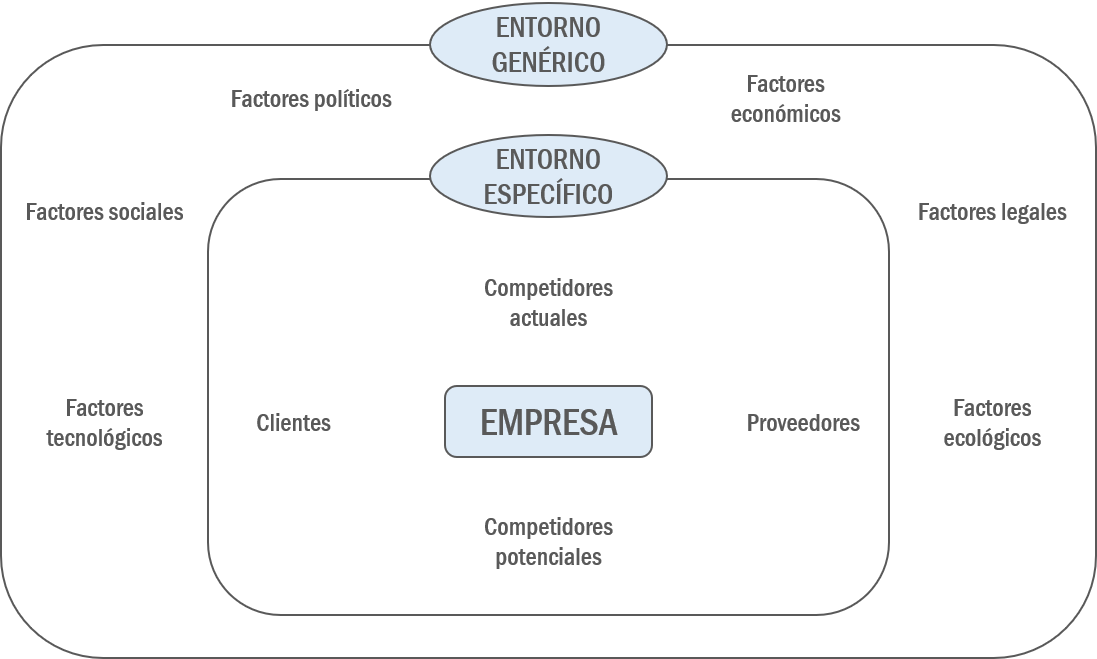
\includegraphics{images/18a-01.png}
\caption{\label{fig:18a-01}El entorno económico de la empresa}
\end{figure}

Con el objetivo estudiar con más detalle el entorno empresarial se diferencian dos niveles de entorno: el entorno general y el entorno específico. El entorno general abarca los factores socioeconómicos, mientras que el entorno específico se identifica con factores relativos al sector donde la empresa compite. En la Figura \ref{fig:18a-01} se proponen los principales aspectos incluidos en estos dos niveles del entorno empresarial.

\hypertarget{el-entorno-genuxe9rico}{%
\section{El entorno genérico}\label{el-entorno-genuxe9rico}}

El entorno general de la empresa se define como el conjunto de variables y factores que desde diferentes ámbitos -económico, político, legal, cultural, social, ecológico, etc.- afecta o puede afectar a todos los agentes económicos y sociales, y por ende, a las empresas, de una determinada sociedad, país o área geográfica determinada.

Para llevar a cabo el análisis del entorno general resulta ampliamente utilizado el denominado análisis PESTEL \citep{johnson2007} que incluye factores del entorno general agrupados bajo las dimensiones Política, Económica, Social, Tecnológica, Ecológica y Legal. Cada uno de ellos debe aplicarse al ámbito geográfico de las actividades de la empresa.

\begin{itemize}
\tightlist
\item
  La dimensión política incluye las variables que configuran el sistema institucional de un determinado país o área geográfica con capacidad política decisoria. Estas variables delimitan las relaciones jurídicas, sociales y económicas entre los diferentes agentes económicos y sociales. Aspectos como el sistema político existente (democrático u otro), la independencia y desarrollo del sistemajudicial, la estabilidad institucional del Estado, el nivel de intervencionismo de las Administraciones Públicas, o la estabilidad del gobierno, son aspectos importantes a considerar por parte de las empresas.
\item
  La dimensión económica engloba aquellas variables macroeconómicas que configuran la situación económica actual y futura de una determinada área geográfica. Entre las variables más representativas, encontramos datos de crecimiento del producto interior bruto (PIB), tasa de desempleo, tipos de interés, tasa de inflación o datos sobre consumo privado, entre otras.
\item
  La dimensión social incluye variables de carácter social, cultural y demográfico. La tasa de natalidad, esperanza de vida, inmigración, nivel educativo de la población, estilos de vida o la aparición de nuevos valores aceptados por la sociedad, son algunos ejemplos de variables incluidas por las empresas para valorar esta dimensión.
\item
  La dimensión tecnológica básicamente se mide por la existencia de infraestructura y desarrollo tecnológico existente, presupuesto público y/o privado dedicado a actividades de investigación, desarrollo e innovación (1+D+i).
\item
  La dimensión ecológica del entorno se refiere al nivel de sensibilización de una sociedad, sus organizaciones políticas, gubernamentales o sociales hacia el medioambiente. Los alimentos transgénicos, la producción contaminante, el consumo energético sostenible o el reciclado de residuos y envases son aspectos que se manifiestan cada vez con mayor ímpetu en diferentes aspectos de una sociedad, que se deberán atender y tener en cuenta por parte de la actividad y comportamiento de la empresa.
\item
  La dimensión legal se refiere a la definición del marco laboral, comercial, financiero o de defensa de la competencia. Está íntimamente ligada a la dimensión política. En este sentido, las leyes para el libre comercio de la Unión Europa o Nafta van más allá de las variables políticas de cada país concreto.
\end{itemize}

Cada empresa deberá seleccionar aquellas variables, dentro de cada dimensión, que sean más relevantes para su actividad empresarial. A partir de la información y datos disponibles, la dirección identificará posibles amenazas a evitar y oportunidades a tener en cuenta en sus actuaciones empresariales. Cabe destacar en este sentido, que una variable puede resultar una amenaza para un determinado sector de actividad y puede constituirse en una oportunidad para otro y no ser relevante para un tercer sector de actividad, e incluso, que dentro de una misma industria, suponga una amenaza para la mayoría de empresas competidoras, pero para una o unas pocas constituya una oportunidad.

\hypertarget{el-entorno-especuxedfico}{%
\section{El entorno específico}\label{el-entorno-especuxedfico}}

El análisis del entorno específico o competitivo de la empresa complementa el estudio de los factores externos que influyen o pueden influir en la actividad de la empresa y en sus resultados. El análisis del entorno específico tiene su origen en los estudiosos de la Economía Industrial \citep{bain1958}, los cuales proponen que la estructura de la industria donde opera la empresa condiciona el comportamiento estratégico de ésta y sus competidoras, y por ende, los resultados a obtener.

Lo relevante en el análisis del entorno específico es determinar el grado de atractivo de la industria. Dicho atractivo indicará la probabilidad que la empresa tiene de obtener rentas o beneficios en dicho sector, lo que vendrá determinado por las oportunidades y amenazas que el sector depare para las empresas que están ubicadas en él. Así, una industria será más atractiva cuantos mayores sean los factores que representan oportunidades para las empresas allí instaladas y menores sean los factores que representan amenazas. En caso contrario, hablaremos de industrias poco atractivas.

\hypertarget{herramientas-para-el-anuxe1lisis-del-entorno-de-la-empresa}{%
\section{Herramientas para el análisis del entorno de la empresa}\label{herramientas-para-el-anuxe1lisis-del-entorno-de-la-empresa}}

La técnica o herramienta más empleada para el análisis de la estructura de la industria y su grado de atractivo es el conocido Modelo de las Cinco Fuerzas Competitivas o Modelo de Porter (\citet{porter1982}) (Figura \ref{fig:18a-02}).

\begin{figure}
\centering
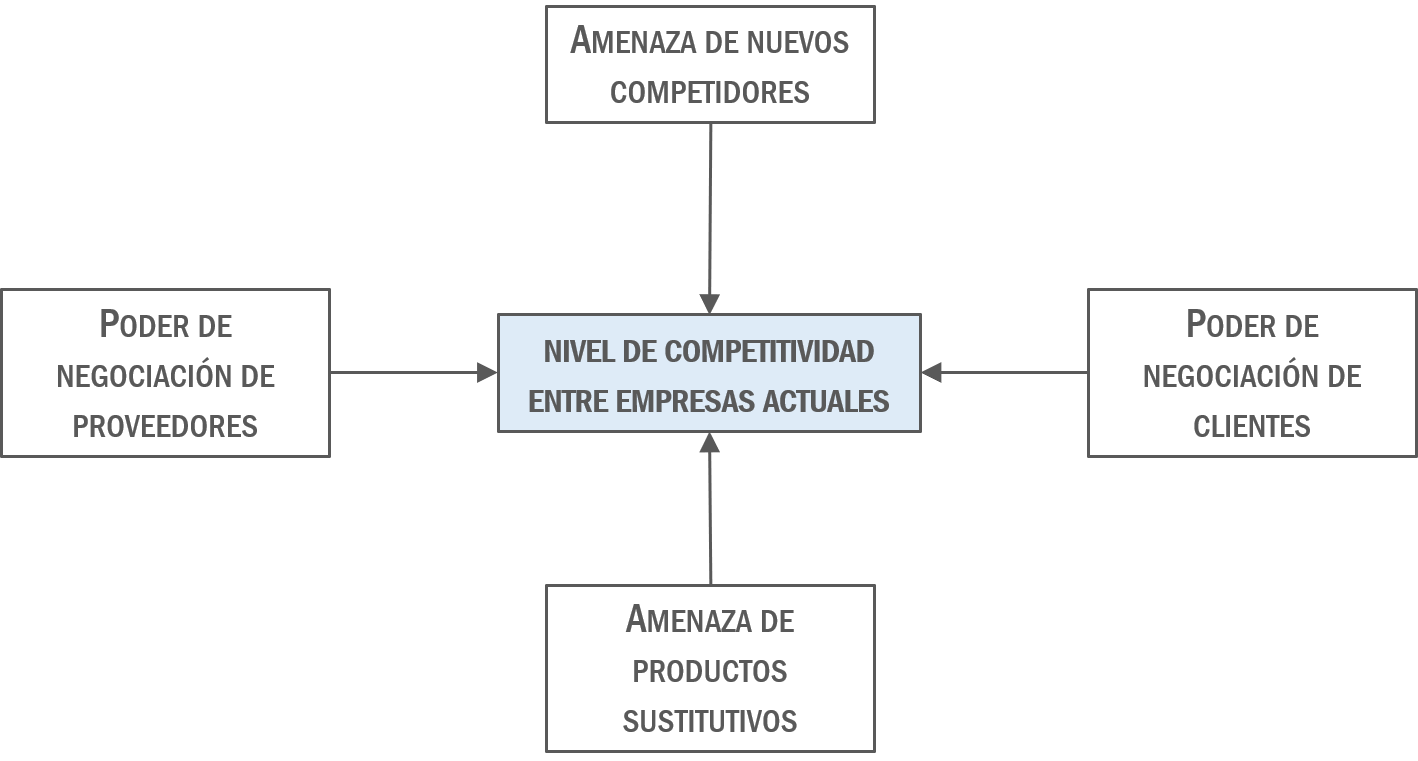
\includegraphics{images/18a-02.png}
\caption{\label{fig:18a-02}Modelo de las cinco fuerzas de Porter}
\end{figure}

\hypertarget{el-anuxe1lisis-de-porter}{%
\subsection{El análisis de Porter}\label{el-anuxe1lisis-de-porter}}

De acuerdo con este modelo el grado de atractivo de la industria depende de las siguientes cinco fuerzas competitivas:

\textbf{Grado de rivalidad de la competencia actual}

Esta fuerza está formada por el conjunto de empresas que son rivales y que, por tanto, compiten con la empresa en la venta de sus productos. Cuanto mayor sea el grado de rivalidad entre los competidores actuales de una determinada industria, menor será su grado de atractivo. Entre los factores que inciden en dicho grado de rivalidad, destacamos los siguientes:

\begin{itemize}
\tightlist
\item
  Número de competidores. Cuanto mayor sea el número de empresas competidoras existentes en una industria y más compensado esté su tamaño relativo, mayores incentivos existen a la confrontación directa para ganar cuota de mercado, y por tanto, mayor resultará el grado de rivalidad de la competencia actual.
\item
  Crecimiento de la demanda. En industrias donde la demanda está estancada, las empresas se ven forzadas a una mayor rivalidad, tratando de conseguir clientes de la competencia para aumentar sus ventas. Por el contrario, cuando la demanda agregada de una industria crece mucho, la rivalidad se reduce porque las empresas incrementan sus ventas directamente de los nuevos clientes que van apareciendo o por la mayor demanda de los existentes.
\item
  Grado de diferenciación. Cuando los productos que los diferentes competidores ofrecen son homogéneos o estandarizados la competencia es más dura y se suele centrar en ofrecer un precio atractivo. No obstante, cuando los productos de la industria se pueden diferenciar a través de distintas prestaciones, marca, servicios, garantías, calidad, etc., cada empresa puede centrarse en un tipo de producto y la competencia se atenúa.
\item
  Tamaño mínimo eficiente elevado. Cuando en la industria es importante tener un gran tamaño para empezar a competir y ofrecer productos a precios competitivos, las empresas tienen que realizar un elevado volumen de inversiones y con objeto de recuperarlas lanzan al mercado gran cantidad de los productos, incidiendo de esta manera en un aumento en el grado de rivalidad de la competencia actual.
\item
  Existencia de barreras de salida. Las barreas de salida se refieren a la imposibilidad real que pueden llegar a tener las empresas para cesar sus actividades y abandonar el mismo. Suele ocurrir en negocios que no tienen futuro en el sector, y las barreras de salida pueden ser instalaciones específicas que impiden su adecuada venta o reutilización, factores emocionales que impiden el abandono, tener que despedir a muchas personas, etc. En la medida en que existan barreras de salida y éstas impidan de manera efectiva la salida «natural» de las empresas peor dotadas, el grado de rivalidad de los competidores actuales de una industria aumentará.
\end{itemize}

\textbf{Amenaza de entrada de nuevos competidores}

Además de conocer el grado de rivalidad de las empresas competidoras actuales de una industria, resulta conveniente analizar la amenaza de entrada de nuevas empresas competidoras, que en caso de producirse, vendrían a aumentar dicha rivalidad, deteriorando el grado de atractivo de la industria. Esta amenaza viene determinada fundamentalmente por:

\begin{itemize}
\tightlist
\item
  Existencia de barreras de entrada. Se refiere a la existencia de obstáculos, como la necesidad de tener una marca consolidada, un gran volumen de producción, licencias administrativas, etc., que impiden la entrada libre a nuevos competidores a un determinado sector de actividad o industria. Pueden entenderse como desventajas que las empresas que quieren entrar tienen frente a las ya establecidas. Desventajas que, al margen de factores políticos, pueden subsanarse pero implican tiempo e inversión económica para las empresas. Cuantas mayores sean estas barreras de entrada, más dilicil será la entrada de nuevos rivales en la industria.
\item
  Reacción de las empresas competidoras ya instaladas. Este factor puede tener un resultado similar a la existencia de las barreras de entrada, en tanto exista una fuerte y dura reacción de las empresas ya instaladas en el sector hacia los nuevos entrantes. Estas reacciones pueden ser aumentar la gama de productos, reducir los márgenes sobre ventas iniciando «una guerra de precios», establecer negociaciones en exclusiva con sus distribuidores, aumentar los servicios complementarios, etc.
\end{itemize}

\textbf{Amenaza de productos sustitutivos}

Los productos sustitutivos son productos que satisfacen las mismas necesidades que los de la empresa, si bien utilizan otra tecnología, es decir, suelen provenir de otro sector. Por ejemplo, un producto sustitutivo de los viajes en avión puede ser el tren. Sin duda, el grado en que un producto es más o menos sustitutivo depende de los clientes, de cómo lo valoren y del precio que cada uno tiene. Ahora bien, cuanto más amenaza exista de la aparición de productos sustitutivos, menos atractivo será el sector.

Esta fuerza estará limitada por la existencia de costes de cambio por parte de los clientes, es decir, de lo fácil o barato que resulte a éstos cambiar del producto actual al producto sustitutivo. Así por ejemplo, el cambio de una compañía de teléfono a otra se vio durante un tiempo limitado porque los usuarios perdían su número de teléfono. Cuantos mayores sean los costes de cambio, menor será la amenaza de productos sustitutivos.

\textbf{Poder de negociación de clientes}

Esta fuerza hace referencia al grado en el cual los clientes de una determinada industria tienen poder relativo para negociar precios y demás aspectos relevantes del proceso de compra, imponiendo unas condiciones de intercambio favorables a ellos. En este sentido, cuanto mayor sea su poder de negociación, menor será el grado de atractivo de la industria. Entre los factores que condicionan dicho poder de negociación, se encuentran los siguientes:

\begin{itemize}
\tightlist
\item
  Grado de concentración e importancia de los clientes en relación con la industria. Cuando los clientes de la industria son muy pocos, estando concentradas las ventas de la industria en unos pocos clientes, las empresas de la industria tienen pocas alternativas para vender sus productos, por lo que el poder negociador se reduce en beneficio de sus clientes.
\item
  Grado de diferenciación de los productos objeto de la transacción. Cuando en la industria se ofrecen productos altamente valorados por los clientes debido a sus características únicas, los clientes tendrán una mayor dependencia hacia la industria y su poder de negociación se reducirá.
\item
  Otros aspectos importantes son el grado de información sobre la transacción que tengan los clientes, influyendo positivamente en su poder de negociación frente a las empresas de la industria, así como la amenaza real de integración hacia atrás (posibilidad real de que un cliente se convierta en su propio proveedor y por lo tanto no necesite de las empresas de la industria).
\end{itemize}

\textbf{Poder de negociación de proveedores}

Los factores que explican el poder negociador de los proveedores frente a las empresas de la industria son, en esencia, similares a los comentados en relación con el poder de negociación de los clientes, pero en sentido contrario. Así, el poder negociador de proveedores hace referencia al grado en el cual pueden negociar precios y demás aspectos relevantes del proceso de venta, imponiendo unas condiciones de intercambio favorables a ellos. En este sentido, cuanto mayor sea el poder de negociación de los proveedores, menor será el grado de atractivo de la industria. Entre los factores que condicionan dicho poder de negociación, se encuentran los siguientes:

\begin{itemize}
\tightlist
\item
  Grado de concentración e importancia de los proveedores en relación con la industria. Cuando los proveedores de la industria son muy pocos, estando concentradas las compras de la industria en unos pocos proveedores, las empresas de la industria tienen pocas alternativas para comprar sus materias primas y otros inputs, por lo que el poder negociador se reduce en beneficio de sus proveedores.
\item
  Grado de diferenciación de los productos objeto de la transacción. Cuando los proveedores ofrecen productos altamente valorados por las empresas de la industria debido a sus características únicas, las empresas compradoras tendrán una mayor dependencia hacia los proveedores y su poder de negociación se reducirá.
\item
  Otros aspectos importantes son el grado de información sobre la transacción que tengan los proveedores, influyendo positivamente en su poder de negociación frente a las empresas de la industria, así como la amenaza real de integración hacia delante de los mismos (posibilidad real de que un proveedor se convierta en su propio cliente y por lo tanto no necesite de las empresas de la industria).
\end{itemize}

\hypertarget{el-anuxe1lisis-dafo}{%
\subsection{El análisis DAFO}\label{el-anuxe1lisis-dafo}}

Texto.

\hypertarget{part-la-administraciuxf3n-de-empresas}{%
\part{La Administración de Empresas}\label{part-la-administraciuxf3n-de-empresas}}

\hypertarget{la-direcciuxf3n-de-empresas}{%
\chapter{La dirección de empresas}\label{la-direcciuxf3n-de-empresas}}

La dirección es un área fundamental para el correcto funcionamiento de toda organización que tenga un objetivo. No es necesaria por tanto sólo en las empresas, sino en todo tipo de organización, del tipo que ésta sea, aunque por razones obvias en estos apuntes nos centraremos en el caso de las empresas.

En una empresa se reúnen recursos de características muy diferentes y es función de la dirección, el conseguir que trabajen de forma común para conseguir los objetivos que se planteen. La dirección debe encargarse de asignar y coordinar los recursos existentes, así como estimular su mejora continua y fomentar la generación de nuevos recursos. Este aumento de recursos no se refiere únicamente a los tangibles, generados en forma de inversiones, sino también a los intangibles como es la mejora del conocimiento de los empleados, de sus habilidades, o la consolidación de la imagen de la marca de la empresa en el mercado.

Desde un punto de vista más científico, se plantea la dirección de una empresa como un proceso en el que se realizan varias funciones. Las más clásicas son la planificación, la organización, la dirección de recursos humanos y el control.

Planificar consiste en decidir por adelantado qué vamos a querer hacer en el futuro y con qué medios vamos a dotarnos para realizarlo. Supone tomar una serie de decisiones de forma anticipada pero nos permite determinar qué queremos conseguir, cómo vamos a lograrlo y qué recursos vamos a comprometer en la tarea. Sin embargo, la planificación se debe entender como una ayuda, no como una limitación inamovible. No debe ser un fin mismo, sino una manera de reducir la incertidumbre del futuro.

Organizar se refiere al diseño de la estructura organizativa de la empresa, o lo que es lo mismo, las relaciones entre todos sus miembros. La jerarquía, frente a la opinión de que toda autoridad es mala, es un sistema eficiente de asignación de recursos y surge de la especialización y división del trabajo. La organización jerárquica de una empresa se plasma de una forma sencilla en su organigrama, y en él se reflejan los distintos niveles y puestos organizativos en los que se divide la empresa.

La dirección de recursos humanos integra a los individuos dentro de la estructura organizativa anterior, de tal forma que se consiga la correcta adecuación de los mismos para el logro de los objetivos de la empresa. Para conseguir este objetivo, se debe realizar el reclutamiento, selección, entrenamiento y asignación de las personas a cada uno de los puestos de la empresa.

Por último, el control busca comprobar que el funcionamiento de la empresa se desarrolla dentro de la planificación desarrollada. En caso contrario, el control es el encargado de realizar las correcciones necesarias. Es así pues un complemento a la función de planificación, pues es el control es el encargado de garantizar su cumplimiento. El control consiste en general en medir los resultados obtenidos y compararlos con los esperados para a partir de ahí, identificar diferencias y analizar la forma de corregirlas.
Cada una de estas funciones brevemente desarrolladas aquí son las que se van a explicar en los siguientes temas, así que sirva este pequeño apartado como introducción al bloque de la asignatura en el que nos encontramos.

\hypertarget{funciones-directivas}{%
\section{Funciones directivas}\label{funciones-directivas}}

El trabajo de dirección se puede entender como el conjunto de la serie de actividades o funciones específicas que la integran. Los más básicos de estos conceptos son los siguientes:

\begin{enumerate}
\def\labelenumi{\arabic{enumi}.}
\tightlist
\item
  PREDICCIÓN. Proyección o extrapolación de datos o de información actual para estimar el valor futuro de una magnitud económica o el estado del sistema. También se llama pronóstico.
\item
  PREVISIÓN. Conocimiento del valor más probable de una magnitud económica en una fecha futura, a través de la aplicación de un método de análisis de datos.
\item
  ESTRATEGIA. Modelo de decisión que revela la misión y objetivos de la organización, así como los planes y políticas para lograrlos, de forma que defina su posición competitiva respecto en qué negocio está o quiere estar.
\item
  PLANIFICACIÓN. Estudio y fijación de objetivos y metas, tanto referentes al sistema total como a cada subsistema, aspecto, función y unidad organizativa, incluyendo los cursos de acción que los desarrollan a largo y corto plazo.
\item
  POLÍTICA. Respuesta concreta o guía para pensar y decidir respecto de una situación dada o a un problema específico, de forma que permita obtener la solución prevista.
\item
  PROGRAMACIÓN. Análisis operativo a corto y medio plazo para llevar a cabo una adecuada asignación de recursos y la aplicación de los consiguientes sistemas de solución de objetivos planificados.
\item
  PRESUPUESTACIÓN. Cuantificación financiera y adaptación temporal de los planes y programas elaborados, de forma que permita una adecuada asignación de responsabilidades a las unidades de actuación y facilite el control de los objetivos.
\item
  PROCEDIMIENTO. Conjunto de normas, instrucciones y recomendaciones obligatorias que sirven de guía para la acción o para llevar a cabo las actividades que logran los objetivos.
\item
  REGLA. Orden o norma para hacer o no hacer alguna acción, de forma que no permita la discrecionalidad.
\item
  DECISIÓN. Elección lo más racional posible de las alternativas de un curso de acción para lograr la consecución de los objetivos.
\item
  CONTROL. Proceso de observación y medida a través de la comparación sistemática de los objetivos con los resultados obtenidos.
\end{enumerate}

Al mantener relaciones interpersonales, se crea a su alrededor una red de comunicaciones, lo que le permite realizar una serie de labores informativas. Como monitor recoge información, y como difusor y portavoz distribuye información, dentro de la empresa en la primera, fuera en el caso de la segunda función.

Por último, el poseer la información que gestiona en los papeles anteriores, le capacita para tomar decisiones, con lo que cumple con el último bloque de roles, los decisorios. El directivo es empresario, gestor de anomalías, asignador de recursos y negociador.

\hypertarget{la-toma-de-decisiones}{%
\section{La toma de decisiones}\label{la-toma-de-decisiones}}

Una de las características principales de la administración de la empresa es la de convertir la información en acción. Este paso, es lo que se denomina decisión. La decisión sólo puede producirse cuando el decisor se plantea distintas alternativas sobre las que está perfectamente informado y de las que conoce con precisión cuáles serán sus consecuencias.

La toma de decisiones por tanto se define como la elección racional entre alternativas para lograr la consecución de un objetivo, y es algo intrínseco a la tarea directiva de la empresa. Decidir se asemeja mucho a resolver un problema: cuando algo no marcha bien, cuando algo no funciona, es necesario tomar una decisión para resolver el conflicto.

Al igual que no todos los problemas o conflictos son iguales, todas las soluciones no lo son tampoco. Estas diferencias nos permiten distinguir entre decisiones, según el tipo de problema y la solución que se adopta. Así, podemos separar entre decisiones rutinarias (aquellas con problemas conocidos y que nos permiten programar una respuesta para solucionarlos), adaptativas (aquellas que suponen cambios incrementales sobre la situación precedente; procesos de mejora continua) o innovadoras (aquella mal estructurada, única y novedosa que exige un tratamiento especial).

Según otros autores, esta clasificación de las decisiones se puede realizar también con base a otros criterios, como puede ser el nivel directivo (decisión estratégica global, específica u operativa), la función directiva (decisiones de producción, de comercialización, de financiación, etc.), el horizonte temporal (decisión a largo o a corto plazo) o las características del problema de decisión (decisión programada o no programada).

\hypertarget{el-proceso-de-toma-de-decisiuxf3n}{%
\subsection{El proceso de toma de decisión}\label{el-proceso-de-toma-de-decisiuxf3n}}

El proceso decisorio es algo más que la selección de una alternativa entre varias. Es un conjunto de actividades que deben seguirse en un orden lógico y que abarca desde la identificación del problema hasta la puesta en marcha de acciones que tienen como objetivo resolverlo.

El primer paso es como se ha dicho ya la identificación del problema. No debe bastar con una mera identificación, sino que debe profundizarse y analizar las características del mismo, así como sus síntomas y causas.

El siguiente paso a tomar es la búsqueda de las posibles soluciones. De todas las posibles alternativas de solución que se presenten, será necesario realizar una evaluación. Esta evaluación debe estar diseñada de antemano, por lo que antes de proceder al análisis de las posibles soluciones, será necesario fijar los criterios de evaluación que vamos a utilizar para el análisis de las alternativas.

Decidir consiste en optar entre estas alternativas. Para realizarlo de una forma racional, debemos comparar las alternativas, identificando sus consecuencias, lo que puede esperarse de cada una de ellas y a partir de ahí, elegir la mejor de acuerdo con el criterio de evaluación elegido.

Una vez que hemos elegido la mejor alternativa según nuestros criterios, tan sólo queda su puesta en marcha. Este es el último paso y con el que queda cerrado el proceso decisorio. Toda decisión debe transformarse en una acción.

Es importante ver cómo en cada uno de los pasos que conforman la toma de decisiones, la información es vital, es la materia prima del proceso. Gracias a la información, somos capaces de identificar bien un problema y sus características, buscar alternativas, evaluarlas y llegado el momento, proceder a la puesta en práctica de la solución elegida.

\hypertarget{los-niveles-y-roles-directivos}{%
\section{Los niveles y roles directivos}\label{los-niveles-y-roles-directivos}}

Las tareas directivas de una empresa tienen tal cierto grado de complejidad que es común que una única persona no pueda ocuparse de todas ellas. El trabajo directivo, como cualquier otro, va experimentando una relativa especialización de tal forma que van apareciendo nuevos puestos no directamente productivos cuya función es la coordinación del resto de personal de la empresa.

El diseño de la estructura de la empresa consiste en ir coordinando el trabajo que se realiza en cada nivel con la creación de una serie de puestos directivos que a su vez, tendrán un control superior. Esto es lo que conforma la estructura piramidal de la organización. Esta jerarquía surge cuando se pone un equipo de trabajo bajo las órdenes de un capataz, que a su vez se encuentra sometido a las instrucciones un directivo de mayor nivel, que estará subordinado a otro de índole superior y así sucesivamente.

En principio, una división sencilla de los niveles directivos los clasifica en tres grupos, en función de sus tareas y responsabilidades: la alta dirección, los directivos de nivel medio y los supervisores de primera línea.

La alta dirección es la encargada de conducir el rumbo de la empresa, fijando sus objetivos y sus líneas estratégicas, estableciendo la marcha general y haciendo que todo funcione de una forma cohesionada. A este nivel afectan multitud de factores, estando entre ellos los medioambientales, lo que hace que se experimente una cierta incertidumbre y que los problemas que surgen sean nuevos y mal comprendidos. Por todo ello, las decisiones que suelen tomarse en este nivel son poco estructuradas y a largo plazo, basándose más en la prueba-error que en otro método, por lo que la reflexión, el buen juicio y la experiencia son básicos en este nivel.

Los directivos de primera línea son aquellos que se encuentran en contacto directo con los trabajadores productivos de la empresa. Ocupan el nivel más bajo de entre todos los que dan órdenes a otros y a diferencia del nivel anterior, las decisiones que se toman en este nivel suelen ser rutinarias y repetitivas, casi siempre con los mismos problemas, por lo que es posible dedicar los recursos al estudio de estos problemas y a la búsqueda de la solución óptima.

Entre ambos niveles, aparecen los directivos de nivel medio, que son los encargados de realizar las tareas de unión entre ambos niveles. Tanto sus superiores como sus subordinados son directivos y su papel básico consiste en transmitir información: en sentido descendente comunican las grandes líneas empresariales fijadas por el nivel superior en forma de objetivos, planes y programas concretos para cada directivo de primera línea, asignando los recursos necesarios; en sentido ascendente coordinan e integran las tareas de los niveles inferiores.

Cada nivel de los anteriores requiere de diferentes combinaciones de conocimientos y habilidades conceptuales, humanas y tecnológicas, aunque en todos los niveles se necesitará de buenas dosis de destrezas humanas, puesto que en todo trabajo directivo, el trato y la relación con otras personas es algo importante.

\hypertarget{planificaciuxf3n-y-control}{%
\chapter{Planificación y control}\label{planificaciuxf3n-y-control}}

La planificación se centra en la búsqueda de la forma de lograr el futuro deseado para la empresa. Implica determinar la misión de la misma y los objetivos a conseguir, y por tanto, las acciones a realizar para alcanzar ese estado final deseado. Para ello se realizan los planes, tanto a corto como a largo plazo, en los que además de todo lo anterior, se recoge la distribución de los medios a emplear.

Sin embargo, no basta sólo con planificar. Es necesario llevar a la práctica todo lo planeado y al mismo tiempo, asegurar un control de lo realizado para asegurarse de que se encuentra ajustado a lo planificado. Pero al mismo tiempo, de poco sirve planificar y controlar si no se dispone de un sistema de información eficaz que permita la comunicación entre ambos sistemas y la retroalimentación de su conjunto de forma que se permita la mejora continua.

\hypertarget{la-planificaciuxf3n}{%
\section{La planificación}\label{la-planificaciuxf3n}}

Planificar es la primera de las actividades que componen la tarea directiva, y es la primera porque debe ser anterior a todas las demás. La planificación consiste en la elaboración de un documento llamado plan en el que se recoge lo que debe realizarse en un futuro, así como cómo debe hacerse y quién es el encargado de cada una de las acciones que deben hacerse. Desde un punto de vista formal, la planificación exige un análisis de la situación y de la realidad en base al cual se establecerán los objetivos que sean viables y que puedan ser identificados, con el fin de estudiar las acciones que pueden llevar a la consecución de los mismos, eligiendo finalmente la acción que se considere más oportuna.

Se puede decir que planificar es ``diseñar el futuro'', llevar ese diseño al papel para que sirva de guía a los miembros de la empresa e intentar que el futuro se desarrolle tan y como hemos planificado. Steiner (1979) define la planificación como el proceso que determina los grandes objetivos de una organización y las políticas y estrategias que gobernarán la adquisición, uso y disposición de recursos para conseguir tales objetivos.

En la planificación se definen objetivos, se diseñan políticas y se asignan recursos con la finalidad de conseguir unos resultados deseados. La definición de unos objetivos concretos nos permitirá orientar las metas hacia las que debemos dirigirnos y al mismo tiempo, determinar los recursos a utilizar. El diseño de unas políticas adecuadas en función de los objetivos buscados nos va a permitir elegir aquellos instrumentos que nos ayudarán en el camino. Y por último, la correcta asignación de los recursos disponibles nos facilitará la consecución de los objetivos y ayudará en la búsqueda de la eficiencia.

La planificación permite fijar las bases para medir el desempeño global y el de cada una de las unidades organizativas, y requiere de una serie de componentes. Primeramente, de una especificación del tiempo a que se refiere. En segundo lugar, de una concreción de la unidad organizativa para la que se formula. Y por último, de características como exactitud, flexibilidad, racionalidad, posibilidad o facilidad para su ejecución y aspectos cuantitativos y cualitativos.

Es normal hablar en la planificación de tres conceptos: misión, propósito y objetivo.

\begin{enumerate}
\def\labelenumi{\arabic{enumi}.}
\tightlist
\item
  MISIÓN. Cuando hablamos de misión, nos referimos al objetivo global que establece la empresa respecto a una situación e intereses presentes y bajo el cual se establecen los criterios necesarios para el proceso de toma de decisiones. Podemos decir que la misión responde a la pregunta de ``¿cuál es nuestro negocio actual y cómo debemos actuar para hacernos un hueco en el mercado y superar a nuestros competidores?''
  A menudo cuando se habla de misión, aparece también el término ``visión''. En este caso lo que cambia es el horizonte temporal. Así como en la definición anterior nos hemos hecho referencia a una situación presente, en el caso de la visión esa referencia temporal es más a largo plazo, a futuro. Esta visión de la empresa se entiende en ciertos manuales como la suma de dos términos: la misión y el propósito.
\item
  PROPÓSITO. El propósito representa los valores y las creencias organizativas que dan configuración y carácter propio a la organización, definiendo su forma de actuar y el por qué de su existencia. El propósito implica el establecimiento de unos criterios que indican la vía a seguir en la toma de decisiones. Los propósitos vienen asociados a unos determinados valores como son el del triunfo, la estabilidad, el esfuerzo y el compromiso con la organización.
\item
  OBJETIVO. Por último, los objetivos se entienden como la expresión concreta y operativa a desarrollar por la empresa. Un objetivo señala la cuantificación temporal y espacial que se debe alcanzar, y por tanto deben ser medibles (para la determinación de su consecución o no), específicos (concretos y concisos, perfectamente definidos) y alcanzables (de nada sirven utopías u objetivos inalcanzables para la organización). Por lo general, la consecución de un objetivo debe suponer un incentivo para la organización.
\end{enumerate}

\hypertarget{el-ciclo-de-la-planificaciuxf3n}{%
\section{El ciclo de la planificación}\label{el-ciclo-de-la-planificaciuxf3n}}

Como puede entenderse, el proceso de la planificación no puede realizarse de una forma rápida ni inmediata. La planificación consta de una serie de etapas, que deben realizarse de forma continua y en ningún caso dando lugar a un plan definitivo, pues todos los planes admiten una evolución continua. Por lo general, y según diversos autores, estas son las etapas más aceptadas de la planificación:

\begin{enumerate}
\def\labelenumi{\arabic{enumi}.}
\tightlist
\item
  DIAGNÓSTICO E IDENTIFICACIÓN DEL PROBLEMA. El punto de partida lo supone el análisis necesario para diagnosticar la situación actual, tanto de la empresa como del entorno que la rodea. De este análisis surge la definición y determinación de los problemas actuales y futuros así como de sus interrelaciones. Es una etapa de recogida de información, con determinación de los problemas y sus causas.
\item
  ESPECIFICACIÓN DE LOS OBJETIVOS. En esta etapa se fijarán los objetivos, tanto los generales como los subordinados. Los objetivos deben ser asequibles, realistas, ajustados a los recursos disponibles y asignados, deben expresarse jerárquicamente y de una forma clara, y deben de ser conocidos por todas las personas de la organización.
\item
  ESTABLECIMIENTO DE PREMISAS. Una premisa es un pronóstico sobre aquellas variables que no pueden ser controladas por la empresa y que sin embargo afectarán de una forma importante al plan. Establecer las premisas es una tarea indispensable si se quiere elaborar un plan coherente, puesto que afectarán de forma importante la forma en la que se prevé alcanzar los objetivos.
\item
  ESTABLECIMIENTO DE LAS LÍNEAS DE ACCIÓN. En esta fase, con una marcada componente creativa, se investigan y determinan las vías de actuación que se consideren más idóneas para la consecución de los objetivos. Se especificarán las tareas a realizar así como las actuaciones concretas que deberán ejecutar los distintos componentes de la empresa. Se deben aplicar criterios de eficiencia y efectividad que llevarán a que el número de alternativas presentado no sea ni demasiado pequeño ni excesivamente elevado.
\item
  EVALUACIÓN DE LAS ALTERNATIVAS. Esta etapa consiste en valorar cada una de las alternativas establecidas en la etapa anterior. Se trata de expresar en términos cuantitativos los inconvenientes y las ventajas de manera que sea posible establecer un orden jerárquico entre todas las alternativas que posibilite la elección de una de ellas. Se deben considerar aspectos como costes, ingresos, riesgos, posibilidades, sinergias, dificultades, etc\ldots{}
\item
  ELECCIÓN DE LA MEJOR ALTERNATIVA POSIBLE. Después de haber considerado todas las alternativas y procedido a su evaluación, el paso siguiente consiste en elegir entre todas las posibles una opción para su puesta en acción. Una vez elegida una opción, el plan queda listo para ser ejecutado.
\item
  ELABORACIÓN DE PLANES DERIVADOS. El plan puede necesitar de planes derivados que ayudan a sustentar y complementar el plan básico, y que se realizarán en esta fase.
\item
  PRESUPUESTACIÓN. Es la última fase, y en la que se convierten todos los planes en números. Esto permite no sólo el seguimiento puntual de los logros parciales en términos objetivos, sino el control que posibilita la detección de las desviaciones que se vayan produciendo entre lo previsto y lo realmente sucedido.
\end{enumerate}

\hypertarget{caracteruxedsticas-de-la-planificaciuxf3n}{%
\section{Características de la planificación}\label{caracteruxedsticas-de-la-planificaciuxf3n}}

Texto.

\hypertarget{el-control}{%
\section{El control}\label{el-control}}

El sistema de control supone el último paso de la administración de la empresa, y está relacionado de una forma directa con el paso anterior, el de planificación. Si con la función de planificación buscamos determinar lo que queremos lograr y cómo conseguirlo, con la función de control tratamos de asegurar que los planes se van cumpliendo según las previsiones realizadas.

Controlar consiste básicamente en verificar que todo se vaya desarrollando según lo que estaba previsto en los planes, en las políticas y en los programas concretos que los desarrollan. Según Fayol (1916) el control en una empresa consiste en verificar si todo se realiza conforme al programa adoptado, a las órdenes impartidas y a los principios admitidos. Tiene la finalidad de señalar las faltas y los errores, a fin de que se pueda repararlos y evitar su repetición y se aplica a todo: cosas, personas y actos. La salida de este sistema de control es información.

\hypertarget{fases-del-control}{%
\section{Fases del control}\label{fases-del-control}}

El control, unido a una planificación anterior, es una tarea lo suficientemente compleja y extensa en el tiempo como para que sea necesario que esté dotado de una estructura organizativa. Es en definitiva un nuevo proceso que se lleva a cabo de una forma continua y que está compuesto por una serie de etapas:

\begin{enumerate}
\def\labelenumi{\arabic{enumi}.}
\tightlist
\item
  ESTABLECIMIENTO DE ESTÁNDARES. El establecimiento de estándares mediante criterios y normas de evaluación, debe permitir fijar en términos concretos los objetivos que se busca alcanzar, por un lado, y medir los resultados parciales que se vayan consiguiendo, por otro. Los mejores criterios serán aquellos que fijen metas evaluables en términos cuantitativos especificados en términos reales, monetarios o mediante baremos. Aunque se pueden establecer medidas de cualquier tipo, los estándares más utilizados son los físicos, de costes y de ingresos.
\item
  MEDICIÓN DE LAS ACTIVIDADES. En esta fase se trata de medir los logros reales y compararlos con los estándares establecidos. Lo ideal es disponer de un sistema de control que no sólo evalúe la actividad realizada una vez ésta ha finalizado, sino que es interesante disponer de evaluaciones intermedias que permitan corregir las posibles desviaciones antes de que éstas se conviertan en definitivas y de mayor magnitud. En general, si los estándares se han establecido de una manera adecuada, y si se dispone de los medios necesarios, la empresa puede controlar los resultados prácticamente en tiempo real.
\item
  CORRECCIÓN DE LAS DESVIACIONES. La finalidad del control no es detectar los errores, sino tratar de evitarlos y en todo caso, corregirlos. Para poder corregir una desviación, es necesario previamente detectarla, que es lo que se ha llevado a cabo en la etapa anterior. En esta etapa, una vez detectadas las anomalías, se procede a su análisis y a determinar las causas que las han provocado. Normalmente estas causas pueden ser dos: por un lado, una mala ejecución de la planificación; por otro lado, una mala planificación. En todo caso, el análisis llevado en esta fase debe de servir como sistema de retroalimentación del sistema de administración general, pues esta información ayuda notablemente a la planificación, organización, gestión de personal y dirección de la empresa.
\end{enumerate}

Es conveniente reseñar que no todas las desviaciones han de ser negativas: es posible también obtener un determinado superávit sobre los hechos planificados. Por esta razón se habla de acciones contractivas (reductoras de la actividad) y de acciones expansivas (amplificadoras de la actividad) para alcanzar los objetivos prefijados dentro de los niveles deseados.

\hypertarget{caracteruxedsticas-del-control}{%
\section{Características del control}\label{caracteruxedsticas-del-control}}

Las principales características que presenta el sistema de control de una empresa son las que se recogen en la tabla siguiente:

\begin{longtable}[]{@{}ll@{}}
\toprule
\begin{minipage}[b]{0.55\columnwidth}\raggedright
CARACTERÍSTICA\strut
\end{minipage} & \begin{minipage}[b]{0.39\columnwidth}\raggedright
Definición\strut
\end{minipage}\tabularnewline
\midrule
\endhead
\begin{minipage}[t]{0.55\columnwidth}\raggedright
CLARIDAD Y SIMPLICIDAD\strut
\end{minipage} & \begin{minipage}[t]{0.39\columnwidth}\raggedright
Los ejecutantes de la actividad y los evaluadores de los resultados deben comprender perfectamente qué es lo que se pretende con el control.\strut
\end{minipage}\tabularnewline
\begin{minipage}[t]{0.55\columnwidth}\raggedright
ADAPTABILIDAD\strut
\end{minipage} & \begin{minipage}[t]{0.39\columnwidth}\raggedright
El control incorporará mecanismos de regulación capaces de adaptarse a las circunstancias cambiantes.\strut
\end{minipage}\tabularnewline
\begin{minipage}[t]{0.55\columnwidth}\raggedright
EFICACIA Y EFICIENCIA\strut
\end{minipage} & \begin{minipage}[t]{0.39\columnwidth}\raggedright
La primera exige capacidad para generar las señales pertinentes en los momentos oportunos. La segunda demanda un control que justifique su coste.\strut
\end{minipage}\tabularnewline
\begin{minipage}[t]{0.55\columnwidth}\raggedright
CONTINUIDAD\strut
\end{minipage} & \begin{minipage}[t]{0.39\columnwidth}\raggedright
El control debe realizarse de forma continuada aunque en determinadas actividades baste la comparación del curso de la actividad en unos momentos concretos.\strut
\end{minipage}\tabularnewline
\begin{minipage}[t]{0.55\columnwidth}\raggedright
SEGURIDAD Y OBJETIVIDAD\strut
\end{minipage} & \begin{minipage}[t]{0.39\columnwidth}\raggedright
Las cosas se controlan mediante el control de los actos realizados por las personas. El sistema gana si se utilizan criterios rigurosos e imparciales.\strut
\end{minipage}\tabularnewline
\begin{minipage}[t]{0.55\columnwidth}\raggedright
ADECUACIÓN Y ACEPTACIÓN POR LOS MIEMBROS\strut
\end{minipage} & \begin{minipage}[t]{0.39\columnwidth}\raggedright
Los controles deben adaptarse a las personas a las que se dirigen y al objeto que se controla. Para que un sistema sea aceptado debe referirse a objetos significativos y que sean aceptados por todos sus miembros.\strut
\end{minipage}\tabularnewline
\begin{minipage}[t]{0.55\columnwidth}\raggedright
OPORTUNIDAD\strut
\end{minipage} & \begin{minipage}[t]{0.39\columnwidth}\raggedright
La información de cualquier desviación, así como las medidas correctoras, deben llegar en el momento preciso para que sus efectos puedan ser determinados.\strut
\end{minipage}\tabularnewline
\begin{minipage}[t]{0.55\columnwidth}\raggedright
ENFOQUE SOBRE PUNTOS ESTRATÉGICOS\strut
\end{minipage} & \begin{minipage}[t]{0.39\columnwidth}\raggedright
Deben controlarse las áreas donde las desviaciones sean más relevantes o generen consecuencias graves.\strut
\end{minipage}\tabularnewline
\bottomrule
\end{longtable}

\hypertarget{organizaciuxf3n-y-recursos-humanos}{%
\chapter{Organización y recursos humanos}\label{organizaciuxf3n-y-recursos-humanos}}

Texto.

\hypertarget{la-organizaciuxf3n}{%
\section{La organización}\label{la-organizaciuxf3n}}

Una estructura organizativa define cómo se dividen, agrupan y coordinan formalmente las tareas en los puestos. Es un elemento integrador de las actividades que se desarrollan en una organización y la respuesta a las presiones sobre ella. En sentido estricto, la estructura organizativa estará representada por normas, reglas y procedimientos que regulen la jerarquía de autoridad y los flujos de comunicación y trabajo que vinculan todos los subsistemas que se dan lugar en una organización.

Toda estructura organizativa debe constar de tres aspectos clave. Por un lado, debe recoger el ámbito de actuación, en el que se distinguirá entre la diferenciación (o departamentación básica de la organización en sentido horizontal) y la integración (u orden jerárquico que define la relación entre las áreas funcionales). Por otro lado, la estructura debe ser estable, estar diseñada para permanecer en el tiempo, lo que debe permitir una cierta regularidad de funcionamiento. Y por último, debe poseer un carácter formal-informal. Una estructura organizativa formal que regule las relaciones existentes entre los miembros de forma consciente, y otra organización más informal que recoja las relaciones espontáneas o no previstas por la dirección.

Los administradores deben centrarse en seis aspectos clave cuando diseñan la estructura de una organización: especialización del trabajo, departamentalización, cadena de mando, extensión del tramo de control, centralización y descentralización y la formalización.

\begin{enumerate}
\def\labelenumi{\Roman{enumi}.}
\tightlist
\item
  ESPECIALIZACIÓN DEL TRABAJO. Grado en el que las tareas en la organización se subdividen en puestos separados. A principios de siglo, Henry Ford demostró que se puede desarrollar el trabajo de manera más eficaz si se permite que se especialicen los trabajadores. En la actualidad, el término especialización del trabajo (o división de la mano de obra) se emplea para describir el grado hasta el cual se han subdividido las tareas en puestos separados dentro de la organización.
\item
  DEPARTAMENTALIZACIÓN. Base de acuerdo con la cual se agrupan los puestos. Una de las formas más populares para agrupar las actividades e por medio de las funciones que se desempeñan. Se puede utilizar la departamentalización por función en todo tipo de organizaciones, pues las funciones cambian sólo para reflejar los objetivos y actividades de la organización. La ventaja principal de este tipo de agrupamiento es la obtención de eficacia al reunir especialistas en la misma área. La departamentalización funcional trata de alcanzar economías de escala al colocar a personas con habilidades y orientaciones comunes en unidades comunes. También es posible recurrir a la departamentación por producto, proceso o clientela.
\item
  CADENA DE MANDO. Línea de autoridad continua que se extiende desde la parte superior de la organización hasta el nivel más bajo y que define quién reparta a quién. La cadena de mando permite responder a preguntas que pueden surgir en la organización como ``¿a quién acudo en caso de problema?'' o ``¿ante quién soy responsable?''. Los conceptos de cadena de mando, autoridad y unidad de mando tienen bastante menos relevancia hoy, a causa de los adelantos de la tecnología de la computación y la tendencia hacia la cesión del poder de decidir y actuar a los empleados.
\item
  TRAMO DE CONTROL. Número de subordinados que un jefe puede dirigir eficaz y eficientemente. Esta cuestión de especial relevancia determina en gran parte el número de niveles y administradores que tiene una organización. Si todas las demás cosas son iguales, mientras más amplio o grande sea el tramo de control, más eficaz es la organización.
\item
  CENTRALIZACIÓN Y DESCENTRALIZACIÓN. CENTRALIZACIÓN: Grado en que la toma de decisiones se concentra en un solo punto en la organización. DESCENTRALIZACIÓN: La toma de decisiones se delega en empleados de nivel más bajo. En una organización descentralizada se pueden tomar acciones con mayor rapidez para resolver problemas, más personas contribuyen con información para la toma de decisiones y es menos probable que los empleados se sientan alejados de aquellos que toman las decisiones que afectan su vida laboral.
\item
  FORMALIZACIÓN: Grado en que los puestos dentro de la organización se hallan estandarizados. Si un puesto está muy formalizado, entonces su ocupante tiene una posibilidad mínima de ejercer su discrecionalidad sobre lo que se debe hacer, cuándo se debe hacer y cómo se debe hacer. Hay descripciones explícitas de puesto, muchas reglas organizacionales y procedimientos claramente definidos que cubren los procesos de trabajo en aquellas organizaciones en que existe una gran formalización.
\end{enumerate}

\hypertarget{estructuras-organizativas}{%
\section{Estructuras organizativas}\label{estructuras-organizativas}}

\hypertarget{la-estructura-simple}{%
\subsection{La estructura simple}\label{la-estructura-simple}}

Es una estructura caracterizada por un bajo grado de departamentación, con grandes tramos de control, la autoridad centrada en una sola persona y con poca o nada formalización. Se puede definir también como la práctica inexistencia de diseño estructural.

Sus principales características son:

\begin{itemize}
\tightlist
\item
  División del trabajo y especialización mínimas. Los participantes realizan aquellas tareas para las que son requeridos en cada momento.
\item
  No existe ni estandarización ni formalización. Inexistencia de normas o reglas, escritas o no.
\item
  Centralización absoluta. Toda capacidad de decisión en un único responsable.
\item
  No existe ningún criterio de departamentalización.
\item
  Un único nivel de jerarquía con alcance de control absoluto.
\end{itemize}

\hypertarget{la-estructura-funcional}{%
\subsection{La estructura funcional}\label{la-estructura-funcional}}

Este modelo se basa en el criterio de departamentación buscando agrupaciones de tareas con base en las que se consideran funciones típicas de una empresa: producción, ventas, logística, etc. Organizar por funciones supone fragmentar horizontalmente un flujo integrado en unidades operativas, especializadas y homogéneas (Strategor, 1995).

Sus principales características son:

\begin{itemize}
\tightlist
\item
  La especialización constituye una de las características básicas de este modelo organizacional.
\item
  Cierto grado de estandarización y formalización del comportamiento.
\item
  El nivel de centralización tenderá a ser alto, tanto mayor cuanto mayor sea la formalización.
\item
  Por definición, el criterio de departamentalización será el funcional, al menos en un primer nivel.
\item
  Aparecen áreas de staff dedicadas al asesoramiento y apoyo en la toma de decisiones, debido a la formalización existente.
\item
  El alcance de control y el número de niveles jerárquicos vendrá determinado por el tamaño de la organización.
\end{itemize}

\hypertarget{la-estructura-divisional}{%
\subsection{La estructura divisional}\label{la-estructura-divisional}}

Con el mismo esquema y características aparece la estructura divisional, pero con la diferencia de que el criterio que se emplea en la departamentalización es el de las divisiones, que se definen como partes que pueden funcionar de forma autónoma en la empresa, pues poseen los medios necesarios para el desarrollo de su actividad.

\hypertarget{la-estructura-matricial}{%
\subsection{La estructura matricial}\label{la-estructura-matricial}}

Este modelo estructural básico puede ser definido por la incorporación de dos criterios simultáneos de departamentalización en el momento de agrupar las tareas que se desarrollan en el seno de la empresa. Este tipo mantiene una única dirección general, pero los integrantes se agrupan según una doble dimensión.

Sus principales características son:

\begin{itemize}
\tightlist
\item
  Grado de especialización importante, con especialistas de alto nivel de formación, sin necesidad de especialización vertical.
\item
  Nivel de formalización y estandarización mínimo.
\item
  Nivel de descentralización elevado.
\item
  Criterio de departamentalización doble. Los criterios más utilizados suelen ser el funcional y el de proyecto, producto o proceso.
\item
  El alcance de control por parte de la dirección es total. No existen apenas niveles jerárquicos.
\end{itemize}

\hypertarget{la-burocracia}{%
\subsection{La burocracia}\label{la-burocracia}}

La burocracia se define como una estructura con operaciones altamente rutinarias que se alcanzan mediante la especialización, reglas y reglamentos muy formalizados, tareas que se agrupan en departamentos funcionales, autoridad centralizada, cortos tramos de control y toma de decisiones que sigue la cadena de mando.

El principal punto fuerte de la burocracia es su habilidad para desarrollar actividades estandarizadas en una forma muy eficaz. La ubicación de especialidades parecidas en departamentos funcionales genera economías de escala, mínima duplicación de personal y equipo y empleados que tienen la oportunidad de hablar el mismo lenguaje entre compañeros. Aún más, las burocracias pueden trabajar bien con administradores menos talentosos, y por tanto de menor costo, en los niveles medio e inferior. La saturación de reglas y reglamentos sustituye la discrecionalidad administrativa. Las operaciones estandarizadas, unidas con una alta formalización, permiten la centralización de la toma de decisiones. Por tanto, existe poca necesidad de personas que tomen decisiones, innovadores y experimentados por debajo del nivel de los ejecutivos superiores.

Sin embargo, uno de los principales problemas que puede presentar la burocracia es el exceso de preocupación por seguir las normas o reglas definidas. Cuando surge un caso que no se ajusta a esas reglas no existe lugar para la modificación, por lo que se para todo el sistema.

\hypertarget{los-recursos-humanos}{%
\section{Los recursos humanos}\label{los-recursos-humanos}}

Texto.

\hypertarget{la-gestiuxf3n-de-los-recursos-humanos}{%
\section{La gestión de los recursos humanos}\label{la-gestiuxf3n-de-los-recursos-humanos}}

Las organizaciones se enfrentan casi de una forma permanente al problema de incorporar nuevos miembros a sus plantillas. Desde un punto de vista puramente organizativo, es preciso señalar que la finalidad de las estructuras que se conforman en una organización es la homogeneización del comportamiento humano, de forma que cada uno de sus miembros interiorice las normas de comportamiento definidas por la organización.

La selección y formación del personal responden a esta finalidad de homogeneizar las habilidades, conocimientos y valores de los individuos que se van a integrar (selección) o ya pertenecen a la organización (formación). Así, se puede entender que en los procesos selectivos de personal, algunas empresas no tengan en cuenta los méritos objetivos de los candidatos sino que valoren más ciertas cualidades de carácter subjetivo que encajen mejor en el perfil del personal de la empresa.

\hypertarget{selecciuxf3n}{%
\subsection{Selección}\label{selecciuxf3n}}

La selección de personal es el proceso por el cual se determinan aquellos candidatos que cumplen de un modo más adecuado los requisitos de trabajo para el que están siendo considerados. La finalidad de la selección es el intentar predecir el futuro comportamiento de los miembros seleccionados para un determinado puesto de trabajo. Para conseguirlo, es necesario analizar la adecuación entre cada uno de los candidatos y el puesto de trabajo, así como pronosticar su futuro rendimiento.

Los métodos de selección ayudan a conocer si las habilidades, conocimientos y experiencia de los candidatos son idóneos para el puesto al que se presenta como candidato. Los más relevantes y utilizados de estos métodos son las entrevistas, las pruebas escritas y las pruebas de simulación.

\begin{enumerate}
\def\labelenumi{\arabic{enumi}.}
\tightlist
\item
  ENTREVISTA. La entrevista suele ser la prueba que se utiliza con mayor frecuencia en los procesos de selección de personal y además suele ser un factor decisivo. Un candidato que se desenvuelve de una manera pobre en una entrevista por lo general es eliminado del proceso selectivo, y al revés, una persona que causa muy buena impresión en la entrevista, suele ser seleccionada aunque no sea el mejor candidato. Las entrevistas deben estar perfectamente estructuradas, con una serie estándar de preguntas, ya que así se facilita la valoración homogénea de los candidatos. Las entrevistas son más valiosas para evaluar la inteligencia, nivel de motivación y habilidades interpersonales del solicitante.
\item
  PRUEBA ESCRITA. Las pruebas típicas por escrito son exámenes de inteligencia, aptitud, habilidad, interés e integridad. Se ha demostrado que las pruebas de habilidad intelectual, habilidad espacial y mecánica, precisión perceptual y habilidad motriz son predictores moderadamente válidos para muchos puestos operativos semicalificados y que no requieren calificación en las organizaciones industriales. Las pruebas de inteligencia son predictores razonablemente buenos para los puestos de supervisión.
\item
  PRUEBA DE SIMULACIÓN DE DESEMPEÑO. Es posiblemente una de las pruebas que mejor permiten determinar si un candidato puede desempeñar el trabajo para el que se le está seleccionando con éxito. Las dos pruebas de simulación mejor conocidas son el muestreo del trabajo y los centros de evaluación. El muestreo de trabajo es una reproducción en miniatura del puesto de trabajo en el que los candidatos demuestran que tienen las cualidades necesarias para desarrollar realmente las tareas del puesto. En los centros de evaluación se aplica una serie de pruebas de simulación del desempeño y están específicamente diseñadas para evaluar el potencial de administración.
\end{enumerate}

\hypertarget{formaciuxf3n}{%
\subsection{Formación}\label{formaciuxf3n}}

El proceso de formación es simplemente una continuación del proceso de selección que se lleva a cabo en la empresa u organización. Se busca que la ejecución de las tareas por parte de los miembros conduzca a la consecución de los objetivos organizativos.

La formación es necesaria en las organizaciones por dos cuestiones. Por un lado, es prácticamente imposible conseguir la perfecta adecuación en los procesos de selección entre los candidatos y los puestos a cubrir, por lo que el nuevo personal necesitará de un periodo de aprendizaje y adaptación al funcionamiento concreto de la empresa, su cultura y sus procedimientos. Por otro lado, el hecho de que el mundo se encuentre en un continuo desarrollo (en múltiples áreas: tecnología, conocimiento, aplicaciones, etc.) implica la necesidad de aplicar una formación continua al personal de la empresa.

Las habilidades del personal de la organización se pueden dividir en tres categorías: técnicas, interpersonales y de solución de problemas. Estas habilidades deben ser mejoradas tanto en el puesto de trabajo como fuera de él, para lo cual existen diferentes metodologías:

\begin{enumerate}
\def\labelenumi{\arabic{enumi}.}
\tightlist
\item
  FORMACIÓN EN EL PUESTO DE TRABAJO. Los métodos más populares de capacitación en el puesto incluyen la rotación de puestos y las asignaciones de suplente. La rotación en el puesto implica transferencias laterales que permiten que los empleados trabajen en diferentes puestos. Los empleados llegan a aprender una gran variedad de puestos y obtienen mayores elementos de juicio de la interdependencia existente entre los puestos y una mejor perspectiva de las actividades organizacionales. En las asignaciones de suplente, el sustituto trabaja bajo la observación de un trabajador experimentado, que actúa como el modelo que el sustituto trata de emular.
\item
  FORMACIÓN FUERA DEL PUESTO DE TRABAJO. Existen diversos métodos de capacitación fuera del puesto que los administradores tal vez deseen poner a disposición de los empleados. Los más populares son las conferencias en salones de clase, videos y ejercicios de simulación.
\end{enumerate}

Los individuos, durante su desempeño laboral, desarrollan cinco patrones específicos. Cada uno de estos patrones, que aúnan talentos y habilidades, motivos y necesidades, actitudes y valores, estabilizan la carrera laboral de una persona. Estos patrones se recogen en la siguiente tabla:

PATRONES
COMPETENCIA TÉCNICA/FUNCIONAL Acentúa el contenido real del trabajo de una persona.
COMPETENCIA ADMINISTRATIVA Insiste en la ocupación y el ejercicio de la responsabilidad de administrador.
SEGURIDAD Estabilidad en el trabajo.
AUTONOMÍA Mantenimiento de su independencia y libertad.
CREATIVIDAD Deseo ferviente de crear algo que es totalmente de su hechura.

Ejemplificando lo anterior, podríamos decir que dentro de la competencia técnica, una persona que desempeñe un puesto poco o nada relacionado con sus estudios, puede encontrar en este trabajo un desafío que contradice su concepto de ocupación básico. Un empleado con una con una elevada competencia administrativa busca situaciones en la que puede ejercer su capacidad de análisis y sus habilidades interpersonales para ejercer poder. Los individuos con un alto desarrollo de la seguridad, son capaces de renunciar a un trabajo que suponga una gran oportunidad y reto, a cambio de mantener una estabilidad organizacional, un buen contrato con un buen plan de jubilación. La competencia de autonomía hace que los empleados traten de minimizar las restricciones organizacionales, prefiriendo trabajar en grupos pequeños que en grandes corporaciones. Por último, las personas que poseen una alta creatividad necesitan comenzar proyectos nuevos, realizar investigaciones, ser partícipes principales de nuevos equipos para afianzar su autoestima.

\hypertarget{la-comunicaciuxf3n-en-las-organizaciones}{%
\section{La comunicación en las organizaciones}\label{la-comunicaciuxf3n-en-las-organizaciones}}

Como se ha visto en los apartados anteriores, tanto la motivación como el liderazgo se transforman al final en un problema de comunicación, por lo que es relevante proceder al estudio de la transmisión de la información en el interior de una organización.

Se puede definir la comunicación como el proceso por el cual una fuente de información tiende a obrar sobre un receptor de forma que provoque en éste último la aparición de actos o sentimientos. Al definir la comunicación como un proceso de transmisión, la cuestión no reside sólo en si debe existir o no comunicación, sino también en analizar la forma en la que se lleva a cabo el proceso para que lleve a cabo su misión.

Los elementos básicos de los que consta todo proceso de comunicación son lenguaje, reglas, relación entre emisor y receptor, actitud recíproca y una finalidad en la comunicación. Además, para que se pueda realizar la comunicación debe existir un mensaje y un canal de comunicación que permita la transmisión.

La comunicación así definida desempeña cuatro funciones principales dentro de una organización: control, motivación, expresión emocional e información.

\begin{enumerate}
\def\labelenumi{\arabic{enumi}.}
\tightlist
\item
  CONTROLAR. La comunicación actúa para controlar el comportamiento de los miembros en varias formas. Las organizaciones tienen jerarquías de autoridad y lineamientos formales que requieren el cumplimiento por parte de los empleados.
\item
  MOTIVAR. La comunicación fomenta la motivación al aclarar a los empleados lo que se debe hacer, lo bien que lo están desarrollando y lo que se puede hacer para mejorar el desempeño si éste se encuentra por debajo del promedio. La formación de metas específicas, la retroalimentación sobre el avance hacia las metas y el reforzamiento del comportamiento deseado: todo esto estimula la motivación y requiere de la comunicación.
\item
  EXPRESIÓN EMOCIONAL. Un grupo de trabajo es una fuente básica de interacción social. La comunicación que tiene lugar dentro del grupo es un mecanismo fundamental por el cual los miembros muestran sus frustraciones y sus sentimientos de satisfacción. Por tanto, la comunicación proporciona un escape para la expresión emocional de sentimientos y para la satisfacción de necesidades sociales.
\item
  INFORMAR. Se relaciona con el papel de la comunicación para facilitar la toma de decisiones. Proporciona la información que los individuos y grupos necesitan para tomar decisiones, al transmitir los datos para identificar y evaluar opciones alternativas.
\end{enumerate}

En el seno de las organizaciones, la información puede fluir vertical (en dirección ascendente o descendente) o lateralmente.

\begin{enumerate}
\def\labelenumi{\arabic{enumi}.}
\tightlist
\item
  DESCENDENTE. Es aquella comunicación que fluye desde un nivel superior en la jerarquía organizativa hacia un nivel subordinado de la misma. Este tipo de comunicación suele transmitir metas de trabajo, instrucciones, políticas, procedimientos, etc. Uno de los principales problemas que pueden aparecer en este tipo de comunicación es el de las interferencias en el canal, principalmente por la existencia de una cadena de mando excesivamente larga.
\item
  ASCENDENTE. Es la transmisión de información desde un nivel inferior o subordinado hacia un nivel superior de la organización. Se utiliza como método de retroalimentación de los niveles superiores, para informarles del progreso hacia la consecución de las metas e informar de problemas existentes. Este tipo de comunicación permite a los administradores mantenerse actualizados sobre la forma como piensan sus subordinados.
\item
  LATERAL. Este tipo de comunicación tiene lugar entre miembros de un mismo grupo o nivel jerárquico. Las comunicaciones laterales (horizontales o cruzadas) son necesarias para ahorrar tiempo y facilitar la coordinación dentro de la organización. Con frecuencia se crean informalmente para hacer circuitos más cortos que los de la jerarquía vertical y facilitar la acción.
\end{enumerate}

FACTORES QUE FAVORECEN UNA COMUNICACIÓN EFICAZ
ADMINISTRADORES COMPROMETIDOS CON LA IMPORTANCIA DE LA COMUNICACIÓN
ADMINISTRADORES QUE SINTONIZAN LAS ACCIONES CON LAS PALABRAS
EXISTENCIA DE COMPROMISO CON LA COMUNICACIÓN EN AMBOS SENTIDOS
PONER ÉNFASIS EN LA COMUNICACIÓN CARA A CARA
COMPARTIR LA RESPONSABILIDAD POR LAS COMUNICACIONES CON LOS EMPLEADOS
SABER MANEJAR LAS MALAS NOTICIAS
ELABORAR UN MENSAJE MODELADO PARA LAS PERSONAS QUE LO VAN A RECIBIR
TRATAR LA COMUNICACIÓN COMO PROCESO CONTINUO

\hypertarget{la-motivaciuxf3n-y-el-liderazgo}{%
\section{La motivación y el liderazgo}\label{la-motivaciuxf3n-y-el-liderazgo}}

El problema de la motivación humana supone el estudio del liderazgo en la empresa en todos los niveles, tanto formal como informal, así como desarrollo de procesos de comunicación adecuados que permitan la necesaria transmisión de información entre las diferentes partes de la organización.

La motivación humana intenta explicar por qué las personas se comportan de una determinada manera. Todo comportamiento humano está motivado de una u otra manera, y la motivación es la tensión que lleva a un individuo a comportarse de tal forma que satisfaga una o más de sus necesidades (Chiavenato, 1987).

Según Maslow (1943 y 1954), la motivación de las personas depende de cinco tipos de necesidades: fisiológicas, de seguridad, de afecto, de estima y de autorrealización. Estas necesidades se organizan según una cierta jerarquía, o lo que es lo mismo, un nivel más alto de necesidad se convierte en una fuente activa de motivación sólo cuando las necesidades que ocupan los niveles inferiores han sido satisfechas.

Según Herzberg (1966 y 1971) se distinguen dos grandes subsistemas de factores que influyen activamente en la motivación. Por un lado, tenemos una serie de condiciones que producen insatisfacción entre los individuos si no se satisfacen en el puesto de trabajo. Tenemos entre estos factores, llamados insatisfactores, el salario, la seguridad en el puesto de trabajo, las condiciones de trabajo, el estatus, los procedimientos en la empresa, la calidad de la supervisión técnica y la calidad de las relaciones interpersonales. Por otro lado, aparecen los condicionantes que producen satisfacción, y que se llaman motivadores. Entre estos segundos aparecen el logro, el reconocimiento, el propio trabajo, la responsabilidad, el progreso y el crecimiento.

McGregor (1975) plantea dos teorías extremas y completamente diferentes que incluyen sistemas de estudio de la motivación en el trabajo. Son las que se denominan ``Teoría X'' y ``Teoría Y''. En la primera de ellas se plantea la imposibilidad de motivar positivamente a un trabajador, mientras que en la ``Teoría Y'', McGregor parte de la hipótesis de que es posible diseñar un sistema que consiga la motivación individual en las organizaciones.

\begin{longtable}[]{@{}ll@{}}
\toprule
\begin{minipage}[b]{0.47\columnwidth}\raggedright
TEORÍA X\strut
\end{minipage} & \begin{minipage}[b]{0.47\columnwidth}\raggedright
TEORÍA Y\strut
\end{minipage}\tabularnewline
\midrule
\endhead
\begin{minipage}[t]{0.47\columnwidth}\raggedright
Los seres humanos evitan el trabajo siempre que sea posible, porque lo consideran algo impuesto.\strut
\end{minipage} & \begin{minipage}[t]{0.47\columnwidth}\raggedright
El trabajo puede ser fuente de satisfacción o de sufrimiento, en función de condiciones que se pueden controlar.\strut
\end{minipage}\tabularnewline
\begin{minipage}[t]{0.47\columnwidth}\raggedright
Las organizaciones deben controlar y amenazar con castigos a los participantes para conseguir su esfuerzo en busca de los objetivos comunes.\strut
\end{minipage} & \begin{minipage}[t]{0.47\columnwidth}\raggedright
A parte del control externo y las amenazas, el ser humano puede autocontrolarse y autodirigirse como modo de estímulo.\strut
\end{minipage}\tabularnewline
\begin{minipage}[t]{0.47\columnwidth}\raggedright
El ser humano prefiere ser dirigido a dirigir.\strut
\end{minipage} & \begin{minipage}[t]{0.47\columnwidth}\raggedright
Las recompensas deben estar directamente asociadas a los compromisos asumidos.\strut
\end{minipage}\tabularnewline
\begin{minipage}[t]{0.47\columnwidth}\raggedright
El individuo trata de eludir responsabilidades siempre que le sea posible.\strut
\end{minipage} & \begin{minipage}[t]{0.47\columnwidth}\raggedright
Las personas pueden aprender a asumir responsabilidades.\strut
\end{minipage}\tabularnewline
\begin{minipage}[t]{0.47\columnwidth}\raggedright
El ser humano tiene poca ambición.\strut
\end{minipage} & \begin{minipage}[t]{0.47\columnwidth}\raggedright
El ser humano tiene capacidad de imaginación, creatividad e ingenio.\strut
\end{minipage}\tabularnewline
\begin{minipage}[t]{0.47\columnwidth}\raggedright
Las personas se preocupan principalmente de su propia seguridad.\strut
\end{minipage} & \begin{minipage}[t]{0.47\columnwidth}\raggedright
Se puede conseguir una mayor utilización del potencial intelectual, generalmente infrautilizado.\strut
\end{minipage}\tabularnewline
\bottomrule
\end{longtable}

Complementando las teorías de McGregor, Ouchi (1982) propuso la ``Teoría Z'', en la que plantea una situación de partida sobre la cual construir una organización que consiga la motivación de sus miembros.

\begin{longtable}[]{@{}ll@{}}
\toprule
\begin{minipage}[b]{0.84\columnwidth}\raggedright
TEORÍA Z\strut
\end{minipage} & \begin{minipage}[b]{0.10\columnwidth}\raggedright
\strut
\end{minipage}\tabularnewline
\midrule
\endhead
\begin{minipage}[t]{0.84\columnwidth}\raggedright
Coordinación de objetivos: confianza y coordinación entre los objetivos de los grupos, los individuos y los de la organización.\strut
\end{minipage} & \begin{minipage}[t]{0.10\columnwidth}\raggedright
\strut
\end{minipage}\tabularnewline
\begin{minipage}[t]{0.84\columnwidth}\raggedright
Lealtad: fidelidad y nobleza entre los participantes, y de forma recíproca entre empleados y dirección.\strut
\end{minipage} & \begin{minipage}[t]{0.10\columnwidth}\raggedright
\strut
\end{minipage}\tabularnewline
\begin{minipage}[t]{0.84\columnwidth}\raggedright
Equidad: el equilibrio como manifestación de la justicia.\strut
\end{minipage} & \begin{minipage}[t]{0.10\columnwidth}\raggedright
\strut
\end{minipage}\tabularnewline
\begin{minipage}[t]{0.84\columnwidth}\raggedright
Sentido de la realidad: reconocimiento de los errores para corregirlos, y de los aciertos para potenciarlos.\strut
\end{minipage} & \begin{minipage}[t]{0.10\columnwidth}\raggedright
\strut
\end{minipage}\tabularnewline
\begin{minipage}[t]{0.84\columnwidth}\raggedright
Sutileza: supone el intento de llegar a lo más profundo de la realidad.\strut
\end{minipage} & \begin{minipage}[t]{0.10\columnwidth}\raggedright
\strut
\end{minipage}\tabularnewline
\begin{minipage}[t]{0.84\columnwidth}\raggedright
Espíritu de equipo: el individuo se siente parte de un grupo y es capaz de multiplicar su esfuerzo y actividad.\strut
\end{minipage} & \begin{minipage}[t]{0.10\columnwidth}\raggedright
\strut
\end{minipage}\tabularnewline
\bottomrule
\end{longtable}

Las tendencias actuales contemplan el tema de la motivación como uno de los problemas fundamentales de toda organización y de su gestión, reconociendo que estos problemas surgen porque los individuos tienen sus propios intereses personales que muy pocas veces están en consonancia con los intereses del resto de individuos, de los grupos a los que pertenecen o del conjunto de la sociedad.

Partiendo de la hipótesis de que el individuo hará aquello que resulte de su propio interés, el problema de la motivación se transforma en arreglar los problemas y las acciones cotidianas de tal forma que las acciones individuales tengan en consideración, no sólo cómo afecta la decisión a quien la toma, sino también como afecta al resto de individuos (Milgrom y Roberts, 1993).

\hypertarget{el-liderazgo-y-el-poder}{%
\section{El liderazgo y el poder}\label{el-liderazgo-y-el-poder}}

Se puede partir de la definición de que el liderazgo es la habilidad de influir en un grupo para que alcance las metas, lo que a su vez puede verse como una fuente de poder. Por ello vamos a estudiar brevemente el concepto de poder y cómo puede influir a las organizaciones y sus administradores.

\hypertarget{el-poder}{%
\subsection{El poder}\label{el-poder}}

El poder es la capacidad para afectar en el comportamiento de otros individuos de una manera predeterminada. En su sentido más general significa la capacidad que posee un individuo (u organización) para producir la ocurrencia de algo. Quien tiene poder puede amenazar con el uso de la fuerza o con sanciones. La propia amenaza ya es poder.
French y Raven (1983) diferencian entre cinco fuentes distintas de poder, que se recogen en la tabla siguiente:

FUENTE DE PODER
Poder de recompensa Poder cuya base está en la propia habilidad para recompensar
Poder de coerción Poder basado en la habilidad para imponer castigos
Poder legítimo Poder en el que el receptor reconocer al portador del poder el derecho de influenciarle y acepta la obligación de acatarle
Poder de referencia Poder en el que el receptor se identifica con el portador del poder y trata de actuar como él
Poder experto Poder basado en los conocimientos especiales que el receptor del poder atribuye al portador del mismo

La principal fuente de poder en las organizaciones es el manejo de la incertidumbre en la resolución de problemas. Los puntos de la organización que reciben información del exterior y transmiten conclusiones al interior son denominados puntos de absorción de incertidumbre, y el manejo de estos puntos es la mayor fuente de poder en las organizaciones. Así pues, se puede afirmar que el poder de una organización es en el fondo un problema de información. La información como fuente de poder.

\hypertarget{luxedderes-o-administradores}{%
\subsection{¿Líderes o administradores?}\label{luxedderes-o-administradores}}

Ya hemos definido antes el liderazgo como la habilidad para influir en un grupo. Y atendiendo a esta definición podemos plantearnos si no estamos ante el mismo concepto que el de administración. La mayoría de los expertos argumentan que el liderazgo y la administración son diferentes.

Difieren en su motivación, historia personal y la forma cómo piensan y actúan. Los administradores tienden a adoptar actitudes impersonales hacia las metas, mientras que los líderes adoptan una actitud personal y activa hacia ellas. Los administradores tienden a considerar el trabajo como un proceso integrador que implica alguna combinación de personas e ideas que interactúan para establecer estrategias y tomar decisiones. Los administradores prefieren trabajar con la gente; los líderes, que se preocupan más bien de las ideas, se relacionan con la gente de manera más intuitiva y solidaria.

La administración se ocupa del manejo de la complejidad, de proporcionar un determinado orden y consistencia, formulando planes formales, diseñando estructuras y controlando los resultados. Sin embargo, el liderazgo trata de llevar a cabo el cambio, estableciendo la dirección a tomar y organizando a la gente para que lleve a cabo ese proceso.

Puesto que el cargo de administrador confiere un cierto grado de autoridad, podríamos llegar a pensar que todo administrador es un líder, pero no es así. Y tampoco, todo líder es un administrador. El que una organización dé a sus administradores ciertos derechos no proporciona la seguridad necesaria para poder dirigir con eficacia.

\hypertarget{nociones-de-contabilidad}{%
\chapter{Nociones de contabilidad}\label{nociones-de-contabilidad}}

Texto.

\hypertarget{la-gestiuxf3n-econuxf3mico-financiera-de-la-empresa}{%
\section{La gestión económico-financiera de la empresa}\label{la-gestiuxf3n-econuxf3mico-financiera-de-la-empresa}}

Texto.

\hypertarget{la-contabilidad-financiera}{%
\section{La contabilidad financiera}\label{la-contabilidad-financiera}}

Texto.

\hypertarget{la-contabilidad-de-costes}{%
\section{La contabilidad de costes}\label{la-contabilidad-de-costes}}

Texto.

\hypertarget{financiaciuxf3n-en-la-empresa}{%
\chapter{Financiación en la empresa}\label{financiaciuxf3n-en-la-empresa}}

Texto.

\hypertarget{el-valor-del-dinero-y-el-tiempo}{%
\section{El valor del dinero y el tiempo}\label{el-valor-del-dinero-y-el-tiempo}}

Texto.

\hypertarget{operaciones-financieras}{%
\section{Operaciones financieras}\label{operaciones-financieras}}

Texto.

\hypertarget{productos-financieros}{%
\section{Productos financieros}\label{productos-financieros}}

Texto.

\hypertarget{anuxe1lisis-de-inversiones}{%
\chapter{Análisis de inversiones}\label{anuxe1lisis-de-inversiones}}

Texto.

\hypertarget{el-concepto-de-inversiuxf3n}{%
\section{El concepto de inversión}\label{el-concepto-de-inversiuxf3n}}

Texto.

\hypertarget{indicadores-de-inversiuxf3n}{%
\section{Indicadores de inversión}\label{indicadores-de-inversiuxf3n}}

Texto.

\hypertarget{el-anuxe1lisis-coste-beneficio}{%
\section{El análisis coste-beneficio}\label{el-anuxe1lisis-coste-beneficio}}

Texto.

\hypertarget{prueba-de-formatos-de-texto}{%
\chapter{Prueba de formatos de texto}\label{prueba-de-formatos-de-texto}}

Texto normal

\textbf{Texto negrita}

\emph{Texto cursiva}

\begin{quote}
Texto en cita.
Aquí se puede seguir escribiendo la cita.
Sin problema alguno.
\end{quote}

Aquí ya es otro párrafo.

\textbf{Note:} this is something I don't want to call attention to.

\begin{longtable}[]{@{}l@{}}
\toprule
\endhead
\begin{minipage}[t]{0.81\columnwidth}\raggedright
Table multiline text bla bla bla bla
bla bla bla bla bla bla bla \ldots{} the
blank line below is important\strut
\end{minipage}\tabularnewline
\bottomrule
\end{longtable}

  \bibliography{book.bib,packages.bib}

\end{document}
